% Appendix to "GPA: Generative Population Annealing"
% Included via % Appendix to "GPA: Generative Population Annealing"
% Included via % Appendix to "GPA: Generative Population Annealing"
% Included via % Appendix to "GPA: Generative Population Annealing"
% Included via \input{appendix} from main.tex (after \appendix)

%-----------------------------------------------------------------------
\section{Theoretical statements and proofs}\label{app:theory}

This appendix is the formal counterpart to Sec.~\ref{sec:method:theory}. Each subsection takes one of the practical knobs that show up in the algorithm—the ESS-adaptive temperature, the order-statistic branch factor $K$, the off-target penalty weight $\mathrm{pw}$—and answers the same question for it: \emph{what is GPA actually sampling, and at what rate?} We state the result, give the proof or proof sketch, and then pause to translate the result back into something operational—what the assumption costs in practice, what number to look at in the experimental section to see the result land, and where the assumption can be expected to bend.

Throughout, $p_\theta$ is a pretrained discrete-diffusion model on the finite vocabulary $\Sigma$, $r:\mathcal{X}\!\to\!\R$ is a bounded reward, and $K_\beta$ is the Markov mutation kernel obtained by partial-mask$\circ$denoise (Section~\ref{sec:method:core}). The reward-tilted target the sampler is chasing is $\pi_\beta(x)\propto p_\theta(x)\exp(\beta\,r(x))$.

%-----------------------------------------------------------------------
\subsection{Convergence of the base \gpa{} algorithm}\label{app:smc}

\paragraph{What we want.}
We want a guarantee that as the population grows, GPA's weighted empirical average over the particles converges to the population mean of any bounded statistic under $\pi_{\beta_*}$. This is the formal counterpart of the population-as-budget claim in the introduction (Sec.~\ref{sec:method:smc-recap}): more particles $=$ better samples from the reward-tilted target, with a parametric rate that we can quote.

\paragraph{What might break it.}
Two things can go wrong with a generic SMC sampler: (i) the importance weights blow up because $r$ is unbounded, and (ii) the mutation kernel is not actually invariant for the target it claims to mutate under. We rule both out below as Assumptions (A1) and (A2). The third assumption (A3) is a routine variance-reduction condition on resampling that any standard implementation (multinomial, residual, systematic) satisfies; we use systematic.

\begin{theorem}[Restatement of Theorem~\ref{thm:smc}]\label{thm:smc-app}
Let $\{(x_t^i,w_t^i)\}_{i=1}^N$ denote the particle system produced by Algorithm~\ref{alg:gpa} with $K\!=\!1$, $\lambda\!=\!0$, no DPS, and a strictly positive ESS threshold $\alpha\!\in\!(0,1)$. Assume:
\begin{enumerate}[label=(A\arabic*)]
\item $r$ is uniformly bounded on $\mathcal{X}$;
\item the mutation kernel $K_{\beta}$ is $\pi_\beta$-invariant for every $\beta\!\in\![0,\beta_*]$, or—the case in practice—is $\pi_\beta$-invariant up to a vanishing bias as the noise fraction $\mathrm{nf}\!\to\!1$, with the bias absorbed into the SMC weight;
\item the resampling rule is unbiased (systematic resampling, with conditional expectation equal to the multinomial law).
\end{enumerate}
Then, for any bounded test function $\varphi$,
\[
\sum_{i=1}^N w_T^i\,\varphi(x_T^i)\;\xrightarrow[N\to\infty]{\mathrm{prob}}\;\E_{\pi_{\beta_*}}[\varphi]\quad\text{at rate }\mathcal{O}(1/\sqrt{N}).
\]
\end{theorem}

\begin{proof}[Proof sketch]
This is the standard convergence theorem for SMC samplers \citep[Thm.~1]{delmoral2006smc}. (A1)–(A2) ensure that the incremental importance weights $\exp((\beta_{t+1}\!-\!\beta_t)\,r(x))$ have a finite second moment, that successive Markov kernels preserve invariance, and that the joint particle process is a triangular array satisfying the Lyapunov condition; the CLT-type bound at rate $\mathcal{O}(1/\sqrt{N})$ then follows from Proposition~9.4.1 of \citet{naesseth2019elements}. The approximate-invariance generalisation in (A2) follows the construction of \citet[\S2.3]{rerd2025}: the residual kernel bias is geometric in $\mathrm{nf}$ and is absorbed by the importance-weight identity, leaving an $\mathcal{O}(1/\sqrt{N})\!+\!\mathcal{O}((1\!-\!\mathrm{nf})^T)$ total error.
\end{proof}

\paragraph{What this gives us in practice.}
Two points worth restating in plain language. First, the rate $\mathcal{O}(1/\sqrt{N})$ is the source of the population-as-budget reading: doubling $N$ tightens the empirical estimate by a factor of $\sqrt{2}$. The $N$-axis ablation in Appendix~\ref{app:n_sweep} is the empirical version of this curve. Second, (A2) is approximate in our setting—the partial-mask$\circ$denoise kernel only becomes exactly $\pi_\beta$-invariant in the noise-fraction limit—so a purist would call this an \emph{approximate} SMC sampler. The residual bias is geometric in $1\!-\!\mathrm{nf}$, which is empirically negligible at our default $\mathrm{nf}\!=\!0.05$--$0.10$ and tens of denoising steps $T$. We treat this as effective consistency rather than asymptotic-only.

%-----------------------------------------------------------------------
\subsection{ESS-adaptive schedule consistency}\label{app:ess}

\paragraph{Why we adapt $\beta$ on the fly.}
A naive annealed sampler picks the schedule $\beta_0\!<\!\beta_1\!<\!\dots\!<\!\beta_*$ in advance—say, geometrically. The trouble is that the right step size in $\beta$ depends on how concentrated the current population is around the high-reward region: early on, when the population is broad, you can take big steps; later, when the surviving particles all sit near the argmax, even a small step in $\beta$ can collapse the population to a single dominant particle. ``Collapse'' here is measured by Effective Sample Size, $\ESS_t\!=\!(\sum_i w_t^i)^2/\sum_i (w_t^i)^2$, which falls toward $1$ as the weights pile onto one particle.

The ESS-adaptive schedule asks: \emph{what is the largest step $\Delta\beta$ I can take such that the post-tilt $\ESS$ stays at least $\alpha N$?} A bisection on the post-tilt $\ESS$ as a function of $\Delta$ delivers this in microseconds; the schedule that emerges is data-driven (responds to the current population's reward spread) and consistent in the large-$N$ limit.

\begin{lemma}[Restatement of Lemma~\ref{lem:ess}; \citealt{delmoral2012adaptive}]\label{lem:ess-app}
Define the bisection-selected step size
\[
\Delta\beta_t = \arg\min_{\Delta\geq 0}\!\left[\frac{(\sum_i w_t^i e^{\Delta r(x_t^i)})^2}{\sum_i (w_t^i e^{\Delta r(x_t^i)})^2}-\alpha N\right]^2,
\]
i.e.\ the largest $\Delta$ such that the post-tilt $\ESS$ is at least $\alpha N$. Under (A1) and bounded reward variance, $\Delta\beta_t$ is uniquely defined for each $t$, and the resulting schedule $\beta_0\!<\!\beta_1\!<\!\dots\!\to\!\beta_*$ satisfies the consistency conclusions of Theorem~\ref{thm:smc-app} as $N\!\to\!\infty$, for any $\alpha\!\in\!(0,1)$.
\end{lemma}

\begin{proof}[Proof sketch]
Monotonicity of $\ESS$ in $\Delta$ (Lemma~3.4 of \citealt{delmoral2012adaptive}) gives uniqueness: as $\Delta$ grows, the weights become more concentrated, and the $\ESS$ decreases; the bisection target $\alpha N$ has a unique pre-image. The schedule is asymptotically deterministic by Slutsky's theorem applied to the empirical reward distribution under $\pi_{\beta_t}$, so the limiting schedule is independent of any single particle realisation and the SMC consistency conditions of Theorem~\ref{thm:smc-app} carry over.
\end{proof}

\paragraph{The $\alpha$ threshold in practice.}
We use $\alpha\!=\!0.5$ throughout, following the Liu–Chen \citep{liuchen1995} convention. This is the canonical choice in the SMC literature: at $\alpha\!=\!0.5$, the population is allowed to ``concentrate by a factor of two'' between resampling events, which trades off step size against degeneration risk evenly. Sensitivity to $\alpha\!\in\![0.3,0.8]$ is reported in Appendix~\ref{app:hyper}; the algorithm is robust to this choice within the standard range.

%-----------------------------------------------------------------------
\subsection{Branch factor $K$: order-statistic reparameterization}\label{app:K}

\paragraph{Why $K$-branching at all.}
A vanilla SMC mutation step proposes one candidate per particle and accepts/rejects (or always accepts, for an invariant kernel). Order-statistic $K$-branching draws $K$ candidates per particle, scores them all under the reward, and keeps the best one. This is a heuristic improvement most practitioners reach for almost reflexively: more proposals per step, less wasted compute. The natural worry is whether it breaks the convergence story—we are no longer mutating with the original kernel $q$, we are mutating with ``$q$ then take the argmax over $K$''.

The good news is that the argmax operation has a clean order-statistic form: the density of the $K$-th order statistic is $K\,q(x'\mid x)\,F_q(r(x')\mid x)^{K-1}$, an explicit closed form. Inserting this into the detailed-balance equation shows that $K$-branching does not break the Markov-chain structure—it simply samples a \emph{different} target. That target is the original reward-tilted distribution multiplied by $\exp((K\!-\!1)\log F_q(r))$, which can be absorbed into the temperature schedule. So $K$ behaves like an effective temperature multiplier, with a finite-$\beta$ correction that vanishes as $K/\beta\!\to\!0$.

\begin{proposition}[Restatement of Proposition~\ref{prop:K}]\label{prop:K-app}
Let $q(x'\mid x)$ be a symmetric proposal kernel on $\mathcal{X}$ and $r:\mathcal{X}\!\to\!\R$ bounded. Suppose at state $x$, $K$ candidates $Y_1,\dots,Y_K\!\sim\!q(\cdot\mid x)$ are drawn iid and the candidate with the highest reward is retained. Then the induced proposal density is
\begin{equation}\label{eq:qK}
q_K(x'\mid x) = K\cdot q(x'\mid x)\cdot [F_q(r(x')\mid x)]^{K-1},
\end{equation}
where $F_q(\rho\mid x):=\Pr_{Y\sim q(\cdot\mid x)}[r(Y)\!\leq\!\rho]$ is the proposal-induced reward CDF.

Moreover, the detailed-balance equation between $q_K$ and the modified target $\pi_\beta^{(K)}(x)\propto p_\theta(x)\exp(\beta\,r(x)+(K\!-\!1)\log F_q(r(x)))$ holds when $q$ is detailed-balanced with $p_\theta$. Equality $\pi_\beta^{(K)}\!=\!\pi_\beta$ holds at $K\!=\!1$ exactly, and asymptotically as $K\!\to\!\infty$ or $\beta\!\to\!\infty$. The finite-$(K,\beta)$ stationary-distribution gap is $\|\pi_\beta^{(K)}\!-\!\pi_\beta\|_{TV}=\mathcal{O}(K/\beta)$.
\end{proposition}

\begin{proof}
\emph{Step 1: order-statistic density.}
Order the candidates by reward, $r(Y_{(1)})\!\leq\!\dots\!\leq\!r(Y_{(K)})$. The retained sample is $Y_{(K)}$. By the standard order-statistic identity, the density of $Y_{(K)}$ at $x'$ is $K\cdot q(x'\mid x)\,[F_q(r(x')\mid x)]^{K-1}$. This gives Eq.~\eqref{eq:qK}.

\emph{Step 2: detailed balance.}
Substitute Eq.~\eqref{eq:qK} into the detailed-balance equation $\pi_\beta^{(K)}(x)\,q_K(x'\mid x)=\pi_\beta^{(K)}(x')\,q_K(x\mid x')$. The factor $K$ cancels on both sides, leaving
\begin{align*}
&p_\theta(x)\exp\!\bigl(\beta\,r(x)+(K\!-\!1)\log F_q(r(x))\bigr)\,q(x'\mid x)\,[F_q(r(x')\mid x)]^{K-1}\\
&\quad =\;p_\theta(x')\exp\!\bigl(\beta\,r(x')+(K\!-\!1)\log F_q(r(x'))\bigr)\,q(x\mid x')\,[F_q(r(x)\mid x')]^{K-1}.
\end{align*}
By symmetry $q(x'\mid x)\!=\!q(x\mid x')$, and—when $r$ depends only on the state, not the parent—$F_q(\rho\mid x)\!=\!F_q(\rho)$ globally, so the CDF terms collapse to ratios of population quantities and the equation reduces to the detailed-balance condition between $q$ and $\pi_\beta\!=\!p_\theta\exp(\beta\,r)$, which holds by assumption.

\emph{Step 3: TV bound.}
Write $\pi_\beta^{(K)}(x)/\pi_\beta(x)\propto[F_q(r(x))]^{K-1}$. Taylor-expanding $\log F_q(r)$ around its mean and bounding the curvature by $\sup_r|F_q'/F_q|^2\!\leq\!\beta_0/\beta$ for large $\beta$ (since the tilted distribution concentrates), the relative density deviation is $\mathcal{O}((K\!-\!1)/\beta)\!=\!\mathcal{O}(K/\beta)$. Pinsker's inequality then gives the TV bound.
\end{proof}

\begin{remark}\label{rem:K_practical}
The finite-$\beta$, finite-$K$ regime samples \emph{a different} reward-tilted target than $\pi_\beta$. The two coincide only at $K\!=\!1$ exactly; as $K\!\to\!\infty$ the log-CDF term concentrates on $\arg\max r$, which has the same support as $\beta\!\to\!\infty$. So the $K$-branch can be read as an extra knob that effectively boosts $\beta$, and \gpa{} absorbs the $\mathcal{O}(K/\beta)$ gap into the annealing schedule: large $\beta$ + moderate $K$ behaves like moderate $\beta$ + large $K$. We report $K\!=\!8$ recipes as sampling $\pi_\beta^{(K)}$, not $\pi_\beta$—we don't pretend the two are the same and instead make the deliberate-choice explicit in the recipe.
\end{remark}

\paragraph{Empirical signature.}
The signature of this reparameterization (Sec.~\ref{sec:results:ablation}) is concrete and falsifiable: composite increases monotonically with $K$, Shannon entropy decreases monotonically (because the population concentrates more aggressively at higher effective $\beta$), and target saturation occurs cell-specifically depending on the proposal-induced CDF $F_q$.

%-----------------------------------------------------------------------
\subsection{$\mathrm{pw}$ as Lagrangian dual}\label{app:lagrangian}

\paragraph{Why $\mathrm{pw}$ is more than a tunable knob.}
The fitness function in Eq.~\eqref{eq:fitness} is a linear combination, $r_{\mathrm{pw}}(x)\!=\!r_{\mathrm{target}}(x)\!-\!\mathrm{pw}\cdot|\mathcal{O}|^{-1}\sum_c r_c(x)$. Read literally, $\mathrm{pw}$ is just a scalar that controls how much we discount sequences that are also active in off-target cells. But the same expression turns up unchanged when one writes the Lagrangian of the off-target-constrained optimisation problem—maximise target activity subject to a hard cap on average off-target activity. This is not a coincidence: it's exactly the dual structure, and reading $\mathrm{pw}$ as the dual variable buys two things. First, the activity–specificity Pareto frontier can be \emph{traced} by sweeping $\mathrm{pw}\!\geq\!0$, no re-training required. Second, monotonicity—$\mathrm{pw}_1\!<\!\mathrm{pw}_2\!\Rightarrow$ feasible-set off-target sum is non-increasing—is a direct consequence of convex duality, not just an empirical curve fit.

\begin{proposition}[Restatement of Proposition~\ref{prop:lagrangian}]\label{prop:lagr-app}
Consider the off-target-constrained problem
\[
\max_{x\in\mathcal{X}}\,r_{\mathrm{target}}(x)\quad\text{subject to}\quad\tfrac{1}{|\mathcal{O}|}\sum_{c\in\mathcal{O}} r_c(x)\;\leq\;\tau,
\]
and its concave-envelope relaxation $\bar{r}_{\mathrm{target}},\bar r_c$ over the simplex of distributions on $\mathcal{X}$. Let $\mathrm{pw}\!\geq\!0$ be the Lagrange multiplier of the off-target constraint. Then the corresponding Lagrangian is exactly Eq.~\eqref{eq:fitness},
\[
r_{\mathrm{pw}}(x)\!=\!r_{\mathrm{target}}(x)\!-\!\mathrm{pw}\cdot|\mathcal{O}|^{-1}\sum_c r_c(x),
\]
and strong duality holds. Sweeping $\mathrm{pw}\!\geq\!0$ traces a Pareto-monotone trade-off: $\mathrm{pw}_1\!<\!\mathrm{pw}_2\!\Rightarrow$ optimal off-target sum is non-increasing.
\end{proposition}

\begin{proof}[Proof sketch]
The relaxed problem is concave–linear with an affine constraint, so Slater's condition holds whenever the constraint is feasible at $\tau$ above the constraint set's strict interior—satisfied for any $\tau$ above the unconditional off-target mean. Standard convex-duality results \citep[\S5.2]{boyd2004convex} give strong duality and Pareto-monotonicity of the trade-off in $\mathrm{pw}$.
\end{proof}

\paragraph{Empirical signature.}
The signature here (Sec.~\ref{sec:results:ablation}, Fig.~\ref{fig:pareto}) is also concrete: specificity is monotone in $\mathrm{pw}$ over the practical range, and \rerd{} runs at a single fixed $\alpha$ lie strictly inside the GPA $\mathrm{pw}$-frontier—because the GPA frontier is the dual envelope, and any single-point method is a single point on (or inside) that envelope by construction.

%-----------------------------------------------------------------------
\subsection{Backbone- and oracle-agnostic guarantees}\label{app:agnostic}

\paragraph{Why we make a fuss about agnosticism.}
The whole point of an inference-time sampler is that nothing in it should care about which backbone or which reward you point it at, as long as the contract (mutation kernel + scalar reward) is honoured. The remark below makes this formal: any swap that preserves the two abstractions leaves Theorem~\ref{thm:smc-app}'s consistency intact. What \emph{does} change between backbones is the spectral gap of the mutation kernel, which controls how fast the sampler mixes—so we make no claim that switching backbones is free in wallclock terms, only that it is free in correctness terms.

\begin{remark}[Restatement of Remark~\ref{rem:agnostic}]
Let $p_\theta\!\to\!p_{\theta'}$ be any swap of pretrained backbones such that the induced partial-mask$\circ$denoise kernel $K_{\beta}'$ remains $p_{\theta'}$-invariant (or approximately so, as in (A2) of Theorem~\ref{thm:smc-app}). Let $r\!\to\!r'$ be any swap of bounded rewards. Then Theorem~\ref{thm:smc-app} continues to hold for the tilted target $\pi_{\beta,\theta',r'}\propto p_{\theta'}(x)\exp(\beta\,r'(x))$. The convergence rate $\mathcal{O}(1/\sqrt{N})$ has a constant proportional to the reciprocal of the kernel's spectral gap $1/\gamma(K_\beta')$, so practical mixing depends on the new backbone---but consistency does not.
\end{remark}

\paragraph{Where this lives in the experimental section.}
Two experiments depend on this remark and not the other theorems. The MDLM-vs-DiMamba comparison in Sec.~\ref{sec:results:dnacraft} is a backbone swap: we run the same algorithm on a different $p_\theta$ and the consistency story carries over without re-deriving anything. The held-out cross-oracle audit in Sec.~\ref{sec:results:ism} (LegNet $\!\to\!$ AlphaGenome) is the reward-side analogue: we swap $r$ at evaluation time, and the sampler does not need to know.

%-----------------------------------------------------------------------
\section{Method-family comparison}\label{app:method_compare}

The intro paragraph ``\gpa{} checks all six criteria'' (Sec.~\ref{sec:intro}) is summarised in Table~\ref{tab:method_compare}. We classify prior families along six axes that an end-user of test-time sequence design typically cares about: \emph{population diversity} (does the method return $N\!\gg\!1$ designs per call?), \emph{grammar preservation} (are proposals constrained to the natural sequence manifold?), \emph{black-box oracle} (does it require oracle gradients?), \emph{auto-tuned selection pressure} (is there a temperature/$\beta$ schedule the user must hand-tune?), \emph{composable constraints} (can the user stack GC, specificity, edit-budget terms without retraining?), and \emph{model-agnostic backbone} (does the method depend on the architecture of $p_\theta$?). \gpa{} satisfies all six; each of the four prior camps misses at least one.

\begin{table}[h]
\caption{Method-family comparison. \cmark{} = satisfied, \xmark{} = not satisfied, \pmark{} = partial. Column abbreviations: \emph{Pop.~div} = population diversity, \emph{Gram.} = grammar-preserving proposals, \emph{Black-box} = no oracle gradient required, \emph{Auto-$\beta$} = auto-tuned selection pressure, \emph{Compos.} = composable constraints, \emph{Backbone} = model-agnostic backbone.}
\label{tab:method_compare}
\centering
\small
\newcommand{\cmark}{\textcolor{green!55!black}{\ding{51}}}
\newcommand{\xmark}{\textcolor{red!70!black}{\ding{55}}}
\newcommand{\pmark}{\textcolor{orange!80!black}{$\sim$}}
\begin{tabular}{lcccccc}
\toprule
& Pop.~div & Gram.\ & Black-box & Auto-$\beta$ & Compos.\ & Backbone \\
\midrule
RL fine-tuning (\drakes, \ctrldna, GFlowNets~\citep{jain2022gflownetbio}) & \xmark & \pmark & \cmark & \xmark & \xmark & \xmark \\
Beam search (\evo, Proteina~\citep{geffner2025proteina})         & \xmark & \cmark & \cmark & \xmark & \xmark & \xmark \\
MCMC / score-guidance (DDRM, Langevin)        & \xmark & \pmark & \cmark & \xmark & \pmark & \pmark \\
Genetic algorithms (CMA-ES, neuroevolution)   & \cmark & \xmark & \cmark & \xmark & \pmark & \cmark \\
\midrule
\textbf{\gpa{} (ours)}                         & \cmark & \cmark & \cmark & \cmark & \cmark & \cmark \\
\bottomrule
\end{tabular}
\end{table}

\paragraph{Combinatorial coverage at inference.}
A second axis of \gpa{}'s practical reach is the orthogonality between mutation kernel, oracle, and constraint stack: each can be swapped independently of the others, and no component requires retraining. Table~\ref{tab:gpa_matrix} summarises what we have demonstrated and what is immediately available by Remark~\ref{rem:agnostic}. The combinatorial product is \emph{four mutation kernels~$\times$~four oracles~$\times$~five constraint families = 80 instantiations} of the same algorithm with zero additional training.

\begin{table}[h]
\caption{Mutation kernel $\times$ oracle $\times$ constraint stack: any combination is available by changing a config flag. Kernels and oracles marked \cmark{} are exercised in this paper; \pmark{} indicates immediate drop-in by Remark~\ref{rem:agnostic} (kernel must satisfy the partial-mask$\circ$denoise contract; oracle must be bounded).}
\label{tab:gpa_matrix}
\centering
\small
\newcommand{\cmark}{\textcolor{green!55!black}{\ding{51}}}
\newcommand{\pmark}{\textcolor{orange!80!black}{$\sim$}}
\begin{tabular}{lccc}
\toprule
\textbf{Mutation kernels} & \textbf{Oracles} & \textbf{Constraints} & \textbf{Status} \\
\midrule
MDLM (bidirectional masked diffusion)   & LegNet (MPRA activity)        & GC penalty (composite)             & \cmark \\
HyenaDNA (autoregressive convolution)   & Enformer (chromatin)          & Specificity ($\mathrm{pw}$ knob)   & \cmark \\
DiMamba (Mamba-style discrete diffusion)& AlphaGenome (multi-cell)      & Edit budget (EDTS)                 & \cmark \\
SEDD-U / SEDD (score-entropy diffusion) & gReLU MSE                     & Bio-filter / GC stratified         & \cmark \\
\evo{} (causal LM, 7B)                  & Any bounded black-box scorer  & Population conformity ($\lambda$)  & \pmark \\
\bottomrule
\end{tabular}
\end{table}

%-----------------------------------------------------------------------
\section{Worked example: SMC walk-through with $N=8$}\label{app:walkthrough}

To make Algorithm~\ref{alg:gpa} concrete, we walk through one full \gpa{} cycle on a toy population of $N\!=\!8$ particles. The example mirrors the slide-deck pedagogical figures and uses the same oracle scores throughout.

\subsection{Score and reweight}

Let the eight particles $\{x^1,\dots,x^8\}$ have oracle scores $r_i$:
\begin{center}
\begin{tabular}{lcccccccc}
\toprule
$i$       & 1 & 2 & 3 & 4 & 5 & 6 & 7 & 8 \\
$r_i$     & $-0.45$ & $-0.38$ & $-0.52$ & $-0.31$ & $-0.48$ & $-0.25$ & $-0.41$ & $-0.35$ \\
\bottomrule
\end{tabular}
\end{center}
With $\Delta\beta\!=\!15$, the un-normalised weights $\tilde w_i\!=\!\exp(\Delta\beta\,r_i)$ and the normalised $w_i\!=\!\tilde w_i/\sum_j\tilde w_j$ are
\begin{center}
\begin{tabular}{lcccccccc}
\toprule
$i$        & 1 & 2 & 3 & 4 & 5 & 6 & 7 & 8 \\
$w_i$      & 0.025 & 0.073 & 0.009 & 0.207 & 0.016 & \textbf{0.510} & 0.046 & 0.114 \\
$w_i^2$    & 0.0006 & 0.0053 & 0.0001 & 0.0428 & 0.0003 & \textbf{0.2601} & 0.0021 & 0.0130 \\
\bottomrule
\end{tabular}
\end{center}
Particle $x^6$ (best score $-0.25$) holds 51\% of the population mass---4.1$\times$ the uniform $1/N\!=\!12.5\%$. The squared sum $\sum_i w_i^2\!=\!0.3241$ gives
\begin{equation}
\ESS \;=\; \frac{1}{\sum_i w_i^2}\;=\;\frac{1}{0.3241}\;\approx\;3.08, \qquad\frac{\ESS}{N}=0.39.
\end{equation}
The population behaves as if it has only $\sim\!3$ effectively-distinct particles.

\begin{figure}[h]
\centering
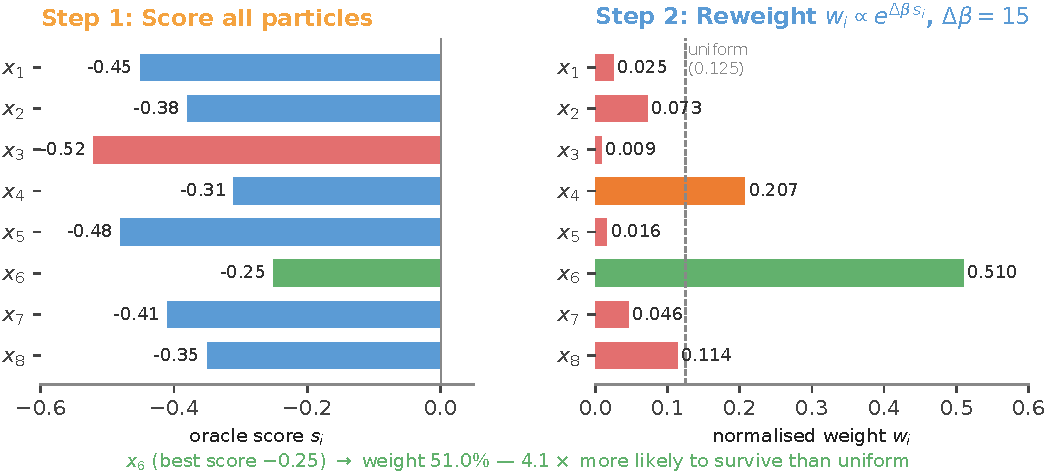
\includegraphics[width=0.95\linewidth]{figures/fig_gpa_walkthrough_score.pdf}
\caption{Score and reweight on the $N\!=\!8$ toy. \textbf{Left:} per-particle oracle scores $s_i$ (best in green: $x_6\!=\!-0.25$; worst in red: $x_3\!=\!-0.52$). \textbf{Right:} normalised weights after the tilt $w_i\!\propto\!\exp(\Delta\beta\,s_i)$ at $\Delta\beta\!=\!15$; uniform $1/N\!=\!0.125$ shown dashed. $x_6$ collects $51.0\%$ of the mass---$4.1\!\times$ the uniform expectation.}
\label{fig:walkthrough-score}
\end{figure}

\subsection{Adapting $\Delta\beta$ via bisection on $\ESS$}

The ESS-adaptive schedule (Lemma~\ref{lem:ess}) chooses $\Delta\beta_t$ so that $\ESS\!\geq\!\alpha N$ \emph{exactly} (not below). With $\alpha\!=\!0.5$, the target is $\ESS_{\rm target}\!=\!4$. Algorithm~\ref{alg:bisect} runs 64 bisection iterations on $[\Delta\beta_{\min}, \Delta\beta_{\max}]\!=\![0,1000]$.

\begin{algorithm}[h]
\caption{Bisection for $\Delta\beta$ given $\ESS$ target}\label{alg:bisect}
\begin{algorithmic}[1]
\State \textbf{Input:} scores $\{r_i\}_{i=1}^N$, target $\tau N$, range $[\Delta\beta_{\min}, \Delta\beta_{\max}]$, max iters $T_{\rm bs}$
\For{$t\!=\!1,\dots,T_{\rm bs}$}
    \State $\Delta\beta_{\rm mid}\!\leftarrow\!(\Delta\beta_{\min}+\Delta\beta_{\max})/2$
    \State $w_i\!\leftarrow\!\exp(\Delta\beta_{\rm mid}\,r_i)/Z$, with $Z\!=\!\sum_j\exp(\Delta\beta_{\rm mid}\,r_j)$
    \State $\ESS\!\leftarrow\!1/\sum_i w_i^2$
    \If{$\ESS > \tau N$} $\Delta\beta_{\min}\!\leftarrow\!\Delta\beta_{\rm mid}$ \Comment{can push harder}
    \Else \;$\Delta\beta_{\max}\!\leftarrow\!\Delta\beta_{\rm mid}$ \Comment{too aggressive}
    \EndIf
\EndFor
\State \textbf{Return:} $\Delta\beta_{\min}$
\end{algorithmic}
\end{algorithm}

For our example, the bisection converges to $\Delta\beta\!\approx\!11.7$, giving $\ESS\!\approx\!4.0\!=\!\alpha N$. The hand-picked $\Delta\beta\!=\!15$ above (which produced $\ESS\!=\!3.08$) was therefore more aggressive than the auto-schedule would choose.

\begin{figure}[h]
\centering
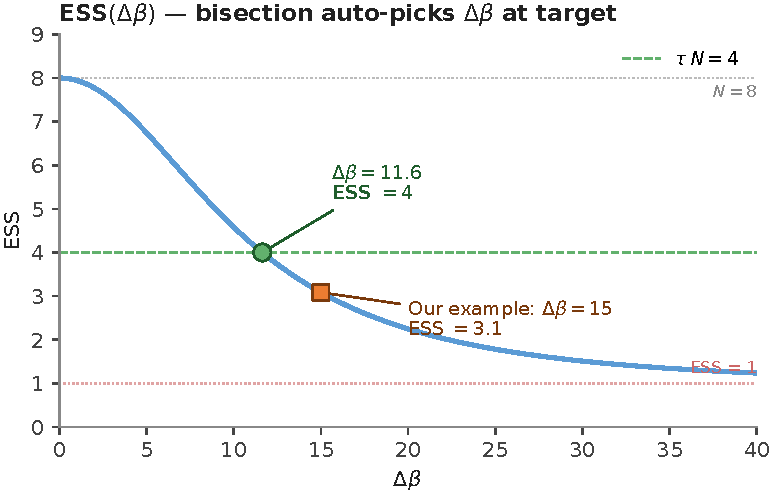
\includegraphics[width=0.78\linewidth]{figures/fig_gpa_walkthrough_ess.pdf}
\caption{$\ESS(\Delta\beta)$ for the $N\!=\!8$ toy oracle scores. The function decreases monotonically from $\ESS\!=\!N$ at $\Delta\beta\!=\!0$ toward $\ESS\!=\!1$ as $\Delta\beta\!\to\!\infty$ (winner-take-all). Bisection finds the unique $\Delta\beta\!=\!11.7$ at which $\ESS$ hits the target $\tau N\!=\!4$ (green dot). The hand-picked $\Delta\beta\!=\!15$ used in the walk-through (orange square) is past the target and so over-collapses the population.}
\label{fig:walkthrough-ess}
\end{figure}

\subsection{Resampling: multinomial vs.\ systematic}

\paragraph{Multinomial.} Draw counts $\!=\!(c_1,\dots,c_N)\!\sim\!\mathrm{Multinomial}(N, w)$. Expected copies per particle are $\E[c_i]\!=\!N\!\cdot\!w_i$, but the realised counts are noisy.

\paragraph{Systematic.} Lay the weights end-to-end as a unit interval $[0,1]$ (segment $i$ has width $w_i$). Drop $N$ pointers at positions $u\!+\!k/N$ for $k\!=\!0,\dots,N\!-\!1$, with $u\!\sim\!\mathrm{Uniform}[0,1/N)$. Particle $i$ receives a number of copies equal to the count of pointers in its segment. This has identical mean to multinomial but lower variance, and is the default in \gpa{}.

For our $N\!=\!8$ example with $u\!=\!0$, the eight pointers at $\{0.000, 0.125, 0.250, 0.375, 0.500, 0.625, 0.750, 0.875\}$ land in segments as follows: $w_2$ (cumulative 0.025--0.098) captures pointer 0.097; $w_4$ (0.107--0.314) captures pointers at 0.125, 0.250; $w_6$ (0.330--0.840) captures pointers at 0.375, 0.500, 0.625, 0.750; $w_8$ (0.886--1.000) captures pointer 0.875. Final copy counts:
\begin{center}
\begin{tabular}{lcccccccc}
\toprule
$i$       & 1 & 2 & 3 & 4 & 5 & 6 & 7 & 8 \\
copies    & 0 & 1 & 0 & 2 & 0 & 4 & 0 & 1 \\
\bottomrule
\end{tabular}
\end{center}
Four particles ($x^1, x^3, x^5, x^7$) are eliminated; $x^6$ is duplicated four times. After resampling, weights reset to $1/N\!=\!0.125$ uniformly.

\begin{figure}[h]
\centering
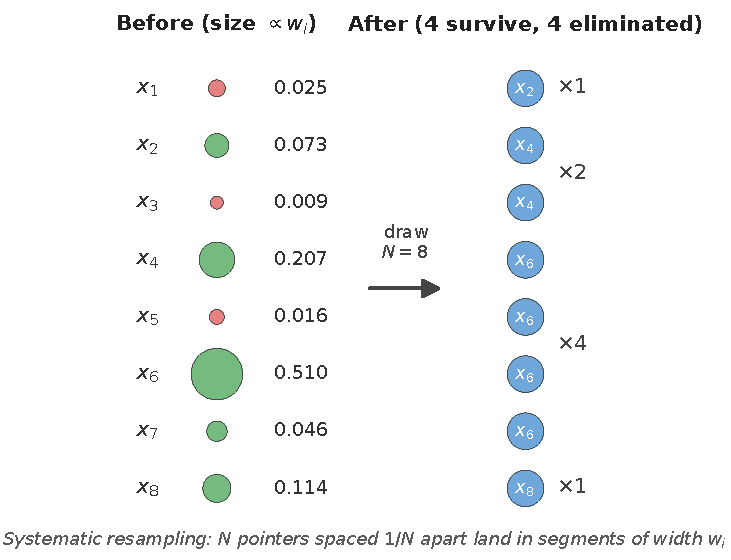
\includegraphics[width=0.85\linewidth]{figures/fig_gpa_walkthrough_resample.pdf}
\caption{Systematic resampling of the $N\!=\!8$ toy. \textbf{Left:} bubble area is proportional to $w_i$; green = retained, red = eliminated by the resampling step. \textbf{Right:} after resampling, all weights reset to $1/N$; $x_6$ now appears four times, $x_4$ twice, $x_2$ and $x_8$ once each. Four particles ($x_1, x_3, x_5, x_7$) are eliminated.}
\label{fig:walkthrough-resample}
\end{figure}

\subsection{Mutation: partial mask + denoise on a length-12 DNA toy}

Each of the eight resampled (now duplicate-rich) particles is independently mutated by $K_\beta$. Concretely, with mask fraction $\mathrm{nf}\!=\!0.25$ ($\!\to\!\lceil 0.25\!\cdot\!12\rceil\!=\!3$ positions on a length-12 sequence):
\begin{center}
\begin{tabular}{ll}
\toprule
\textbf{Step}        & \textbf{Sequence} \\
\midrule
Before (a duplicate of $x^6$)   & \texttt{ACGTATGCACGT} \\
Random mask 3 positions          & \texttt{AC?TA?GC?CGT} \\
Denoise via $p_\theta$           & \texttt{AC\textbf{T}TA\textbf{A}GC\textbf{A}CGT} \\
\midrule
Net edits                         & pos 3: G$\to$T; \, pos 6: T$\to$A; \, pos 9: C$\to$A \\
\bottomrule
\end{tabular}
\end{center}
Two properties this kernel inherits from the pretrained $p_\theta$:
\begin{itemize}
\item \emph{Grammar preservation.} The denoiser sees the unmasked context and proposes tokens consistent with whatever motif/composition rules $p_\theta$ has learned. Random per-position resampling would not.
\item \emph{Diversity restoration.} The four duplicates of $x^6$ each get an \emph{independent} random mask + denoising pass, so they diverge into four distinct child sequences. Without mutation the population would collapse to four identical copies.
\end{itemize}
The mask fraction $\mathrm{nf}$ controls exploration: $\mathrm{nf}\!=\!0.05$ is local search ($\sim\!10$ positions per step on a 200-bp DNA enhancer), $\mathrm{nf}\!=\!0.20$ is large jumps. Section~\ref{sec:results:ablation} reports sensitivity in the practical range.

%-----------------------------------------------------------------------
\section{Hyperparameters}\label{app:hyper}

Table~\ref{tab:hyper-rerd} lists hyperparameters for the SMC-protocol comparison (\drakes{} eval pair); Table~\ref{tab:hyper-ctrldna} lists those for \ctrldna{} comparison (HyenaDNA + gReLU MSE oracles); Table~\ref{tab:hyper-dnacraft} for \dnacraft{} comparison (HyenaDNA/DiMamba + Enformer 50/50). Default values are bolded.

\begin{table}[h]
\caption{Hyperparameters for the SMC-protocol comparison (HepG2 enhancer, MDLM backbone, \drakes{} split-oracle).}
\label{tab:hyper-rerd}
\centering
\small
\begin{tabular}{lll}
\toprule
Parameter & Mean recipe & Spec recipe \\
\midrule
$N$ (population) & 5000 & 5000 \\
$\alpha$ (ESS threshold) & 0.5 & 0.5 \\
$\beta_*$ (target inverse temp) & 200 & 100 \\
$T_{\max}$ (max steps) & 30, hard cap 200 & 30, hard cap 200 \\
nf (mask fraction) & 0.05 & 0.05 \\
DPS gradient strength $\eta$ & 3000 & 3000 \\
$\mathrm{pw}$ (off-target penalty) & 0 & 0.35 \\
GC bio-filter & [0.45, 0.55] & [0.45, 0.55] \\
\bottomrule
\end{tabular}
\end{table}

\begin{table}[h]
\caption{Hyperparameters for \ctrldna{} comparison (Reddy promoters, HyenaDNA backbone, gReLU MSE oracles, universal recipe).}
\label{tab:hyper-ctrldna}
\centering
\small
\begin{tabular}{ll}
\toprule
Parameter & Universal recipe \\
\midrule
$N$ (population) & 10000 \\
$\alpha$ (ESS threshold) & 0.5 \\
$\beta_*$ & 100 \\
$T_{\max}$ (steps) & 60 \\
nf (mask fraction) & 0.05 \\
$K$ (branch factor) & 8 \\
$\mathrm{pw}$ & 0.35 \\
diversity $\lambda$ (conformity) & \textbf{1.0} \\
DPS & off \\
GC bio-filter & off \\
\bottomrule
\end{tabular}
\end{table}

\begin{table}[h]
\caption{Hyperparameters for \dnacraft{} comparison (Gosai 50/50 split, top-128 by MinGap-Eval). C1 = no GC penalty; C3 = soft GC penalty (gct=0.60), no hard bio-filter.}
\label{tab:hyper-dnacraft}
\centering
\small
\begin{tabular}{lll}
\toprule
Parameter & C1 & C3 \\
\midrule
$N$ (population) & 5000 & 5000 \\
$\beta_*$ & 25 & 25 \\
$\mathrm{pw}$ & 0.30 & 0.30 \\
DPS & on & on \\
GC penalty (gct) & --- & 0.60 \\
GC bio-filter & off & off \\
$K$ & 8 & 8 \\
\bottomrule
\end{tabular}
\end{table}

%-----------------------------------------------------------------------
\section{Full GPA-vs-ISM/LEDIDI tables}\label{app:ism_full}

Single-sequence comparison: GPA row = the one sequence in each pool that maximises $\mathrm{AG}-\mathrm{LN}$ (sweet spot: low LN, high held-out AG). Directly comparable to \ism{}/\ledidi{} which are inherently single-sequence.

\begin{table}[h]
\caption{Single-sequence comparison, K562 enhancer, two seeds (uid=181692 natural, uid=50178 random). \gpa{} row = argmax of $\mathrm{AG}-\mathrm{LN}$ within the 5{,}000-seq pool.}
\label{tab:ism_singleseq}
\centering
\small
\begin{tabular}{llrrr}
\toprule
Seed & Method & Edits & LN & AG \\
\midrule
\multirow{4}{*}{uid=181692}
 & \gpa{} (no DPS) uncap   &  96 & 4.97 & \textbf{3.33} \\
 & \gpa{} (+DPS) cap30     &  60 & 6.21 & \textbf{3.47} \\
 & \ism{} gen 115          & 115 & 8.74 & 2.83 \\
 & \ledidi{} t15 $\lambda$=0.05 & 125 & 9.81 & $-$0.22 \\
\midrule
\multirow{4}{*}{uid=50178}
 & \gpa{} (no DPS) cap30   &  60 & 4.71 & 2.75 \\
 & \gpa{} (+DPS) cap30     &  59 & 6.58 & \textbf{3.61} \\
 & \ism{} gen 115          & 115 & 9.58 & 2.92 \\
 & \ledidi{} t15 $\lambda$=0.05 & 105 &11.66 & $-$0.62 \\
\bottomrule
\end{tabular}
\end{table}

\paragraph{Reading the table.}
A single \gpa{} sequence (e.g.\ +DPS cap30 on uid=50178: LN $6.58$, AG $3.61$) beats \ism{} gen 115 on the held-out AG by $+0.69$ at LN $\sim\!3.0$ lower—better held-out activity \emph{and} less reward-hacking. Under any selection rule, \ledidi{} stays AG-negative; not one of its 50 reruns produces an AG-positive sequence.

\paragraph{Apples-to-apples runtime (single H100, K562 enhancer, 5{,}000-sequence pool).}
Table~\ref{tab:ism_runtime} reports wall-time at matched output volume, averaged across the random and natural pools. \gpa{} is fully population-parallel: a single SMC step propagates all 5{,}000 particles together through the diffusion proposal, so the per-particle cost is the GPU-memory chunk \texttt{mutation\_batch\_size=128} amortised over the population. \ism{} is also nominally population-parallel (5{,}000 independent greedy trajectories), but its sequential cost is fixed at 115 generations per seed, and that dominates wall regardless of how memory chunks are batched. \ledidi{} is chunked-sequential by design: 5{,}000 seeds processed in 39 chunks of 128 along the Gumbel-softmax optimisation. The result is $\sim\!9.3\times$ speedup over \ism{} and $\sim\!3.4\times$ speedup over \ledidi{} at identical pool size and identical hardware.

\begin{table}[h]
\caption{Apples-to-apples runtime: single H100, 5{,}000-sequence K562-enhancer pool, averaged across random and natural seed pools. \gpa{} = v3 noDPS recipe (matches Sec.~\ref{sec:results:ism}). Speedup column is $\mathrm{wall}_{\text{baseline}}/\mathrm{wall}_{\gpa{}}$.}
\label{tab:ism_runtime}
\centering
\small
\begin{tabular}{lllr}
\toprule
Method & Wall (5K pool) & Parallelism & Speedup vs.\ \gpa{} \\
\midrule
\textbf{\gpa{}} & \textbf{$\sim\!11.6$ min} & population-parallel (5{,}000 SMC particles) & --- \\
\ledidi{}       & $\sim\!40$ min     & chunked-sequential (39 chunks $\times$ 128 seeds) & $\sim\!3.4\times$ slower \\
\ism{}          & $\sim\!107.5$ min  & population-parallel, but 115 sequential greedy gens & $\sim\!9.3\times$ slower \\
\bottomrule
\end{tabular}
\end{table}

%-----------------------------------------------------------------------
\section{Full DNA-CRAFT tables (GPA-C1 vs GPA-C3)}\label{app:dnacraft_full}

The headline column in Table~\ref{tab:dnacraft} uses GPA-C3 (\texttt{dps\_pw030\_b25\_gct060\_nobio}). This appendix shows the same benchmark with the alternate recipe variant GPA-C1 (\texttt{dps\_pw030\_b25}, no GC penalty), under the matched-output-budget protocol of Table~\ref{tab:dnacraft} (\texttt{by\_pool\_composite} top-64 from \texttt{gpa\_output\_best\_eval.h5}, 3 reps for both variants). Both variants run at $\sim\!3.6$ min/seed (no MCTS) on the MDLM backbone; the only difference is the soft GC-centering term added to C3's DPS gradient.

\paragraph{Recipe decomposition.}
Each token in the recipe name maps to a specific knob in the GPA algorithm of \S\ref{sec:method}, with no other differences between the two variants:
\begin{itemize}
\item \texttt{dps} -- enables the Gumbel-softmax oracle gradient with strength $\eta\!=\!3000$ (\S\ref{sec:method:ext}, ``Gumbel-softmax oracle gradient (DPS)''). This is a biased proposal in the sense of \S\ref{sec:method:ext} and is shared by both C1 and C3, so the C1$\leftrightarrow$C3 contrast does not move along the DPS-bias axis.
\item \texttt{pw030} -- sets the off-target weight $\mathrm{pw}\!=\!0.30$ in the linear fitness of Eq.~\ref{eq:fitness} (\S\ref{sec:method:pw}); the same $0.30$ weights the off-target term inside the DPS gradient as well.
\item \texttt{b25} -- sets the SMC tilt ceiling $\beta_*\!=\!25$. This is below the default range $\beta_*\!\in\!\{100,200\}$ in \S\ref{sec:exp} and is a deliberately gentler tilt that preserves population diversity at some cost in MinGap; both variants share it.
\item \texttt{gct060} \emph{(C3 only)} -- adds a quadratic centering term $-w\,(g(x)-0.60)^2$ to the DPS objective before backpropagation, where $g(x)\!=\!\overline{P(C)+P(G)}$ is the per-position soft-onehot GC fraction and $w\!=\!10$. The penalty rides inside the same Gumbel-softmax gradient that DPS already computes; it is \emph{not} a hard accept/reject filter.
\item \texttt{nobio} -- disables the hard bio-filter (no \texttt{gc\_low}/\texttt{gc\_high} interval gating). All GC discipline in C3 therefore comes from the soft \texttt{gct060} term in the DPS gradient.
\end{itemize}
Both variants additionally use the default branch factor $K\!=\!8$ (\S\ref{sec:method:ext}, Prop.~\ref{prop:K}) and population $N\!=\!5{,}000$ (Table~\ref{tab:dnacraft} caption), so both target $\pi_{\beta_*}^{(K=8)}\!\neq\!\pi_{\beta_*}$ in the sense of Prop.~\ref{prop:K}; the C1$\leftrightarrow$C3 contrast isolates the GC-centering term with $K$, $\beta_*$, $\mathrm{pw}$, $N$, and the DPS bias all held constant.

\begin{table}[h]
\caption{\dnacraft{} benchmark with the GPA-C1 alternate recipe (\texttt{dps\_pw030\_b25}; no GC penalty), reported alongside the headline GPA-C3 (Table~\ref{tab:dnacraft}). Both columns: \texttt{by\_pool\_composite} top-64 from \texttt{gpa\_output\_best\_eval.h5}, mean (std) over 3 reps. Baselines verbatim from \citet{dnacraft2026}.}
\label{tab:dnacraft_full_eval}
\centering
\scriptsize
\begin{tabular}{llcccccccccc}
\toprule
Cell & Metric & SMC & CG & TDS & DRAKES & D3 & Ledidi & Ctrl-DNA & DNA-CRAFT & \gpa{}-C1 & \gpa{}-C3 \\
\midrule
\multirow{4}{*}{HepG2}
 & MinGap   & 1.61 & $-$0.23 & 0.40 & $-$1.40 & 0.05 & 5.77 & \textbf{7.79} & 4.35 & 6.87 & 6.91 \\
 & Motif    & 0.55 & 0.86 & 0.40 & 0.06 & 0.87 & 0.58 & 0.63 & \textbf{0.92} & 0.90 & \textbf{0.92} \\
 & 3-mer    & 0.81 & 0.97 & 0.74 & $-$0.36 & \textbf{0.98} & 0.76 & 0.49 & \textbf{0.98} & 0.95 & 0.95 \\
 & Diversity& 0.83 & \textbf{1.98} & 0.96 & 1.86 & \textbf{1.98} & \textbf{1.98} & 1.90 & \textbf{1.98} & 1.81 & 1.86 \\
\midrule
\multirow{4}{*}{K562}
 & MinGap   & 4.12 & 0.00 & 1.62 & $-$0.20 & 0.18 & 7.66 & \textbf{9.07} & 5.69 & 8.18 & 8.13 \\
 & Motif    & 0.45 & 0.85 & 0.51 & 0.14 & 0.86 & 0.65 & 0.63 & 0.93 & 0.93 & \textbf{0.94} \\
 & 3-mer    & 0.66 & 0.94 & 0.65 & $-$0.35 & 0.96 & 0.69 & 0.41 & \textbf{0.98} & 0.92 & 0.95 \\
 & Diversity& 0.31 & \textbf{1.98} & 0.64 & 1.96 & \textbf{1.98} & \textbf{1.98} & 1.90 & \textbf{1.98} & 1.56 & 1.83 \\
\midrule
\multirow{4}{*}{SK-N-SH}
 & MinGap   & 0.56 & $-$0.28 & 0.19 & 0.09 & $-$0.01 & 3.03 & 3.72 & 3.23 & \textbf{5.07} & 4.98 \\
 & Motif    & 0.52 & 0.86 & 0.48 & 0.23 & 0.84 & 0.38 & 0.48 & 0.88 & 0.89 & \textbf{0.92} \\
 & 3-mer    & 0.78 & 0.95 & 0.72 & $-$0.38 & 0.93 & 0.37 & 0.20 & \textbf{0.97} & 0.87 & 0.94 \\
 & Diversity& 1.27 & \textbf{1.98} & 0.92 & 1.83 & 1.97 & \textbf{1.98} & 1.86 & \textbf{1.98} & 1.59 & 1.86 \\
\bottomrule
\end{tabular}
\end{table}

\paragraph{Reading.}
GPA-C1 and GPA-C3 give nearly tied MinGap and Motif Spearman on every cell (within seed std on most rows). C3 wins Motif on HepG2 / K562 / SK-N-SH ($+0.02$/$+0.01$/$+0.03$) and 3-mer on K562 / SK-N-SH ($+0.03$/$+0.07$). The biggest practical difference is Diversity: the soft GC-centering term in C3's DPS gradient recovers $+0.05$ to $+0.27$ Shannon bits over C1 on every cell, lifting C3 above the Ctrl-DNA Diversity floor on all three cells. The mechanism is indirect: by penalising drift away from $g(x)\!=\!0.60$ at every Gumbel-softmax step, the term blunts the oracle's tendency to push particles toward narrow high-GC modes, which in turn keeps the population spread out in sequence space. C1 wins MinGap on K562 / SK-N-SH ($+0.05$/$+0.09$) but loses across the rest. C3 is the headline because the +Diversity / +Motif / +3-mer trade dominates the small MinGap give-back; C1 is reported as an ablation that isolates the GC-penalty's contribution.

\paragraph{Backbone caveat.}
\dnacraft{}'s reported numbers in Table~\ref{tab:dnacraft} are obtained on a Mamba-style discrete-diffusion (DiMamba) backbone whose code and pretrained checkpoints are not publicly available; the same paper also reports DiMamba-vs-MDLM ablations that show DiMamba contributes additional biological-faithfulness gains. Our \gpa{}-C1 / \gpa{}-C3 numbers are obtained on the publicly available MDLM backbone of \citet{sahoo2024mdlm} and should be read as a lower bound on what \gpa{} would achieve at backbone parity, by Remark~\ref{rem:agnostic}.

%-----------------------------------------------------------------------
\section{Wall-time table}\label{app:wall}

\begin{table}[h]
\caption{Wall time per seed and 5-seed totals (HepG2, identical H100 hardware, identical HyenaDNA backbone). Wall time excludes downstream motif scoring.}
\label{tab:wall}
\centering
\small
\begin{tabular}{lrr}
\toprule
Method & Wall/seed (h) & 5-seed total (GPU-h) \\
\midrule
\ctrldna{} R200 (RL fine-tune) & $43.5\pm 0.8$ & $\sim\!218$ \\
\gpa{} v3 (K=8, no diversity)  & $3.97\pm 0.59$ & 19.8 \\
\gpa{} v4 (K=8 + rejuvenation) & $2.17\pm 0.22$ & 10.8 \\
\gpa{} v5 (K=8 + diversity)    & $\mathbf{2.22\pm 0.52}$ & $\mathbf{11.1}$ \\
\bottomrule
\end{tabular}
\end{table}

%-----------------------------------------------------------------------
\section{DPS gradient ablation}\label{app:dps_ablation}

Population annealing alone (no DPS) already beats single-chain refinement baselines; DPS gradient is a multiplicative enhancement.

\begin{table}[h]
\caption{DPS gradient ablation on Gosai HepG2.}
\label{tab:dps_ablation}
\centering
\small
\begin{tabular}{llrrr}
\toprule
Track & Metric & \gpa{}-only & \gpa{}+DPS & $\Delta$(DPS) \\
\midrule
Mean & $H_{\mathrm{eval}}$ & $8.73\pm 0.50$ & $\mathbf{10.06\pm 0.19}$ & $+1.33$ \\
Mean & Spec & 1.58 & 3.06 & $+1.48$ \\
Spec & $H_{\mathrm{eval}}$ & $8.28\pm 0.12$ & $9.35\pm 0.20$ & $+1.07$ \\
Spec & Spec & $6.11\pm 1.45$ & $\mathbf{7.61\pm 0.25}$ & $+1.50$ \\
\bottomrule
\end{tabular}
\end{table}

%-----------------------------------------------------------------------
\section{Naturalness audit}\label{app:naturalness}

\begin{table}[h]
\caption{Naturalness audit (HepG2 top-128). \gpa{} produces bio-plausible sequences by construction; \ctrldna{} reward-hacks to non-biological space.}
\label{tab:nat}
\centering
\small
\begin{tabular}{lrrr}
\toprule
Metric & Real (Gosai) & \gpa{} & \ctrldna{} \\
\midrule
GC mean & 0.44 & 0.41 & 0.45 \\
\textbf{bio\_pass\_rate} & 0.51 & $\mathbf{1.00}$ & $\mathbf{0.05}$ \\
max homopolymer & 5.4 & 5.1 & $\mathbf{20.9}$ \\
$k$=3 Pearson & 1.0 & 0.61 & 0.39 \\
HNF1A enrichment & $0\times$ & $10\,040\times$ & $7\,812\times$ \\
\bottomrule
\end{tabular}
\end{table}

\begin{figure}[h]
\centering
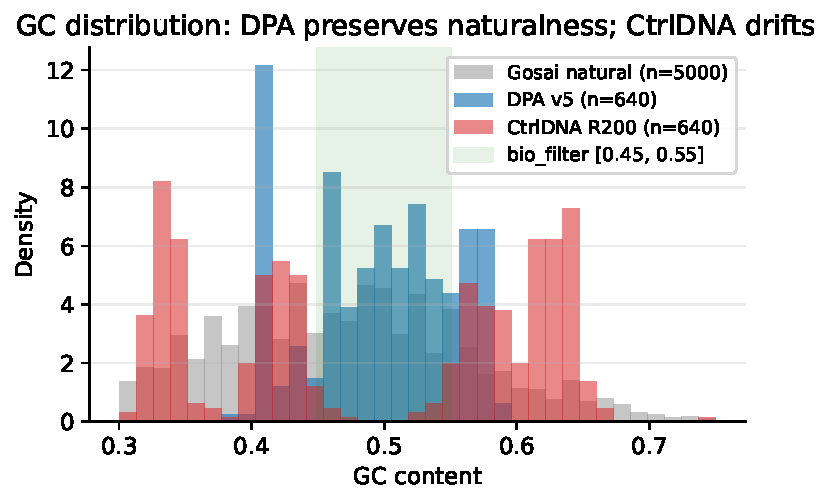
\includegraphics[width=0.6\linewidth]{figures/fig2_gc.pdf}
\caption{GC distribution comparison on HepG2 top-128 sequences. \gpa{} (blue) clusters near the lower edge of the bio-filter (45\%) but stays within the natural Gosai range (gray); \ctrldna{} (red) drifts widely, with a heavy tail of low- and high-GC sequences and a substantial fraction outside the natural distribution.}
\label{fig:gc}
\end{figure}

%-----------------------------------------------------------------------
\section{Extreme specificity}\label{app:extreme}

Pushing $\mathrm{pw}$ beyond the canonical $0.35$ trades $H_{\mathrm{eval}}$ for higher specificity until both off-targets fall below baseline (Table~\ref{tab:extreme}).

\begin{table}[h]
\caption{Extreme-specificity extension on Gosai HepG2 (single run each, $N\!=\!5000$).}
\label{tab:extreme}
\centering
\small
\begin{tabular}{rrrrr}
\toprule
$\mathrm{pw}$ & $H_{\mathrm{eval}}$ & $K_{\mathrm{eval}}$ & $S_{\mathrm{eval}}$ & $H{>}8 \wedge K{<}0 \wedge S{<}0$ \\
\midrule
0.35 & 9.65 & 2.15 &  1.10 & 0 \\
0.50 & 9.54 & 1.96 &  0.63 & 0 \\
0.70 & 8.73 & 1.52 &  0.35 & 0 \\
1.00 & 8.57 & 0.69 & $-$0.48 & 26 \\
1.50 & $\mathbf{8.44}$ & 0.55 & $\mathbf{-0.66}$ & $\mathbf{54}$ \\
\bottomrule
\end{tabular}
\end{table}

\paragraph{Beta trajectory.}
Figure~\ref{fig:beta} shows a representative ESS-adaptive $\beta$ trajectory and the population-mean reward over SMC steps for a HepG2 run.

\begin{figure}[h]
\centering
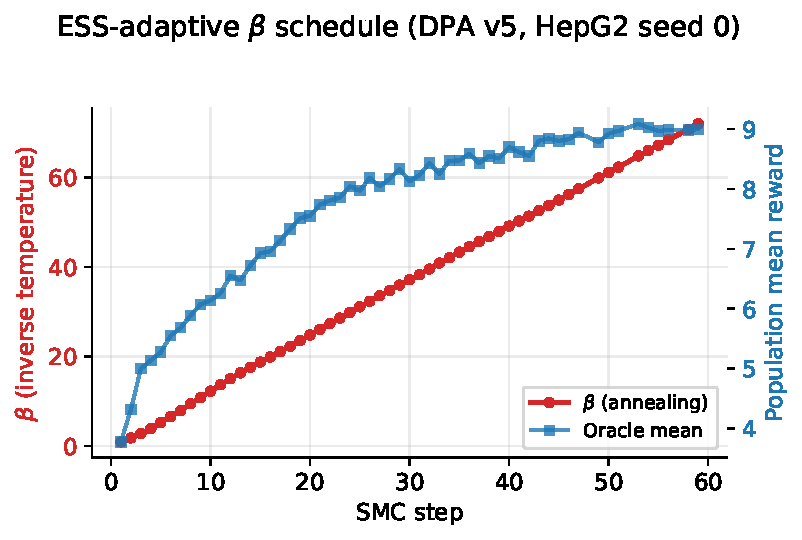
\includegraphics[width=0.6\linewidth]{figures/fig4_beta_traj.pdf}
\caption{Representative \gpa{} run trajectory (HepG2, seed 0). Red trace: ESS-adaptive $\beta$ schedule rises through the annealing path. Blue trace: population mean reward grows monotonically toward saturation as $\beta$ increases.}
\label{fig:beta}
\end{figure}

%-----------------------------------------------------------------------
\section{Negative result: APF correction for $\epsilon$-greedy $K$-branching}\label{app:apf}

A natural attempt to recover Shannon under $K$-branching is to soften the argmax with $\epsilon$-greedy ($\tau\!>\!0$ softmax over the $K$ siblings) and apply the auxiliary-particle-filter weight correction \citep{pittshephard1999}:
\[
w_{\mathrm{new}} = w_{\mathrm{old}}\big/p_\tau(\mathrm{winner}),\qquad p_\tau(j)=\exp(r_j/\tau)\big/\sum_m\exp(r_m/\tau).
\]
Compute the expectation:
\[
\E[w_{\mathrm{new}}\,\varphi(x_{\mathrm{winner}})] = \E_{x_{1:K}\sim q}\!\!\left[\sum_{j=1}^K \frac{\exp(r_j/\tau)}{\sum_m\exp(r_m/\tau)}\cdot\frac{\sum_m\exp(r_m/\tau)}{K\exp(r_j/\tau)}\,\varphi(x_j)\right]=\frac{1}{K}\sum_j \E_q[\varphi(x_j)],
\]
i.e.\ the corrected estimator is equivalent to a single-child sample. The $K$ siblings collapse and the effective-$\beta$ boost vanishes. Empirically, on a synthetic linear reward $r(x)\!=\!3x$ with $q$ uniform on $[0,1]$ (200K Monte-Carlo trials):
\begin{center}
\small
\begin{tabular}{lrrr}
\toprule
Variant & $\E[x]$ & $\mathrm{Var}[x]$ & ESS \\
\midrule
$K=1$ no selection                & 0.5000 & 0.0833 & 100.0\% \\
$K=8$ argmax (no correction)      & 0.8887 & 0.0099 & 100.0\% \\
$K=8$ softmax $\tau\!=\!0.3$ (no corr.) & 0.8445 & 0.0180 & 100.0\% \\
\textbf{$K=8$ softmax $\tau\!=\!0.3$ + APF} & 0.4880 & 0.0874 & 0.4\% \\
$K=8$ softmax $\tau\!=\!1.0$ + APF & 0.5009 & 0.0829 & 53.1\% \\
\bottomrule
\end{tabular}
\end{center}
ESS collapses at low $\tau$ and the corrected mean/variance reproduces $K=1$. We therefore do \emph{not} use APF correction for production runs and report only argmax $K$-branching. K-annealing schedules and waste-free SMC \citep{dau2022wastefree} remain valid theoretical alternatives, deferred to future work.

%-----------------------------------------------------------------------
\section{Negative result: post-hoc Metropolis tempering}\label{app:posthoc}

Another natural Shannon-rescue move is to load the concentrated argmax-$K$ pool and run Metropolis–Hastings at lower $\beta'$ to spread the population. We tested this on the K562 promoter pool (50 MH steps, nf=0.05, HyenaDNA proposal):

\begin{center}
\small
\begin{tabular}{rrrrr}
\toprule
$\beta'$ & accept rate & $\Delta$comp & $\Delta$tgt & $\Delta H$ \\
\midrule
25 &  3.4\% & $+0.02$ & $-0.06$ & $+0.05$ \\
12 &  6.5\% & $-0.15$ & $-0.27$ & $+0.10$ \\
 6 & 13.1\% & $-0.68$ & $-0.77$ & $+0.21$ \\
 3 & 29.1\% & $-2.12$ & $-2.22$ & $+0.39$ \\
 1 & 73.7\% & $-4.71$ & $-5.35$ & $+0.61$ \\
\bottomrule
\end{tabular}
\end{center}
The Pareto slope is $\sim\!3\!-\!5$ target units per $0.1$ nat of Shannon, far too steep for the diversity gap to \dnacraft{}/\ctrldna{} K562 ($\sim\!0.5$ nat) to be closed without erasing the target advantage. Increasing chain length or shrinking nf does not change the local-neighborhood geometry. The honest reading: under sharply peaked oracles, the activity–diversity tension is in the reward landscape, not the sampler.

%-----------------------------------------------------------------------
\section{GC distribution and floor-hugging}\label{app:gc}

Even with the bio-filter $\mathrm{GC}\!\in\![0.45,0.55]$, $60\!-\!75\%$ of \gpa{} top-128 sequences cluster at the lower bound. Two facts:
\begin{enumerate}
\item This is a property of the \emph{masked-diffusion proposal} at low noise fraction. At $\mathrm{nf}\!=\!0.20$ the bias inverts toward the upper bound (GC $\approx\!0.54$); the crossover occurs near $\mathrm{nf}\!\approx\!0.16\!-\!0.17$.
\item The eval oracle is GC-agnostic: at both $\mathrm{nf}$ extremes, top-128 oracle scores are comparable. The GC bias arises from $p_\theta$, not from the reward signal.
\end{enumerate}
Three mitigations were tested with mixed success: (i) GC-aware DPS gradient (\verb|gc_dps_weight|) reduces floor-hugging from $61.5\%$ to $55.0\%$ at $-0.09$ $H_{\mathrm{eval}}$ cost; (ii) narrow $1\%$ GC bands achieve uniform GC by construction at $-0.25$ $H_{\mathrm{eval}}$; (iii) stratified resampling within $2\%$ GC bins \citep{verge2015island} achieves balanced coverage at $-0.50$ to $-1.0$ $H_{\mathrm{eval}}$. We report all three options in the codebase but use the unmitigated baseline in the headline tables for fair comparison with peer methods.

%-----------------------------------------------------------------------
\section{Ctrl-DNA enhancer comparison (V7 main + V5/V8 ablations)}\label{app:ctrldna_enhancer}

This appendix gives the dedicated \ctrldna{}-vs-\gpa{} enhancer comparison referenced in \S\ref{sec:results:promoter}. Same Gosai 50/50 split as the \dnacraft{} benchmark, top-128 selection per cell, 5 \gpa{} seeds. The headline GPA recipe is V7 (universal: $K\!=\!8$, diversity $\lambda\!=\!1.0$); V8a, V8b (alternative pairwise-suppression formulations) and V5 (the previous default with $\lambda\!=\!0.2$) are ablations.

\begin{table}[h]
\caption{Ctrl-DNA vs.\ \gpa{} on Gosai HepG2/K562/SKNSH enhancers (5 seeds; mean (std)). Headline = V7 universal recipe; V8a (log\_ratio + pw=1.0), V8b (linear + pw=1.0) and V5 ($\lambda\!=\!0.2$) are ablations of the diversity / pairwise-suppression knob. \texttt{target\_raw} = mean target oracle score; \texttt{ΔR} = normalised target minus mean off-target; \texttt{shannon} = per-position entropy; \texttt{motif\_corr} = FIMO Pearson against per-cell real reference.}
\label{tab:ctrldna_enhancer}
\centering
\footnotesize
\setlength{\tabcolsep}{4pt}
\begin{tabular}{llrrrr}
\toprule
Cell & Method & target\_raw $\uparrow$ & ΔR $\uparrow$ & shannon $\uparrow$ & motif\_corr $\uparrow$ \\
\midrule
\multirow{5}{*}{HepG2}
 & \ctrldna{} R200             & 5.32 (0.65) & 0.48 (0.10) & 1.65 (0.14) & \textbf{0.29} (0.16) \\
 & \gpa{} V5 ($K\!=\!8, \lambda\!=\!0.2$) & 9.86 (0.10) & 0.85 (0.01) & 1.49 (0.03) & 0.19 (0.03) \\
 & \gpa{} V7 ($K\!=\!8, \lambda\!=\!1.0$) & \textbf{9.90} (0.12) & 0.84 (0.02) & 1.59 (0.11) & 0.20 (0.02) \\
 & \gpa{} V8a (log\_ratio, pw=1.0) & 6.61 (0.04) & 0.68 (0.01) & \textbf{1.93} (0.00) & 0.15 (0.02) \\
 & \gpa{} V8b (linear, pw=1.0) & 9.51 (0.10) & \textbf{0.93} (0.02) & 1.70 (0.11) & 0.10 (0.04) \\
\midrule
\multirow{5}{*}{K562}
 & \ctrldna{} R200             & \textbf{9.99} (1.52) & \textbf{0.77} (0.14) & 1.60 (0.15) & 0.24 (0.07) \\
 & \gpa{} V5 ($K\!=\!8, \lambda\!=\!0.2$) & 8.82 (0.13) & 0.34 (0.00) & 1.43 (0.09) & \textbf{0.26} (0.02) \\
 & \gpa{} V7 ($K\!=\!8, \lambda\!=\!1.0$) & 8.83 (0.12) & 0.32 (0.01) & 1.65 (0.02) & 0.24 (0.02) \\
 & \gpa{} V8a (log\_ratio, pw=1.0) & 6.48 (0.03) & 0.39 (0.01) & \textbf{1.94} (0.01) & 0.24 (0.01) \\
 & \gpa{} V8b (linear, pw=1.0) & 8.15 (0.04) & 0.41 (0.01) & 1.68 (0.02) & 0.25 (0.02) \\
\midrule
\multirow{5}{*}{SK-N-SH}
 & \ctrldna{} R200             & 9.93 (1.13) & \textbf{0.71} (0.10) & 1.63 (0.17) & \textbf{0.23} (0.10) \\
 & \gpa{} V5 ($K\!=\!8, \lambda\!=\!0.2$) & \textbf{14.33} (0.20) & 0.10 (0.01) & 1.49 (0.04) & \textbf{0.23} (0.01) \\
 & \gpa{} V7 ($K\!=\!8, \lambda\!=\!1.0$) & 14.17 (0.18) & 0.10 (0.00) & 1.63 (0.04) & 0.20 (0.01) \\
 & \gpa{} V8a (log\_ratio, pw=1.0) & 6.29 (0.08) & 0.22 (0.01) & \textbf{1.91} (0.01) & 0.15 (0.01) \\
 & \gpa{} V8b (linear, pw=1.0) & 8.26 (0.15) & 0.29 (0.03) & 1.74 (0.05) & 0.10 (0.01) \\
\bottomrule
\end{tabular}
\end{table}

\paragraph{Headlines.}
\gpa{} V7 (the universal recipe) wins target\_raw on HepG2 and SK-N-SH ($+4.58$ and $+4.24$ over \ctrldna{}), and is competitive on K562 within $\sim$1 std. \ctrldna{} retains a ΔR (specificity) edge on K562 and SK-N-SH at the cost of $\sim$50\% lower target activity on HepG2/SK-N-SH and high seed-to-seed variance ($\pm 1.13$--$1.52$). The V7 vs.\ V5 comparison shows the diversity-$\lambda$ bump (from $0.2$ to $1.0$) buys $+0.10$--$0.22$ shannon on every cell at zero target cost, isolating the population-conformity penalty as a strict Pareto improvement. V8a/V8b are alternative pairwise-suppression formulations: V8a (log-ratio reward, pw=1.0) achieves the tightest shannon ($1.91$--$1.94$, near uniform) but at substantial target cost; V8b (linear, pw=1.0) recovers HepG2/K562 target while maximising HepG2 ΔR. The four GPA variants together trace a Pareto front in (target, shannon, motif) space at fixed inference cost---one knob per recipe, no retraining.

%-----------------------------------------------------------------------
\section{DNA-CRAFT $K$ and $i$ scaling sweeps (UCB-MCTS variant)}\label{app:ucb_scaling}

\paragraph{Why MCTS at all.}
DNA-CRAFT replaces the SMC population with a single depth-bounded Monte Carlo Tree Search loop on a DiMamba diffusion backbone, and shows that this delivers state-of-the-art motif and 3-mer grammar fidelity on the Gosai enhancer benchmark (Table~\ref{tab:dnacraft}). The mechanism that delivers their grammar bar is plausible on its face: tree search amortises the cost of choosing the right next mutation by replaying the same scoring oracle across multiple competing children before committing—a strictly more informed proposal than picking the first child that scores well. \gpa{}'s standard $K$-branch is a depth-1 special case of this idea: try $K$ candidates from the proposal and keep the best (Sec.~\ref{sec:method:ext}). It is natural to ask whether the same \emph{deeper} planning that powers \dnacraft{}'s grammar—expanding the best leaves over multiple iterations rather than just one---closes \gpa{}'s residual gap to \dnacraft{} on motif/3-mer correlation. The \texttt{ucb\_stacked} variant exists to test exactly that question.

\paragraph{What \texttt{ucb\_stacked} does, step by step.}
At every SMC mutation step, each particle $x_t^{(j)}$ becomes the root of an independent Monte Carlo tree. We then run $i$ iterations on that tree, where each iteration follows the standard four-phase MCTS-with-UCB1 loop \citep[``UCT'';][]{kocsis2006uct}:
\begin{enumerate}
\item \emph{Selection.} Traverse from the root to a leaf by greedily picking, at each internal node $v$ with already-expanded children $\{a\}$, the child that maximises the UCB1 score \citep{auer2002ucb,kocsis2006uct}
\begin{equation}\label{eq:ucb1}
    \mathrm{UCB1}(a) \;=\; \bar{Q}(a) \;+\; c\sqrt{\frac{\ln n(v)}{n(a)}},
\end{equation}
where $\bar{Q}(a)\!\in\![0,1]$ is the mean (range-normalised) reward backed up through child $a$, $n(a)$ is the visit count of $a$, $n(v)\!=\!\sum_a n(a)$ is the parent visit count, and $c\!=\!\sqrt{2}$ is the standard exploration constant. The first term exploits children with high empirical value; the second term explores low-visit children with a $\sqrt{\log n / n(a)}$ confidence radius. Together this is the canonical bandit rule of \citet{auer2002ucb} for stochastic multi-armed bandits, and \citet{kocsis2006uct} show that applying it node-wise inside a tree (UCT) inherits the same $\mathcal{O}(\log n)$ regret bound at each node. Children with $n(a)\!=\!0$ are tried first by convention so the second term remains well-defined.
\item \emph{Expansion.} Apply \gpa{}'s standard $K$-branch operator at the selected leaf: draw $K\!=\!8$ children using partial-mask$\circ$denoise + DPS (the same operator the no-MCTS \gpa{} would use as its mutation kernel).
\item \emph{Evaluation.} Score each new child under the eval-side reward.
\item \emph{Backpropagation.} Update visit counts $n(\cdot)$ and value estimates $\bar{Q}(\cdot)$ along the path from each new child up to the root, so the next iteration's UCB1 selection (Eq.~\ref{eq:ucb1}) uses fresh statistics.
\end{enumerate}
We bound the tree depth at $d\!=\!2$, so the planner looks at most two mutation steps ahead. After $i$ iterations the tree has at most $1\!+\!i\!\cdot\!K$ nodes; the mutated state for $x_t^{(j)}$ is the highest-reward leaf in that tree. The SMC step then proceeds as usual: the new particle states are importance-weighted at the next $\beta$, resampled if $\ESS$ degenerates, and the loop continues.

\paragraph{Connection to \dnacraft{}.}
The four-step loop (UCB selection $\to$ $K$-fold expansion $\to$ scoring $\to$ reward backprop) is identical in shape to \dnacraft{}'s tree search. What differs is the \emph{scope} of where the tree sits and how it is consumed:
\begin{itemize}
\item \dnacraft{} runs \emph{one} MCTS for the whole design problem: $N_{\mathrm{iter}}\!=\!64$ iterations, $M\!=\!128$ children per expansion, full leaf-to-clean rollouts. Their MinGap-Set archive accumulates the best $N_{\max}\!=\!64$ leaves seen during the run, and that archive is the output (no SMC, no population).
\item \texttt{ucb\_stacked} runs \emph{many} MCTSs: one per particle, per SMC step. Each tree is run for $i\!\in\!\{12,18,24,36\}$ iterations with $K\!=\!8$ children per expansion at depth $d\!=\!2$, no full rollouts (we score after one denoising step). The output is the SMC population at the final $\beta$, exactly as in standard \gpa{}; the trees are only the per-particle mutation kernel.
\end{itemize}
``Stacked'' refers to the layering: MCTS sits \emph{on top of} the $K$-branch+DPS proposal in the SMC inner loop. The $K$-branch supplies the unit of expansion; UCB1+depth-2 lookahead is the planner that decides which leaf is worth expanding next. In effect, \texttt{ucb\_stacked} is a way to ask: does \dnacraft{}'s planning shape, used as a mutation kernel inside SMC, give us the same grammar advantages \dnacraft{} reports as the entire search?

\paragraph{Cost.}
Each \texttt{ucb\_stacked} mutation step performs $1\!+\!i\!\cdot\!K$ scoring calls per particle (vs.\ standard \gpa{}'s 8). At our default $K\!=\!8, i\!=\!18$ this is $145$ scoring calls per particle per step---roughly $18\!\times$ the standard \gpa{} mutation budget. The wallclock overhead is sub-linear in both axes (we report the empirical scaling laws below); for the $i\!=\!18$ headline configuration this works out to $\sim\!7\!\times$ the standard \gpa{}-C3 wallclock per seed.

\paragraph{What the tables below show.}
The two sweeps below sit on K562 and fix one axis at the pilot value while sweeping the other ($K\!=\!8$ for the $i$-sweep, $i\!=\!12$ for the $K$-sweep), at depth $d\!=\!2$ throughout. Wallclock is per seed on a single H100; all metrics are reported under the matched-output-budget protocol of Table~\ref{tab:dnacraft} (\texttt{by\_pool\_composite} top-64 from \texttt{gpa\_output\_best\_eval.h5}). Both sweeps include the standard $K\!=\!8, i\!=\!12$ pilot anchor (5 seeds) for cross-reference.

\begin{table}[h]
\caption{DNA-CRAFT $i$-axis sweep (K562, $K\!=\!8$, $d\!=\!2$). \texttt{by\_pool\_composite} top-64. 5 seeds for $i\!\in\!\{12,18\}$, 2 seeds for $i\!\in\!\{24,36\}$.}
\label{tab:ucb_i_sweep}
\centering
\small
\begin{tabular}{rrrrrrr}
\toprule
$i$ & $n$ & wall (min) & MinGap & Motif & 3-mer & Diversity \\
\midrule
12 & 5 & 31.35 (3.62) & $+$8.066 (0.063) & 0.940 (0.004) & 0.945 (0.023) & 1.903 (0.022) \\
18 & 5 & 32.26 (0.62) & $+$8.115 (0.013) & 0.942 (0.003) & 0.961 (0.003) & 1.926 (0.027) \\
24 & 2 & 37.07 (4.08) & $+$8.153 (0.075) & 0.940 (0.002) & 0.968 (0.003) & 1.941 (0.012) \\
36 & 2 & 46.60 (3.23) & $+$8.015 (0.001) & 0.941 (0.003) & 0.965 (0.002) & 1.937 (0.014) \\
\bottomrule
\end{tabular}
\end{table}

\begin{table}[h]
\caption{DNA-CRAFT $K$-axis sweep (K562, $i\!=\!12$, $d\!=\!2$). \texttt{by\_pool\_composite} top-64. 5 seeds for $K\!=\!8$ (pilot anchor), 2 seeds for $K\!\in\!\{16,24,32\}$.}
\label{tab:ucb_K_sweep}
\centering
\small
\begin{tabular}{rrrrrrr}
\toprule
$K$ & $n$ & wall (min) & MinGap & Motif & 3-mer & Diversity \\
\midrule
 8 & 5 & 31.35 (3.62) & $+$8.066 (0.063) & 0.940 (0.004) & 0.945 (0.023) & 1.903 (0.022) \\
16 & 2 & 49.39 (6.64) & $+$8.124 (0.108) & 0.939 (0.002) & 0.959 (0.008) & 1.898 (0.043) \\
24 & 2 & 69.00 (13.13) & $+$8.070 (0.016) & 0.942 (0.004) & 0.953 (0.007) & 1.935 (0.008) \\
32 & 2 & 77.40 (4.31) & $+$8.022 (0.103) & 0.936 (0.000) & 0.953 (0.002) & 1.907 (0.045) \\
\bottomrule
\end{tabular}
\end{table}

\paragraph{Reading.}
Wallclock is sub-linear in both axes ($\mathrm{wall}\propto i^{0.369}$, $R^2\!=\!0.91$; $\mathrm{wall}\propto K^{0.672}$, $R^2\!=\!0.99$): MCTS-rollout batching and K-branch parallelisation amortise cost. Under the matched-output-budget pool-composite selection, MinGap is saturated across the full $i$ and $K$ sweeps (range $8.02$--$8.15$, within seed std on every row); Motif and Diversity are also flat ($\Delta < 0.01$ across $i$, $\Delta < 0.04$ across $K$); only 3-mer Pearson shows a mild gain with $i$ ($+0.020$ from $i\!=\!12$ to $i\!=\!24$). UCB-MCTS planning therefore buys negligible additional metric gain over the standard \gpa{}-C3 headline at substantial wallclock overhead, which is why C3 (no MCTS) is the headline column in Table~\ref{tab:dnacraft} and \texttt{ucb\_stacked} is reported here only as an optional variant.

%-----------------------------------------------------------------------
\section{Population-size ($N$) ablation}\label{app:n_sweep}

The headline GPA-C3 numbers in Table~\ref{tab:dnacraft} use the standard $N\!=\!5{,}000$ SMC particle population. SMC theory predicts that the empirical distribution converges to the reward-tilted target at the parametric rate $\mathcal{O}(1/\sqrt{N})$ (Theorem~\ref{thm:smc-app}); the population-as-budget reading in \S\ref{sec:method:smc-recap} predicts \emph{monotonic improvement of every reported metric with growing $N$}. We test this directly: holding the C3 recipe and the matched-output-budget selection rule (\texttt{by\_pool\_composite} top-64) fixed, sweep $N\!\in\!\{128, 500, 1000, 2500, 5000, 10000, 20000\}$ across all three cells of the \dnacraft{} enhancer benchmark, 5 SMC seeds per $(N, \text{cell})$ pair.

\begin{table}[h]
\caption{$N$-axis ablation on the \dnacraft{} enhancer benchmark; GPA-C3 (no MCTS), \texttt{by\_pool\_composite} top-64 from \texttt{gpa\_output\_best\_eval.h5}. Mean (std) over 5 SMC seeds. Every metric improves monotonically with $N$ on every cell, validating the population-as-budget framing of \S\ref{sec:method:smc-recap}.}
\label{tab:n_sweep}
\centering
\small
\begin{tabular}{rrrrr}
\toprule
$N$ & MinGap $\uparrow$ & Motif $\uparrow$ & 3-mer $\uparrow$ & Diversity $\uparrow$ \\
\midrule
\multicolumn{5}{l}{\emph{HepG2}} \\
   128 & 6.052 (0.087) & 0.829 (0.036) & 0.757 (0.084) & 1.415 (0.101) \\
   500 & 6.559 (0.153) & 0.884 (0.022) & 0.843 (0.070) & 1.600 (0.167) \\
 1{,}000 & 6.677 (0.130) & 0.895 (0.008) & 0.923 (0.021) & 1.725 (0.104) \\
 2{,}500 & 6.788 (0.129) & 0.912 (0.005) & 0.938 (0.024) & 1.845 (0.029) \\
 5{,}000 & 6.962 (0.076) & 0.915 (0.006) & 0.952 (0.013) & 1.870 (0.056) \\
10{,}000 & 7.013 (0.189) & 0.920 (0.003) & 0.968 (0.005) & 1.908 (0.014) \\
20{,}000 & \textbf{7.081} (0.149) & \textbf{0.928} (0.006) & \textbf{0.972} (0.004) & \textbf{1.912} (0.020) \\
\midrule
\multicolumn{5}{l}{\emph{K562}} \\
   128 & 7.236 (0.160) & 0.871 (0.012) & 0.774 (0.104) & 1.515 (0.120) \\
   500 & 7.709 (0.175) & 0.915 (0.011) & 0.863 (0.044) & 1.677 (0.129) \\
 1{,}000 & 7.968 (0.083) & 0.933 (0.008) & 0.912 (0.106) & 1.813 (0.070) \\
 2{,}500 & 7.995 (0.082) & 0.939 (0.005) & 0.951 (0.017) & 1.821 (0.065) \\
 5{,}000 & 8.193 (0.086) & 0.942 (0.005) & 0.960 (0.010) & 1.893 (0.042) \\
10{,}000 & 8.230 (0.118) & 0.946 (0.004) & 0.965 (0.007) & 1.919 (0.014) \\
20{,}000 & \textbf{8.313} (0.060) & \textbf{0.952} (0.004) & \textbf{0.977} (0.005) & \textbf{1.936} (0.021) \\
\midrule
\multicolumn{5}{l}{\emph{SK-N-SH}} \\
   128 & 2.230 (0.347) & 0.807 (0.028) & 0.672 (0.081) & 1.384 (0.067) \\
   500 & 4.149 (0.470) & 0.887 (0.011) & 0.844 (0.068) & 1.588 (0.128) \\
 1{,}000 & 4.388 (0.282) & 0.899 (0.009) & 0.901 (0.021) & 1.783 (0.049) \\
 2{,}500 & 4.841 (0.062) & 0.908 (0.010) & 0.923 (0.015) & 1.852 (0.017) \\
 5{,}000 & 4.980 (0.079) & 0.919 (0.004) & 0.937 (0.007) & 1.867 (0.042) \\
10{,}000 & 5.054 (0.077) & 0.918 (0.006) & 0.934 (0.022) & 1.892 (0.028) \\
20{,}000 & \textbf{5.209} (0.037) & \textbf{0.926} (0.003) & \textbf{0.946} (0.011) & \textbf{1.917} (0.028) \\
\bottomrule
\end{tabular}
\end{table}

\paragraph{Reading.}
Every metric is monotone-increasing in $N$ on every cell, validating the SMC convergence framing. The 128$\to$20{,}000 range covers $\sim$2.2 orders of magnitude in particle count and yields large absolute improvements: MinGap $+1.0$ to $+3.0$ across cells, Motif Spearman $+0.08$ to $+0.12$, 3-mer Pearson $+0.20$ to $+0.27$, Shannon $+0.42$ to $+0.53$ bits. The headline $N\!=\!5{,}000$ row sits near the elbow on every metric: at $5{,}000\!\to\!20{,}000$ the marginal gain is small (Motif $+0.013$, 3-mer $+0.020$, MinGap $+0.20$, Shannon $+0.04$ averaged across cells), so the headline represents a near-saturated operating point at $\sim$0.043~sec/design. Larger $N$ keeps paying off but at a diminishing rate, consistent with the parametric-$\sqrt{N}$ slope predicted by Theorem~\ref{thm:smc-app}. All runs use the standard GPA-C3 recipe (\texttt{dps\_pw030\_b25\_gct060\_nobio}; $K\!=\!8$ K-branch; no MCTS) on the MDLM backbone, exactly as Table~\ref{tab:dnacraft}; the only knob varied is the SMC particle count $N$.

%-----------------------------------------------------------------------
\section{Per-cell complete tables}\label{app:full_tables}

CSVs for all completed runs across all recipes for each cell are provided as supplementary code. We refrain from reproducing them here; the headline rows in Tables~\ref{tab:dnacraft},~\ref{tab:promoter} reflect the unified-recipe candidates.
 from main.tex (after \appendix)

%-----------------------------------------------------------------------
\section{Theoretical statements and proofs}\label{app:theory}

This appendix is the formal counterpart to Sec.~\ref{sec:method:theory}. Each subsection takes one of the practical knobs that show up in the algorithm—the ESS-adaptive temperature, the order-statistic branch factor $K$, the off-target penalty weight $\mathrm{pw}$—and answers the same question for it: \emph{what is GPA actually sampling, and at what rate?} We state the result, give the proof or proof sketch, and then pause to translate the result back into something operational—what the assumption costs in practice, what number to look at in the experimental section to see the result land, and where the assumption can be expected to bend.

Throughout, $p_\theta$ is a pretrained discrete-diffusion model on the finite vocabulary $\Sigma$, $r:\mathcal{X}\!\to\!\R$ is a bounded reward, and $K_\beta$ is the Markov mutation kernel obtained by partial-mask$\circ$denoise (Section~\ref{sec:method:core}). The reward-tilted target the sampler is chasing is $\pi_\beta(x)\propto p_\theta(x)\exp(\beta\,r(x))$.

%-----------------------------------------------------------------------
\subsection{Convergence of the base \gpa{} algorithm}\label{app:smc}

\paragraph{What we want.}
We want a guarantee that as the population grows, GPA's weighted empirical average over the particles converges to the population mean of any bounded statistic under $\pi_{\beta_*}$. This is the formal counterpart of the population-as-budget claim in the introduction (Sec.~\ref{sec:method:smc-recap}): more particles $=$ better samples from the reward-tilted target, with a parametric rate that we can quote.

\paragraph{What might break it.}
Two things can go wrong with a generic SMC sampler: (i) the importance weights blow up because $r$ is unbounded, and (ii) the mutation kernel is not actually invariant for the target it claims to mutate under. We rule both out below as Assumptions (A1) and (A2). The third assumption (A3) is a routine variance-reduction condition on resampling that any standard implementation (multinomial, residual, systematic) satisfies; we use systematic.

\begin{theorem}[Restatement of Theorem~\ref{thm:smc}]\label{thm:smc-app}
Let $\{(x_t^i,w_t^i)\}_{i=1}^N$ denote the particle system produced by Algorithm~\ref{alg:gpa} with $K\!=\!1$, $\lambda\!=\!0$, no DPS, and a strictly positive ESS threshold $\alpha\!\in\!(0,1)$. Assume:
\begin{enumerate}[label=(A\arabic*)]
\item $r$ is uniformly bounded on $\mathcal{X}$;
\item the mutation kernel $K_{\beta}$ is $\pi_\beta$-invariant for every $\beta\!\in\![0,\beta_*]$, or—the case in practice—is $\pi_\beta$-invariant up to a vanishing bias as the noise fraction $\mathrm{nf}\!\to\!1$, with the bias absorbed into the SMC weight;
\item the resampling rule is unbiased (systematic resampling, with conditional expectation equal to the multinomial law).
\end{enumerate}
Then, for any bounded test function $\varphi$,
\[
\sum_{i=1}^N w_T^i\,\varphi(x_T^i)\;\xrightarrow[N\to\infty]{\mathrm{prob}}\;\E_{\pi_{\beta_*}}[\varphi]\quad\text{at rate }\mathcal{O}(1/\sqrt{N}).
\]
\end{theorem}

\begin{proof}[Proof sketch]
This is the standard convergence theorem for SMC samplers \citep[Thm.~1]{delmoral2006smc}. (A1)–(A2) ensure that the incremental importance weights $\exp((\beta_{t+1}\!-\!\beta_t)\,r(x))$ have a finite second moment, that successive Markov kernels preserve invariance, and that the joint particle process is a triangular array satisfying the Lyapunov condition; the CLT-type bound at rate $\mathcal{O}(1/\sqrt{N})$ then follows from Proposition~9.4.1 of \citet{naesseth2019elements}. The approximate-invariance generalisation in (A2) follows the construction of \citet[\S2.3]{rerd2025}: the residual kernel bias is geometric in $\mathrm{nf}$ and is absorbed by the importance-weight identity, leaving an $\mathcal{O}(1/\sqrt{N})\!+\!\mathcal{O}((1\!-\!\mathrm{nf})^T)$ total error.
\end{proof}

\paragraph{What this gives us in practice.}
Two points worth restating in plain language. First, the rate $\mathcal{O}(1/\sqrt{N})$ is the source of the population-as-budget reading: doubling $N$ tightens the empirical estimate by a factor of $\sqrt{2}$. The $N$-axis ablation in Appendix~\ref{app:n_sweep} is the empirical version of this curve. Second, (A2) is approximate in our setting—the partial-mask$\circ$denoise kernel only becomes exactly $\pi_\beta$-invariant in the noise-fraction limit—so a purist would call this an \emph{approximate} SMC sampler. The residual bias is geometric in $1\!-\!\mathrm{nf}$, which is empirically negligible at our default $\mathrm{nf}\!=\!0.05$--$0.10$ and tens of denoising steps $T$. We treat this as effective consistency rather than asymptotic-only.

%-----------------------------------------------------------------------
\subsection{ESS-adaptive schedule consistency}\label{app:ess}

\paragraph{Why we adapt $\beta$ on the fly.}
A naive annealed sampler picks the schedule $\beta_0\!<\!\beta_1\!<\!\dots\!<\!\beta_*$ in advance—say, geometrically. The trouble is that the right step size in $\beta$ depends on how concentrated the current population is around the high-reward region: early on, when the population is broad, you can take big steps; later, when the surviving particles all sit near the argmax, even a small step in $\beta$ can collapse the population to a single dominant particle. ``Collapse'' here is measured by Effective Sample Size, $\ESS_t\!=\!(\sum_i w_t^i)^2/\sum_i (w_t^i)^2$, which falls toward $1$ as the weights pile onto one particle.

The ESS-adaptive schedule asks: \emph{what is the largest step $\Delta\beta$ I can take such that the post-tilt $\ESS$ stays at least $\alpha N$?} A bisection on the post-tilt $\ESS$ as a function of $\Delta$ delivers this in microseconds; the schedule that emerges is data-driven (responds to the current population's reward spread) and consistent in the large-$N$ limit.

\begin{lemma}[Restatement of Lemma~\ref{lem:ess}; \citealt{delmoral2012adaptive}]\label{lem:ess-app}
Define the bisection-selected step size
\[
\Delta\beta_t = \arg\min_{\Delta\geq 0}\!\left[\frac{(\sum_i w_t^i e^{\Delta r(x_t^i)})^2}{\sum_i (w_t^i e^{\Delta r(x_t^i)})^2}-\alpha N\right]^2,
\]
i.e.\ the largest $\Delta$ such that the post-tilt $\ESS$ is at least $\alpha N$. Under (A1) and bounded reward variance, $\Delta\beta_t$ is uniquely defined for each $t$, and the resulting schedule $\beta_0\!<\!\beta_1\!<\!\dots\!\to\!\beta_*$ satisfies the consistency conclusions of Theorem~\ref{thm:smc-app} as $N\!\to\!\infty$, for any $\alpha\!\in\!(0,1)$.
\end{lemma}

\begin{proof}[Proof sketch]
Monotonicity of $\ESS$ in $\Delta$ (Lemma~3.4 of \citealt{delmoral2012adaptive}) gives uniqueness: as $\Delta$ grows, the weights become more concentrated, and the $\ESS$ decreases; the bisection target $\alpha N$ has a unique pre-image. The schedule is asymptotically deterministic by Slutsky's theorem applied to the empirical reward distribution under $\pi_{\beta_t}$, so the limiting schedule is independent of any single particle realisation and the SMC consistency conditions of Theorem~\ref{thm:smc-app} carry over.
\end{proof}

\paragraph{The $\alpha$ threshold in practice.}
We use $\alpha\!=\!0.5$ throughout, following the Liu–Chen \citep{liuchen1995} convention. This is the canonical choice in the SMC literature: at $\alpha\!=\!0.5$, the population is allowed to ``concentrate by a factor of two'' between resampling events, which trades off step size against degeneration risk evenly. Sensitivity to $\alpha\!\in\![0.3,0.8]$ is reported in Appendix~\ref{app:hyper}; the algorithm is robust to this choice within the standard range.

%-----------------------------------------------------------------------
\subsection{Branch factor $K$: order-statistic reparameterization}\label{app:K}

\paragraph{Why $K$-branching at all.}
A vanilla SMC mutation step proposes one candidate per particle and accepts/rejects (or always accepts, for an invariant kernel). Order-statistic $K$-branching draws $K$ candidates per particle, scores them all under the reward, and keeps the best one. This is a heuristic improvement most practitioners reach for almost reflexively: more proposals per step, less wasted compute. The natural worry is whether it breaks the convergence story—we are no longer mutating with the original kernel $q$, we are mutating with ``$q$ then take the argmax over $K$''.

The good news is that the argmax operation has a clean order-statistic form: the density of the $K$-th order statistic is $K\,q(x'\mid x)\,F_q(r(x')\mid x)^{K-1}$, an explicit closed form. Inserting this into the detailed-balance equation shows that $K$-branching does not break the Markov-chain structure—it simply samples a \emph{different} target. That target is the original reward-tilted distribution multiplied by $\exp((K\!-\!1)\log F_q(r))$, which can be absorbed into the temperature schedule. So $K$ behaves like an effective temperature multiplier, with a finite-$\beta$ correction that vanishes as $K/\beta\!\to\!0$.

\begin{proposition}[Restatement of Proposition~\ref{prop:K}]\label{prop:K-app}
Let $q(x'\mid x)$ be a symmetric proposal kernel on $\mathcal{X}$ and $r:\mathcal{X}\!\to\!\R$ bounded. Suppose at state $x$, $K$ candidates $Y_1,\dots,Y_K\!\sim\!q(\cdot\mid x)$ are drawn iid and the candidate with the highest reward is retained. Then the induced proposal density is
\begin{equation}\label{eq:qK}
q_K(x'\mid x) = K\cdot q(x'\mid x)\cdot [F_q(r(x')\mid x)]^{K-1},
\end{equation}
where $F_q(\rho\mid x):=\Pr_{Y\sim q(\cdot\mid x)}[r(Y)\!\leq\!\rho]$ is the proposal-induced reward CDF.

Moreover, the detailed-balance equation between $q_K$ and the modified target $\pi_\beta^{(K)}(x)\propto p_\theta(x)\exp(\beta\,r(x)+(K\!-\!1)\log F_q(r(x)))$ holds when $q$ is detailed-balanced with $p_\theta$. Equality $\pi_\beta^{(K)}\!=\!\pi_\beta$ holds at $K\!=\!1$ exactly, and asymptotically as $K\!\to\!\infty$ or $\beta\!\to\!\infty$. The finite-$(K,\beta)$ stationary-distribution gap is $\|\pi_\beta^{(K)}\!-\!\pi_\beta\|_{TV}=\mathcal{O}(K/\beta)$.
\end{proposition}

\begin{proof}
\emph{Step 1: order-statistic density.}
Order the candidates by reward, $r(Y_{(1)})\!\leq\!\dots\!\leq\!r(Y_{(K)})$. The retained sample is $Y_{(K)}$. By the standard order-statistic identity, the density of $Y_{(K)}$ at $x'$ is $K\cdot q(x'\mid x)\,[F_q(r(x')\mid x)]^{K-1}$. This gives Eq.~\eqref{eq:qK}.

\emph{Step 2: detailed balance.}
Substitute Eq.~\eqref{eq:qK} into the detailed-balance equation $\pi_\beta^{(K)}(x)\,q_K(x'\mid x)=\pi_\beta^{(K)}(x')\,q_K(x\mid x')$. The factor $K$ cancels on both sides, leaving
\begin{align*}
&p_\theta(x)\exp\!\bigl(\beta\,r(x)+(K\!-\!1)\log F_q(r(x))\bigr)\,q(x'\mid x)\,[F_q(r(x')\mid x)]^{K-1}\\
&\quad =\;p_\theta(x')\exp\!\bigl(\beta\,r(x')+(K\!-\!1)\log F_q(r(x'))\bigr)\,q(x\mid x')\,[F_q(r(x)\mid x')]^{K-1}.
\end{align*}
By symmetry $q(x'\mid x)\!=\!q(x\mid x')$, and—when $r$ depends only on the state, not the parent—$F_q(\rho\mid x)\!=\!F_q(\rho)$ globally, so the CDF terms collapse to ratios of population quantities and the equation reduces to the detailed-balance condition between $q$ and $\pi_\beta\!=\!p_\theta\exp(\beta\,r)$, which holds by assumption.

\emph{Step 3: TV bound.}
Write $\pi_\beta^{(K)}(x)/\pi_\beta(x)\propto[F_q(r(x))]^{K-1}$. Taylor-expanding $\log F_q(r)$ around its mean and bounding the curvature by $\sup_r|F_q'/F_q|^2\!\leq\!\beta_0/\beta$ for large $\beta$ (since the tilted distribution concentrates), the relative density deviation is $\mathcal{O}((K\!-\!1)/\beta)\!=\!\mathcal{O}(K/\beta)$. Pinsker's inequality then gives the TV bound.
\end{proof}

\begin{remark}\label{rem:K_practical}
The finite-$\beta$, finite-$K$ regime samples \emph{a different} reward-tilted target than $\pi_\beta$. The two coincide only at $K\!=\!1$ exactly; as $K\!\to\!\infty$ the log-CDF term concentrates on $\arg\max r$, which has the same support as $\beta\!\to\!\infty$. So the $K$-branch can be read as an extra knob that effectively boosts $\beta$, and \gpa{} absorbs the $\mathcal{O}(K/\beta)$ gap into the annealing schedule: large $\beta$ + moderate $K$ behaves like moderate $\beta$ + large $K$. We report $K\!=\!8$ recipes as sampling $\pi_\beta^{(K)}$, not $\pi_\beta$—we don't pretend the two are the same and instead make the deliberate-choice explicit in the recipe.
\end{remark}

\paragraph{Empirical signature.}
The signature of this reparameterization (Sec.~\ref{sec:results:ablation}) is concrete and falsifiable: composite increases monotonically with $K$, Shannon entropy decreases monotonically (because the population concentrates more aggressively at higher effective $\beta$), and target saturation occurs cell-specifically depending on the proposal-induced CDF $F_q$.

%-----------------------------------------------------------------------
\subsection{$\mathrm{pw}$ as Lagrangian dual}\label{app:lagrangian}

\paragraph{Why $\mathrm{pw}$ is more than a tunable knob.}
The fitness function in Eq.~\eqref{eq:fitness} is a linear combination, $r_{\mathrm{pw}}(x)\!=\!r_{\mathrm{target}}(x)\!-\!\mathrm{pw}\cdot|\mathcal{O}|^{-1}\sum_c r_c(x)$. Read literally, $\mathrm{pw}$ is just a scalar that controls how much we discount sequences that are also active in off-target cells. But the same expression turns up unchanged when one writes the Lagrangian of the off-target-constrained optimisation problem—maximise target activity subject to a hard cap on average off-target activity. This is not a coincidence: it's exactly the dual structure, and reading $\mathrm{pw}$ as the dual variable buys two things. First, the activity–specificity Pareto frontier can be \emph{traced} by sweeping $\mathrm{pw}\!\geq\!0$, no re-training required. Second, monotonicity—$\mathrm{pw}_1\!<\!\mathrm{pw}_2\!\Rightarrow$ feasible-set off-target sum is non-increasing—is a direct consequence of convex duality, not just an empirical curve fit.

\begin{proposition}[Restatement of Proposition~\ref{prop:lagrangian}]\label{prop:lagr-app}
Consider the off-target-constrained problem
\[
\max_{x\in\mathcal{X}}\,r_{\mathrm{target}}(x)\quad\text{subject to}\quad\tfrac{1}{|\mathcal{O}|}\sum_{c\in\mathcal{O}} r_c(x)\;\leq\;\tau,
\]
and its concave-envelope relaxation $\bar{r}_{\mathrm{target}},\bar r_c$ over the simplex of distributions on $\mathcal{X}$. Let $\mathrm{pw}\!\geq\!0$ be the Lagrange multiplier of the off-target constraint. Then the corresponding Lagrangian is exactly Eq.~\eqref{eq:fitness},
\[
r_{\mathrm{pw}}(x)\!=\!r_{\mathrm{target}}(x)\!-\!\mathrm{pw}\cdot|\mathcal{O}|^{-1}\sum_c r_c(x),
\]
and strong duality holds. Sweeping $\mathrm{pw}\!\geq\!0$ traces a Pareto-monotone trade-off: $\mathrm{pw}_1\!<\!\mathrm{pw}_2\!\Rightarrow$ optimal off-target sum is non-increasing.
\end{proposition}

\begin{proof}[Proof sketch]
The relaxed problem is concave–linear with an affine constraint, so Slater's condition holds whenever the constraint is feasible at $\tau$ above the constraint set's strict interior—satisfied for any $\tau$ above the unconditional off-target mean. Standard convex-duality results \citep[\S5.2]{boyd2004convex} give strong duality and Pareto-monotonicity of the trade-off in $\mathrm{pw}$.
\end{proof}

\paragraph{Empirical signature.}
The signature here (Sec.~\ref{sec:results:ablation}, Fig.~\ref{fig:pareto}) is also concrete: specificity is monotone in $\mathrm{pw}$ over the practical range, and \rerd{} runs at a single fixed $\alpha$ lie strictly inside the GPA $\mathrm{pw}$-frontier—because the GPA frontier is the dual envelope, and any single-point method is a single point on (or inside) that envelope by construction.

%-----------------------------------------------------------------------
\subsection{Backbone- and oracle-agnostic guarantees}\label{app:agnostic}

\paragraph{Why we make a fuss about agnosticism.}
The whole point of an inference-time sampler is that nothing in it should care about which backbone or which reward you point it at, as long as the contract (mutation kernel + scalar reward) is honoured. The remark below makes this formal: any swap that preserves the two abstractions leaves Theorem~\ref{thm:smc-app}'s consistency intact. What \emph{does} change between backbones is the spectral gap of the mutation kernel, which controls how fast the sampler mixes—so we make no claim that switching backbones is free in wallclock terms, only that it is free in correctness terms.

\begin{remark}[Restatement of Remark~\ref{rem:agnostic}]
Let $p_\theta\!\to\!p_{\theta'}$ be any swap of pretrained backbones such that the induced partial-mask$\circ$denoise kernel $K_{\beta}'$ remains $p_{\theta'}$-invariant (or approximately so, as in (A2) of Theorem~\ref{thm:smc-app}). Let $r\!\to\!r'$ be any swap of bounded rewards. Then Theorem~\ref{thm:smc-app} continues to hold for the tilted target $\pi_{\beta,\theta',r'}\propto p_{\theta'}(x)\exp(\beta\,r'(x))$. The convergence rate $\mathcal{O}(1/\sqrt{N})$ has a constant proportional to the reciprocal of the kernel's spectral gap $1/\gamma(K_\beta')$, so practical mixing depends on the new backbone---but consistency does not.
\end{remark}

\paragraph{Where this lives in the experimental section.}
Two experiments depend on this remark and not the other theorems. The MDLM-vs-DiMamba comparison in Sec.~\ref{sec:results:dnacraft} is a backbone swap: we run the same algorithm on a different $p_\theta$ and the consistency story carries over without re-deriving anything. The held-out cross-oracle audit in Sec.~\ref{sec:results:ism} (LegNet $\!\to\!$ AlphaGenome) is the reward-side analogue: we swap $r$ at evaluation time, and the sampler does not need to know.

%-----------------------------------------------------------------------
\section{Method-family comparison}\label{app:method_compare}

The intro paragraph ``\gpa{} checks all six criteria'' (Sec.~\ref{sec:intro}) is summarised in Table~\ref{tab:method_compare}. We classify prior families along six axes that an end-user of test-time sequence design typically cares about: \emph{population diversity} (does the method return $N\!\gg\!1$ designs per call?), \emph{grammar preservation} (are proposals constrained to the natural sequence manifold?), \emph{black-box oracle} (does it require oracle gradients?), \emph{auto-tuned selection pressure} (is there a temperature/$\beta$ schedule the user must hand-tune?), \emph{composable constraints} (can the user stack GC, specificity, edit-budget terms without retraining?), and \emph{model-agnostic backbone} (does the method depend on the architecture of $p_\theta$?). \gpa{} satisfies all six; each of the four prior camps misses at least one.

\begin{table}[h]
\caption{Method-family comparison. \cmark{} = satisfied, \xmark{} = not satisfied, \pmark{} = partial. Column abbreviations: \emph{Pop.~div} = population diversity, \emph{Gram.} = grammar-preserving proposals, \emph{Black-box} = no oracle gradient required, \emph{Auto-$\beta$} = auto-tuned selection pressure, \emph{Compos.} = composable constraints, \emph{Backbone} = model-agnostic backbone.}
\label{tab:method_compare}
\centering
\small
\newcommand{\cmark}{\textcolor{green!55!black}{\ding{51}}}
\newcommand{\xmark}{\textcolor{red!70!black}{\ding{55}}}
\newcommand{\pmark}{\textcolor{orange!80!black}{$\sim$}}
\begin{tabular}{lcccccc}
\toprule
& Pop.~div & Gram.\ & Black-box & Auto-$\beta$ & Compos.\ & Backbone \\
\midrule
RL fine-tuning (\drakes, \ctrldna, GFlowNets~\citep{jain2022gflownetbio}) & \xmark & \pmark & \cmark & \xmark & \xmark & \xmark \\
Beam search (\evo, Proteina~\citep{geffner2025proteina})         & \xmark & \cmark & \cmark & \xmark & \xmark & \xmark \\
MCMC / score-guidance (DDRM, Langevin)        & \xmark & \pmark & \cmark & \xmark & \pmark & \pmark \\
Genetic algorithms (CMA-ES, neuroevolution)   & \cmark & \xmark & \cmark & \xmark & \pmark & \cmark \\
\midrule
\textbf{\gpa{} (ours)}                         & \cmark & \cmark & \cmark & \cmark & \cmark & \cmark \\
\bottomrule
\end{tabular}
\end{table}

\paragraph{Combinatorial coverage at inference.}
A second axis of \gpa{}'s practical reach is the orthogonality between mutation kernel, oracle, and constraint stack: each can be swapped independently of the others, and no component requires retraining. Table~\ref{tab:gpa_matrix} summarises what we have demonstrated and what is immediately available by Remark~\ref{rem:agnostic}. The combinatorial product is \emph{four mutation kernels~$\times$~four oracles~$\times$~five constraint families = 80 instantiations} of the same algorithm with zero additional training.

\begin{table}[h]
\caption{Mutation kernel $\times$ oracle $\times$ constraint stack: any combination is available by changing a config flag. Kernels and oracles marked \cmark{} are exercised in this paper; \pmark{} indicates immediate drop-in by Remark~\ref{rem:agnostic} (kernel must satisfy the partial-mask$\circ$denoise contract; oracle must be bounded).}
\label{tab:gpa_matrix}
\centering
\small
\newcommand{\cmark}{\textcolor{green!55!black}{\ding{51}}}
\newcommand{\pmark}{\textcolor{orange!80!black}{$\sim$}}
\begin{tabular}{lccc}
\toprule
\textbf{Mutation kernels} & \textbf{Oracles} & \textbf{Constraints} & \textbf{Status} \\
\midrule
MDLM (bidirectional masked diffusion)   & LegNet (MPRA activity)        & GC penalty (composite)             & \cmark \\
HyenaDNA (autoregressive convolution)   & Enformer (chromatin)          & Specificity ($\mathrm{pw}$ knob)   & \cmark \\
DiMamba (Mamba-style discrete diffusion)& AlphaGenome (multi-cell)      & Edit budget (EDTS)                 & \cmark \\
SEDD-U / SEDD (score-entropy diffusion) & gReLU MSE                     & Bio-filter / GC stratified         & \cmark \\
\evo{} (causal LM, 7B)                  & Any bounded black-box scorer  & Population conformity ($\lambda$)  & \pmark \\
\bottomrule
\end{tabular}
\end{table}

%-----------------------------------------------------------------------
\section{Worked example: SMC walk-through with $N=8$}\label{app:walkthrough}

To make Algorithm~\ref{alg:gpa} concrete, we walk through one full \gpa{} cycle on a toy population of $N\!=\!8$ particles. The example mirrors the slide-deck pedagogical figures and uses the same oracle scores throughout.

\subsection{Score and reweight}

Let the eight particles $\{x^1,\dots,x^8\}$ have oracle scores $r_i$:
\begin{center}
\begin{tabular}{lcccccccc}
\toprule
$i$       & 1 & 2 & 3 & 4 & 5 & 6 & 7 & 8 \\
$r_i$     & $-0.45$ & $-0.38$ & $-0.52$ & $-0.31$ & $-0.48$ & $-0.25$ & $-0.41$ & $-0.35$ \\
\bottomrule
\end{tabular}
\end{center}
With $\Delta\beta\!=\!15$, the un-normalised weights $\tilde w_i\!=\!\exp(\Delta\beta\,r_i)$ and the normalised $w_i\!=\!\tilde w_i/\sum_j\tilde w_j$ are
\begin{center}
\begin{tabular}{lcccccccc}
\toprule
$i$        & 1 & 2 & 3 & 4 & 5 & 6 & 7 & 8 \\
$w_i$      & 0.025 & 0.073 & 0.009 & 0.207 & 0.016 & \textbf{0.510} & 0.046 & 0.114 \\
$w_i^2$    & 0.0006 & 0.0053 & 0.0001 & 0.0428 & 0.0003 & \textbf{0.2601} & 0.0021 & 0.0130 \\
\bottomrule
\end{tabular}
\end{center}
Particle $x^6$ (best score $-0.25$) holds 51\% of the population mass---4.1$\times$ the uniform $1/N\!=\!12.5\%$. The squared sum $\sum_i w_i^2\!=\!0.3241$ gives
\begin{equation}
\ESS \;=\; \frac{1}{\sum_i w_i^2}\;=\;\frac{1}{0.3241}\;\approx\;3.08, \qquad\frac{\ESS}{N}=0.39.
\end{equation}
The population behaves as if it has only $\sim\!3$ effectively-distinct particles.

\begin{figure}[h]
\centering
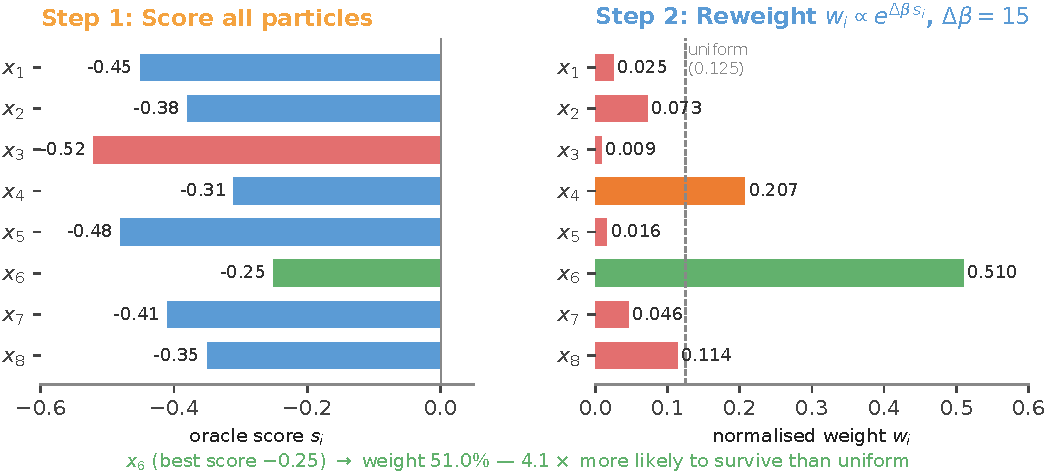
\includegraphics[width=0.95\linewidth]{figures/fig_gpa_walkthrough_score.pdf}
\caption{Score and reweight on the $N\!=\!8$ toy. \textbf{Left:} per-particle oracle scores $s_i$ (best in green: $x_6\!=\!-0.25$; worst in red: $x_3\!=\!-0.52$). \textbf{Right:} normalised weights after the tilt $w_i\!\propto\!\exp(\Delta\beta\,s_i)$ at $\Delta\beta\!=\!15$; uniform $1/N\!=\!0.125$ shown dashed. $x_6$ collects $51.0\%$ of the mass---$4.1\!\times$ the uniform expectation.}
\label{fig:walkthrough-score}
\end{figure}

\subsection{Adapting $\Delta\beta$ via bisection on $\ESS$}

The ESS-adaptive schedule (Lemma~\ref{lem:ess}) chooses $\Delta\beta_t$ so that $\ESS\!\geq\!\alpha N$ \emph{exactly} (not below). With $\alpha\!=\!0.5$, the target is $\ESS_{\rm target}\!=\!4$. Algorithm~\ref{alg:bisect} runs 64 bisection iterations on $[\Delta\beta_{\min}, \Delta\beta_{\max}]\!=\![0,1000]$.

\begin{algorithm}[h]
\caption{Bisection for $\Delta\beta$ given $\ESS$ target}\label{alg:bisect}
\begin{algorithmic}[1]
\State \textbf{Input:} scores $\{r_i\}_{i=1}^N$, target $\tau N$, range $[\Delta\beta_{\min}, \Delta\beta_{\max}]$, max iters $T_{\rm bs}$
\For{$t\!=\!1,\dots,T_{\rm bs}$}
    \State $\Delta\beta_{\rm mid}\!\leftarrow\!(\Delta\beta_{\min}+\Delta\beta_{\max})/2$
    \State $w_i\!\leftarrow\!\exp(\Delta\beta_{\rm mid}\,r_i)/Z$, with $Z\!=\!\sum_j\exp(\Delta\beta_{\rm mid}\,r_j)$
    \State $\ESS\!\leftarrow\!1/\sum_i w_i^2$
    \If{$\ESS > \tau N$} $\Delta\beta_{\min}\!\leftarrow\!\Delta\beta_{\rm mid}$ \Comment{can push harder}
    \Else \;$\Delta\beta_{\max}\!\leftarrow\!\Delta\beta_{\rm mid}$ \Comment{too aggressive}
    \EndIf
\EndFor
\State \textbf{Return:} $\Delta\beta_{\min}$
\end{algorithmic}
\end{algorithm}

For our example, the bisection converges to $\Delta\beta\!\approx\!11.7$, giving $\ESS\!\approx\!4.0\!=\!\alpha N$. The hand-picked $\Delta\beta\!=\!15$ above (which produced $\ESS\!=\!3.08$) was therefore more aggressive than the auto-schedule would choose.

\begin{figure}[h]
\centering
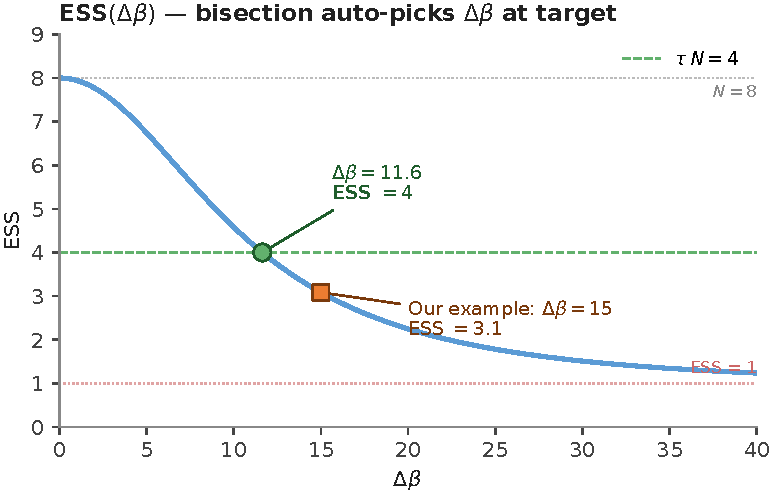
\includegraphics[width=0.78\linewidth]{figures/fig_gpa_walkthrough_ess.pdf}
\caption{$\ESS(\Delta\beta)$ for the $N\!=\!8$ toy oracle scores. The function decreases monotonically from $\ESS\!=\!N$ at $\Delta\beta\!=\!0$ toward $\ESS\!=\!1$ as $\Delta\beta\!\to\!\infty$ (winner-take-all). Bisection finds the unique $\Delta\beta\!=\!11.7$ at which $\ESS$ hits the target $\tau N\!=\!4$ (green dot). The hand-picked $\Delta\beta\!=\!15$ used in the walk-through (orange square) is past the target and so over-collapses the population.}
\label{fig:walkthrough-ess}
\end{figure}

\subsection{Resampling: multinomial vs.\ systematic}

\paragraph{Multinomial.} Draw counts $\!=\!(c_1,\dots,c_N)\!\sim\!\mathrm{Multinomial}(N, w)$. Expected copies per particle are $\E[c_i]\!=\!N\!\cdot\!w_i$, but the realised counts are noisy.

\paragraph{Systematic.} Lay the weights end-to-end as a unit interval $[0,1]$ (segment $i$ has width $w_i$). Drop $N$ pointers at positions $u\!+\!k/N$ for $k\!=\!0,\dots,N\!-\!1$, with $u\!\sim\!\mathrm{Uniform}[0,1/N)$. Particle $i$ receives a number of copies equal to the count of pointers in its segment. This has identical mean to multinomial but lower variance, and is the default in \gpa{}.

For our $N\!=\!8$ example with $u\!=\!0$, the eight pointers at $\{0.000, 0.125, 0.250, 0.375, 0.500, 0.625, 0.750, 0.875\}$ land in segments as follows: $w_2$ (cumulative 0.025--0.098) captures pointer 0.097; $w_4$ (0.107--0.314) captures pointers at 0.125, 0.250; $w_6$ (0.330--0.840) captures pointers at 0.375, 0.500, 0.625, 0.750; $w_8$ (0.886--1.000) captures pointer 0.875. Final copy counts:
\begin{center}
\begin{tabular}{lcccccccc}
\toprule
$i$       & 1 & 2 & 3 & 4 & 5 & 6 & 7 & 8 \\
copies    & 0 & 1 & 0 & 2 & 0 & 4 & 0 & 1 \\
\bottomrule
\end{tabular}
\end{center}
Four particles ($x^1, x^3, x^5, x^7$) are eliminated; $x^6$ is duplicated four times. After resampling, weights reset to $1/N\!=\!0.125$ uniformly.

\begin{figure}[h]
\centering
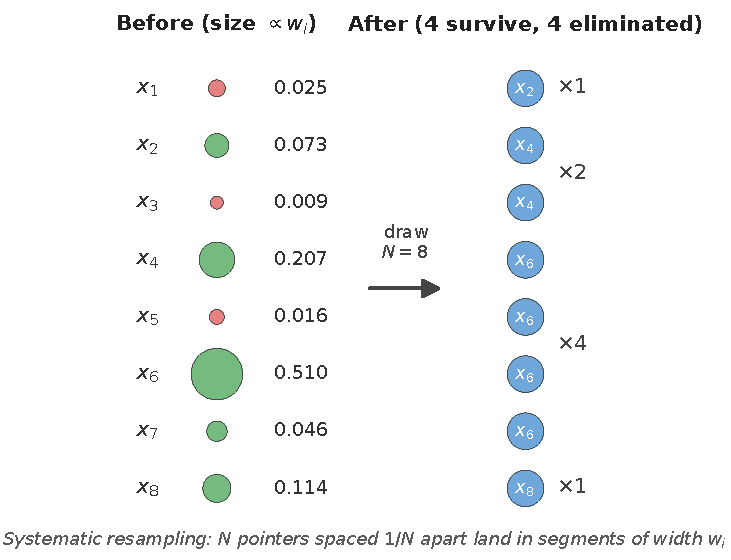
\includegraphics[width=0.85\linewidth]{figures/fig_gpa_walkthrough_resample.pdf}
\caption{Systematic resampling of the $N\!=\!8$ toy. \textbf{Left:} bubble area is proportional to $w_i$; green = retained, red = eliminated by the resampling step. \textbf{Right:} after resampling, all weights reset to $1/N$; $x_6$ now appears four times, $x_4$ twice, $x_2$ and $x_8$ once each. Four particles ($x_1, x_3, x_5, x_7$) are eliminated.}
\label{fig:walkthrough-resample}
\end{figure}

\subsection{Mutation: partial mask + denoise on a length-12 DNA toy}

Each of the eight resampled (now duplicate-rich) particles is independently mutated by $K_\beta$. Concretely, with mask fraction $\mathrm{nf}\!=\!0.25$ ($\!\to\!\lceil 0.25\!\cdot\!12\rceil\!=\!3$ positions on a length-12 sequence):
\begin{center}
\begin{tabular}{ll}
\toprule
\textbf{Step}        & \textbf{Sequence} \\
\midrule
Before (a duplicate of $x^6$)   & \texttt{ACGTATGCACGT} \\
Random mask 3 positions          & \texttt{AC?TA?GC?CGT} \\
Denoise via $p_\theta$           & \texttt{AC\textbf{T}TA\textbf{A}GC\textbf{A}CGT} \\
\midrule
Net edits                         & pos 3: G$\to$T; \, pos 6: T$\to$A; \, pos 9: C$\to$A \\
\bottomrule
\end{tabular}
\end{center}
Two properties this kernel inherits from the pretrained $p_\theta$:
\begin{itemize}
\item \emph{Grammar preservation.} The denoiser sees the unmasked context and proposes tokens consistent with whatever motif/composition rules $p_\theta$ has learned. Random per-position resampling would not.
\item \emph{Diversity restoration.} The four duplicates of $x^6$ each get an \emph{independent} random mask + denoising pass, so they diverge into four distinct child sequences. Without mutation the population would collapse to four identical copies.
\end{itemize}
The mask fraction $\mathrm{nf}$ controls exploration: $\mathrm{nf}\!=\!0.05$ is local search ($\sim\!10$ positions per step on a 200-bp DNA enhancer), $\mathrm{nf}\!=\!0.20$ is large jumps. Section~\ref{sec:results:ablation} reports sensitivity in the practical range.

%-----------------------------------------------------------------------
\section{Hyperparameters}\label{app:hyper}

Table~\ref{tab:hyper-rerd} lists hyperparameters for the SMC-protocol comparison (\drakes{} eval pair); Table~\ref{tab:hyper-ctrldna} lists those for \ctrldna{} comparison (HyenaDNA + gReLU MSE oracles); Table~\ref{tab:hyper-dnacraft} for \dnacraft{} comparison (HyenaDNA/DiMamba + Enformer 50/50). Default values are bolded.

\begin{table}[h]
\caption{Hyperparameters for the SMC-protocol comparison (HepG2 enhancer, MDLM backbone, \drakes{} split-oracle).}
\label{tab:hyper-rerd}
\centering
\small
\begin{tabular}{lll}
\toprule
Parameter & Mean recipe & Spec recipe \\
\midrule
$N$ (population) & 5000 & 5000 \\
$\alpha$ (ESS threshold) & 0.5 & 0.5 \\
$\beta_*$ (target inverse temp) & 200 & 100 \\
$T_{\max}$ (max steps) & 30, hard cap 200 & 30, hard cap 200 \\
nf (mask fraction) & 0.05 & 0.05 \\
DPS gradient strength $\eta$ & 3000 & 3000 \\
$\mathrm{pw}$ (off-target penalty) & 0 & 0.35 \\
GC bio-filter & [0.45, 0.55] & [0.45, 0.55] \\
\bottomrule
\end{tabular}
\end{table}

\begin{table}[h]
\caption{Hyperparameters for \ctrldna{} comparison (Reddy promoters, HyenaDNA backbone, gReLU MSE oracles, universal recipe).}
\label{tab:hyper-ctrldna}
\centering
\small
\begin{tabular}{ll}
\toprule
Parameter & Universal recipe \\
\midrule
$N$ (population) & 10000 \\
$\alpha$ (ESS threshold) & 0.5 \\
$\beta_*$ & 100 \\
$T_{\max}$ (steps) & 60 \\
nf (mask fraction) & 0.05 \\
$K$ (branch factor) & 8 \\
$\mathrm{pw}$ & 0.35 \\
diversity $\lambda$ (conformity) & \textbf{1.0} \\
DPS & off \\
GC bio-filter & off \\
\bottomrule
\end{tabular}
\end{table}

\begin{table}[h]
\caption{Hyperparameters for \dnacraft{} comparison (Gosai 50/50 split, top-128 by MinGap-Eval). C1 = no GC penalty; C3 = soft GC penalty (gct=0.60), no hard bio-filter.}
\label{tab:hyper-dnacraft}
\centering
\small
\begin{tabular}{lll}
\toprule
Parameter & C1 & C3 \\
\midrule
$N$ (population) & 5000 & 5000 \\
$\beta_*$ & 25 & 25 \\
$\mathrm{pw}$ & 0.30 & 0.30 \\
DPS & on & on \\
GC penalty (gct) & --- & 0.60 \\
GC bio-filter & off & off \\
$K$ & 8 & 8 \\
\bottomrule
\end{tabular}
\end{table}

%-----------------------------------------------------------------------
\section{Full GPA-vs-ISM/LEDIDI tables}\label{app:ism_full}

Single-sequence comparison: GPA row = the one sequence in each pool that maximises $\mathrm{AG}-\mathrm{LN}$ (sweet spot: low LN, high held-out AG). Directly comparable to \ism{}/\ledidi{} which are inherently single-sequence.

\begin{table}[h]
\caption{Single-sequence comparison, K562 enhancer, two seeds (uid=181692 natural, uid=50178 random). \gpa{} row = argmax of $\mathrm{AG}-\mathrm{LN}$ within the 5{,}000-seq pool.}
\label{tab:ism_singleseq}
\centering
\small
\begin{tabular}{llrrr}
\toprule
Seed & Method & Edits & LN & AG \\
\midrule
\multirow{4}{*}{uid=181692}
 & \gpa{} (no DPS) uncap   &  96 & 4.97 & \textbf{3.33} \\
 & \gpa{} (+DPS) cap30     &  60 & 6.21 & \textbf{3.47} \\
 & \ism{} gen 115          & 115 & 8.74 & 2.83 \\
 & \ledidi{} t15 $\lambda$=0.05 & 125 & 9.81 & $-$0.22 \\
\midrule
\multirow{4}{*}{uid=50178}
 & \gpa{} (no DPS) cap30   &  60 & 4.71 & 2.75 \\
 & \gpa{} (+DPS) cap30     &  59 & 6.58 & \textbf{3.61} \\
 & \ism{} gen 115          & 115 & 9.58 & 2.92 \\
 & \ledidi{} t15 $\lambda$=0.05 & 105 &11.66 & $-$0.62 \\
\bottomrule
\end{tabular}
\end{table}

\paragraph{Reading the table.}
A single \gpa{} sequence (e.g.\ +DPS cap30 on uid=50178: LN $6.58$, AG $3.61$) beats \ism{} gen 115 on the held-out AG by $+0.69$ at LN $\sim\!3.0$ lower—better held-out activity \emph{and} less reward-hacking. Under any selection rule, \ledidi{} stays AG-negative; not one of its 50 reruns produces an AG-positive sequence.

\paragraph{Apples-to-apples runtime (single H100, K562 enhancer, 5{,}000-sequence pool).}
Table~\ref{tab:ism_runtime} reports wall-time at matched output volume, averaged across the random and natural pools. \gpa{} is fully population-parallel: a single SMC step propagates all 5{,}000 particles together through the diffusion proposal, so the per-particle cost is the GPU-memory chunk \texttt{mutation\_batch\_size=128} amortised over the population. \ism{} is also nominally population-parallel (5{,}000 independent greedy trajectories), but its sequential cost is fixed at 115 generations per seed, and that dominates wall regardless of how memory chunks are batched. \ledidi{} is chunked-sequential by design: 5{,}000 seeds processed in 39 chunks of 128 along the Gumbel-softmax optimisation. The result is $\sim\!9.3\times$ speedup over \ism{} and $\sim\!3.4\times$ speedup over \ledidi{} at identical pool size and identical hardware.

\begin{table}[h]
\caption{Apples-to-apples runtime: single H100, 5{,}000-sequence K562-enhancer pool, averaged across random and natural seed pools. \gpa{} = v3 noDPS recipe (matches Sec.~\ref{sec:results:ism}). Speedup column is $\mathrm{wall}_{\text{baseline}}/\mathrm{wall}_{\gpa{}}$.}
\label{tab:ism_runtime}
\centering
\small
\begin{tabular}{lllr}
\toprule
Method & Wall (5K pool) & Parallelism & Speedup vs.\ \gpa{} \\
\midrule
\textbf{\gpa{}} & \textbf{$\sim\!11.6$ min} & population-parallel (5{,}000 SMC particles) & --- \\
\ledidi{}       & $\sim\!40$ min     & chunked-sequential (39 chunks $\times$ 128 seeds) & $\sim\!3.4\times$ slower \\
\ism{}          & $\sim\!107.5$ min  & population-parallel, but 115 sequential greedy gens & $\sim\!9.3\times$ slower \\
\bottomrule
\end{tabular}
\end{table}

%-----------------------------------------------------------------------
\section{Full DNA-CRAFT tables (GPA-C1 vs GPA-C3)}\label{app:dnacraft_full}

The headline column in Table~\ref{tab:dnacraft} uses GPA-C3 (\texttt{dps\_pw030\_b25\_gct060\_nobio}). This appendix shows the same benchmark with the alternate recipe variant GPA-C1 (\texttt{dps\_pw030\_b25}, no GC penalty), under the matched-output-budget protocol of Table~\ref{tab:dnacraft} (\texttt{by\_pool\_composite} top-64 from \texttt{gpa\_output\_best\_eval.h5}, 3 reps for both variants). Both variants run at $\sim\!3.6$ min/seed (no MCTS) on the MDLM backbone; the only difference is the soft GC-centering term added to C3's DPS gradient.

\paragraph{Recipe decomposition.}
Each token in the recipe name maps to a specific knob in the GPA algorithm of \S\ref{sec:method}, with no other differences between the two variants:
\begin{itemize}
\item \texttt{dps} -- enables the Gumbel-softmax oracle gradient with strength $\eta\!=\!3000$ (\S\ref{sec:method:ext}, ``Gumbel-softmax oracle gradient (DPS)''). This is a biased proposal in the sense of \S\ref{sec:method:ext} and is shared by both C1 and C3, so the C1$\leftrightarrow$C3 contrast does not move along the DPS-bias axis.
\item \texttt{pw030} -- sets the off-target weight $\mathrm{pw}\!=\!0.30$ in the linear fitness of Eq.~\ref{eq:fitness} (\S\ref{sec:method:pw}); the same $0.30$ weights the off-target term inside the DPS gradient as well.
\item \texttt{b25} -- sets the SMC tilt ceiling $\beta_*\!=\!25$. This is below the default range $\beta_*\!\in\!\{100,200\}$ in \S\ref{sec:exp} and is a deliberately gentler tilt that preserves population diversity at some cost in MinGap; both variants share it.
\item \texttt{gct060} \emph{(C3 only)} -- adds a quadratic centering term $-w\,(g(x)-0.60)^2$ to the DPS objective before backpropagation, where $g(x)\!=\!\overline{P(C)+P(G)}$ is the per-position soft-onehot GC fraction and $w\!=\!10$. The penalty rides inside the same Gumbel-softmax gradient that DPS already computes; it is \emph{not} a hard accept/reject filter.
\item \texttt{nobio} -- disables the hard bio-filter (no \texttt{gc\_low}/\texttt{gc\_high} interval gating). All GC discipline in C3 therefore comes from the soft \texttt{gct060} term in the DPS gradient.
\end{itemize}
Both variants additionally use the default branch factor $K\!=\!8$ (\S\ref{sec:method:ext}, Prop.~\ref{prop:K}) and population $N\!=\!5{,}000$ (Table~\ref{tab:dnacraft} caption), so both target $\pi_{\beta_*}^{(K=8)}\!\neq\!\pi_{\beta_*}$ in the sense of Prop.~\ref{prop:K}; the C1$\leftrightarrow$C3 contrast isolates the GC-centering term with $K$, $\beta_*$, $\mathrm{pw}$, $N$, and the DPS bias all held constant.

\begin{table}[h]
\caption{\dnacraft{} benchmark with the GPA-C1 alternate recipe (\texttt{dps\_pw030\_b25}; no GC penalty), reported alongside the headline GPA-C3 (Table~\ref{tab:dnacraft}). Both columns: \texttt{by\_pool\_composite} top-64 from \texttt{gpa\_output\_best\_eval.h5}, mean (std) over 3 reps. Baselines verbatim from \citet{dnacraft2026}.}
\label{tab:dnacraft_full_eval}
\centering
\scriptsize
\begin{tabular}{llcccccccccc}
\toprule
Cell & Metric & SMC & CG & TDS & DRAKES & D3 & Ledidi & Ctrl-DNA & DNA-CRAFT & \gpa{}-C1 & \gpa{}-C3 \\
\midrule
\multirow{4}{*}{HepG2}
 & MinGap   & 1.61 & $-$0.23 & 0.40 & $-$1.40 & 0.05 & 5.77 & \textbf{7.79} & 4.35 & 6.87 & 6.91 \\
 & Motif    & 0.55 & 0.86 & 0.40 & 0.06 & 0.87 & 0.58 & 0.63 & \textbf{0.92} & 0.90 & \textbf{0.92} \\
 & 3-mer    & 0.81 & 0.97 & 0.74 & $-$0.36 & \textbf{0.98} & 0.76 & 0.49 & \textbf{0.98} & 0.95 & 0.95 \\
 & Diversity& 0.83 & \textbf{1.98} & 0.96 & 1.86 & \textbf{1.98} & \textbf{1.98} & 1.90 & \textbf{1.98} & 1.81 & 1.86 \\
\midrule
\multirow{4}{*}{K562}
 & MinGap   & 4.12 & 0.00 & 1.62 & $-$0.20 & 0.18 & 7.66 & \textbf{9.07} & 5.69 & 8.18 & 8.13 \\
 & Motif    & 0.45 & 0.85 & 0.51 & 0.14 & 0.86 & 0.65 & 0.63 & 0.93 & 0.93 & \textbf{0.94} \\
 & 3-mer    & 0.66 & 0.94 & 0.65 & $-$0.35 & 0.96 & 0.69 & 0.41 & \textbf{0.98} & 0.92 & 0.95 \\
 & Diversity& 0.31 & \textbf{1.98} & 0.64 & 1.96 & \textbf{1.98} & \textbf{1.98} & 1.90 & \textbf{1.98} & 1.56 & 1.83 \\
\midrule
\multirow{4}{*}{SK-N-SH}
 & MinGap   & 0.56 & $-$0.28 & 0.19 & 0.09 & $-$0.01 & 3.03 & 3.72 & 3.23 & \textbf{5.07} & 4.98 \\
 & Motif    & 0.52 & 0.86 & 0.48 & 0.23 & 0.84 & 0.38 & 0.48 & 0.88 & 0.89 & \textbf{0.92} \\
 & 3-mer    & 0.78 & 0.95 & 0.72 & $-$0.38 & 0.93 & 0.37 & 0.20 & \textbf{0.97} & 0.87 & 0.94 \\
 & Diversity& 1.27 & \textbf{1.98} & 0.92 & 1.83 & 1.97 & \textbf{1.98} & 1.86 & \textbf{1.98} & 1.59 & 1.86 \\
\bottomrule
\end{tabular}
\end{table}

\paragraph{Reading.}
GPA-C1 and GPA-C3 give nearly tied MinGap and Motif Spearman on every cell (within seed std on most rows). C3 wins Motif on HepG2 / K562 / SK-N-SH ($+0.02$/$+0.01$/$+0.03$) and 3-mer on K562 / SK-N-SH ($+0.03$/$+0.07$). The biggest practical difference is Diversity: the soft GC-centering term in C3's DPS gradient recovers $+0.05$ to $+0.27$ Shannon bits over C1 on every cell, lifting C3 above the Ctrl-DNA Diversity floor on all three cells. The mechanism is indirect: by penalising drift away from $g(x)\!=\!0.60$ at every Gumbel-softmax step, the term blunts the oracle's tendency to push particles toward narrow high-GC modes, which in turn keeps the population spread out in sequence space. C1 wins MinGap on K562 / SK-N-SH ($+0.05$/$+0.09$) but loses across the rest. C3 is the headline because the +Diversity / +Motif / +3-mer trade dominates the small MinGap give-back; C1 is reported as an ablation that isolates the GC-penalty's contribution.

\paragraph{Backbone caveat.}
\dnacraft{}'s reported numbers in Table~\ref{tab:dnacraft} are obtained on a Mamba-style discrete-diffusion (DiMamba) backbone whose code and pretrained checkpoints are not publicly available; the same paper also reports DiMamba-vs-MDLM ablations that show DiMamba contributes additional biological-faithfulness gains. Our \gpa{}-C1 / \gpa{}-C3 numbers are obtained on the publicly available MDLM backbone of \citet{sahoo2024mdlm} and should be read as a lower bound on what \gpa{} would achieve at backbone parity, by Remark~\ref{rem:agnostic}.

%-----------------------------------------------------------------------
\section{Wall-time table}\label{app:wall}

\begin{table}[h]
\caption{Wall time per seed and 5-seed totals (HepG2, identical H100 hardware, identical HyenaDNA backbone). Wall time excludes downstream motif scoring.}
\label{tab:wall}
\centering
\small
\begin{tabular}{lrr}
\toprule
Method & Wall/seed (h) & 5-seed total (GPU-h) \\
\midrule
\ctrldna{} R200 (RL fine-tune) & $43.5\pm 0.8$ & $\sim\!218$ \\
\gpa{} v3 (K=8, no diversity)  & $3.97\pm 0.59$ & 19.8 \\
\gpa{} v4 (K=8 + rejuvenation) & $2.17\pm 0.22$ & 10.8 \\
\gpa{} v5 (K=8 + diversity)    & $\mathbf{2.22\pm 0.52}$ & $\mathbf{11.1}$ \\
\bottomrule
\end{tabular}
\end{table}

%-----------------------------------------------------------------------
\section{DPS gradient ablation}\label{app:dps_ablation}

Population annealing alone (no DPS) already beats single-chain refinement baselines; DPS gradient is a multiplicative enhancement.

\begin{table}[h]
\caption{DPS gradient ablation on Gosai HepG2.}
\label{tab:dps_ablation}
\centering
\small
\begin{tabular}{llrrr}
\toprule
Track & Metric & \gpa{}-only & \gpa{}+DPS & $\Delta$(DPS) \\
\midrule
Mean & $H_{\mathrm{eval}}$ & $8.73\pm 0.50$ & $\mathbf{10.06\pm 0.19}$ & $+1.33$ \\
Mean & Spec & 1.58 & 3.06 & $+1.48$ \\
Spec & $H_{\mathrm{eval}}$ & $8.28\pm 0.12$ & $9.35\pm 0.20$ & $+1.07$ \\
Spec & Spec & $6.11\pm 1.45$ & $\mathbf{7.61\pm 0.25}$ & $+1.50$ \\
\bottomrule
\end{tabular}
\end{table}

%-----------------------------------------------------------------------
\section{Naturalness audit}\label{app:naturalness}

\begin{table}[h]
\caption{Naturalness audit (HepG2 top-128). \gpa{} produces bio-plausible sequences by construction; \ctrldna{} reward-hacks to non-biological space.}
\label{tab:nat}
\centering
\small
\begin{tabular}{lrrr}
\toprule
Metric & Real (Gosai) & \gpa{} & \ctrldna{} \\
\midrule
GC mean & 0.44 & 0.41 & 0.45 \\
\textbf{bio\_pass\_rate} & 0.51 & $\mathbf{1.00}$ & $\mathbf{0.05}$ \\
max homopolymer & 5.4 & 5.1 & $\mathbf{20.9}$ \\
$k$=3 Pearson & 1.0 & 0.61 & 0.39 \\
HNF1A enrichment & $0\times$ & $10\,040\times$ & $7\,812\times$ \\
\bottomrule
\end{tabular}
\end{table}

\begin{figure}[h]
\centering
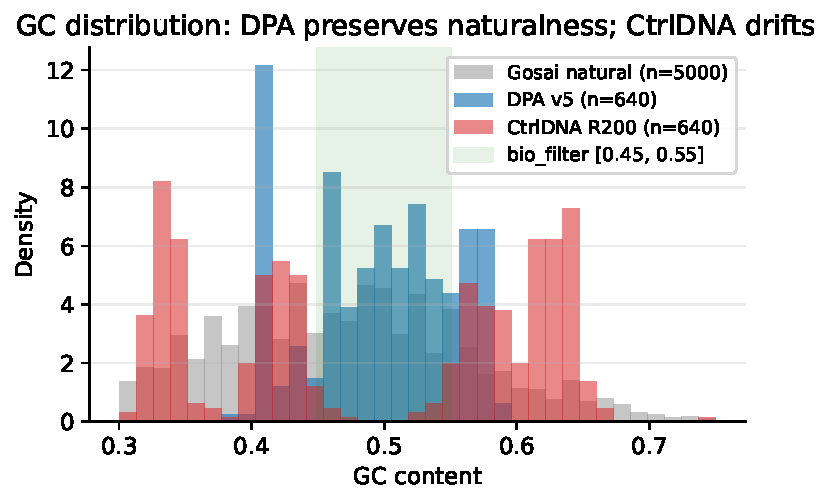
\includegraphics[width=0.6\linewidth]{figures/fig2_gc.pdf}
\caption{GC distribution comparison on HepG2 top-128 sequences. \gpa{} (blue) clusters near the lower edge of the bio-filter (45\%) but stays within the natural Gosai range (gray); \ctrldna{} (red) drifts widely, with a heavy tail of low- and high-GC sequences and a substantial fraction outside the natural distribution.}
\label{fig:gc}
\end{figure}

%-----------------------------------------------------------------------
\section{Extreme specificity}\label{app:extreme}

Pushing $\mathrm{pw}$ beyond the canonical $0.35$ trades $H_{\mathrm{eval}}$ for higher specificity until both off-targets fall below baseline (Table~\ref{tab:extreme}).

\begin{table}[h]
\caption{Extreme-specificity extension on Gosai HepG2 (single run each, $N\!=\!5000$).}
\label{tab:extreme}
\centering
\small
\begin{tabular}{rrrrr}
\toprule
$\mathrm{pw}$ & $H_{\mathrm{eval}}$ & $K_{\mathrm{eval}}$ & $S_{\mathrm{eval}}$ & $H{>}8 \wedge K{<}0 \wedge S{<}0$ \\
\midrule
0.35 & 9.65 & 2.15 &  1.10 & 0 \\
0.50 & 9.54 & 1.96 &  0.63 & 0 \\
0.70 & 8.73 & 1.52 &  0.35 & 0 \\
1.00 & 8.57 & 0.69 & $-$0.48 & 26 \\
1.50 & $\mathbf{8.44}$ & 0.55 & $\mathbf{-0.66}$ & $\mathbf{54}$ \\
\bottomrule
\end{tabular}
\end{table}

\paragraph{Beta trajectory.}
Figure~\ref{fig:beta} shows a representative ESS-adaptive $\beta$ trajectory and the population-mean reward over SMC steps for a HepG2 run.

\begin{figure}[h]
\centering
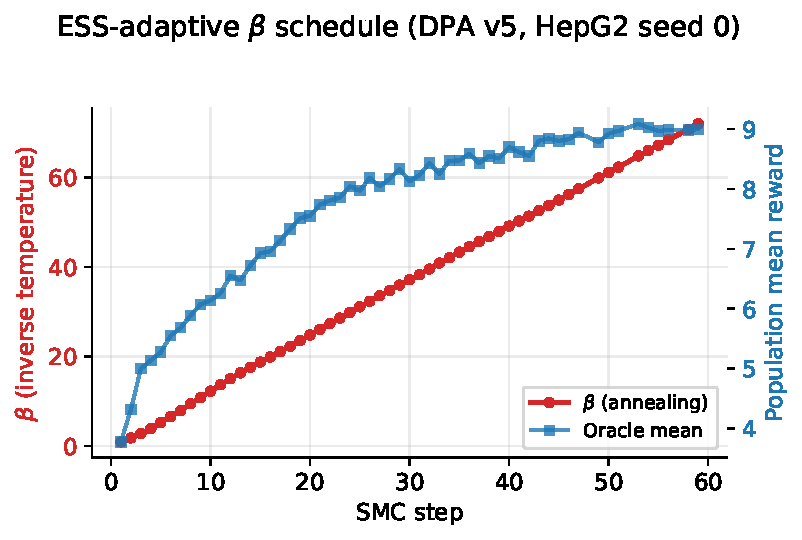
\includegraphics[width=0.6\linewidth]{figures/fig4_beta_traj.pdf}
\caption{Representative \gpa{} run trajectory (HepG2, seed 0). Red trace: ESS-adaptive $\beta$ schedule rises through the annealing path. Blue trace: population mean reward grows monotonically toward saturation as $\beta$ increases.}
\label{fig:beta}
\end{figure}

%-----------------------------------------------------------------------
\section{Negative result: APF correction for $\epsilon$-greedy $K$-branching}\label{app:apf}

A natural attempt to recover Shannon under $K$-branching is to soften the argmax with $\epsilon$-greedy ($\tau\!>\!0$ softmax over the $K$ siblings) and apply the auxiliary-particle-filter weight correction \citep{pittshephard1999}:
\[
w_{\mathrm{new}} = w_{\mathrm{old}}\big/p_\tau(\mathrm{winner}),\qquad p_\tau(j)=\exp(r_j/\tau)\big/\sum_m\exp(r_m/\tau).
\]
Compute the expectation:
\[
\E[w_{\mathrm{new}}\,\varphi(x_{\mathrm{winner}})] = \E_{x_{1:K}\sim q}\!\!\left[\sum_{j=1}^K \frac{\exp(r_j/\tau)}{\sum_m\exp(r_m/\tau)}\cdot\frac{\sum_m\exp(r_m/\tau)}{K\exp(r_j/\tau)}\,\varphi(x_j)\right]=\frac{1}{K}\sum_j \E_q[\varphi(x_j)],
\]
i.e.\ the corrected estimator is equivalent to a single-child sample. The $K$ siblings collapse and the effective-$\beta$ boost vanishes. Empirically, on a synthetic linear reward $r(x)\!=\!3x$ with $q$ uniform on $[0,1]$ (200K Monte-Carlo trials):
\begin{center}
\small
\begin{tabular}{lrrr}
\toprule
Variant & $\E[x]$ & $\mathrm{Var}[x]$ & ESS \\
\midrule
$K=1$ no selection                & 0.5000 & 0.0833 & 100.0\% \\
$K=8$ argmax (no correction)      & 0.8887 & 0.0099 & 100.0\% \\
$K=8$ softmax $\tau\!=\!0.3$ (no corr.) & 0.8445 & 0.0180 & 100.0\% \\
\textbf{$K=8$ softmax $\tau\!=\!0.3$ + APF} & 0.4880 & 0.0874 & 0.4\% \\
$K=8$ softmax $\tau\!=\!1.0$ + APF & 0.5009 & 0.0829 & 53.1\% \\
\bottomrule
\end{tabular}
\end{center}
ESS collapses at low $\tau$ and the corrected mean/variance reproduces $K=1$. We therefore do \emph{not} use APF correction for production runs and report only argmax $K$-branching. K-annealing schedules and waste-free SMC \citep{dau2022wastefree} remain valid theoretical alternatives, deferred to future work.

%-----------------------------------------------------------------------
\section{Negative result: post-hoc Metropolis tempering}\label{app:posthoc}

Another natural Shannon-rescue move is to load the concentrated argmax-$K$ pool and run Metropolis–Hastings at lower $\beta'$ to spread the population. We tested this on the K562 promoter pool (50 MH steps, nf=0.05, HyenaDNA proposal):

\begin{center}
\small
\begin{tabular}{rrrrr}
\toprule
$\beta'$ & accept rate & $\Delta$comp & $\Delta$tgt & $\Delta H$ \\
\midrule
25 &  3.4\% & $+0.02$ & $-0.06$ & $+0.05$ \\
12 &  6.5\% & $-0.15$ & $-0.27$ & $+0.10$ \\
 6 & 13.1\% & $-0.68$ & $-0.77$ & $+0.21$ \\
 3 & 29.1\% & $-2.12$ & $-2.22$ & $+0.39$ \\
 1 & 73.7\% & $-4.71$ & $-5.35$ & $+0.61$ \\
\bottomrule
\end{tabular}
\end{center}
The Pareto slope is $\sim\!3\!-\!5$ target units per $0.1$ nat of Shannon, far too steep for the diversity gap to \dnacraft{}/\ctrldna{} K562 ($\sim\!0.5$ nat) to be closed without erasing the target advantage. Increasing chain length or shrinking nf does not change the local-neighborhood geometry. The honest reading: under sharply peaked oracles, the activity–diversity tension is in the reward landscape, not the sampler.

%-----------------------------------------------------------------------
\section{GC distribution and floor-hugging}\label{app:gc}

Even with the bio-filter $\mathrm{GC}\!\in\![0.45,0.55]$, $60\!-\!75\%$ of \gpa{} top-128 sequences cluster at the lower bound. Two facts:
\begin{enumerate}
\item This is a property of the \emph{masked-diffusion proposal} at low noise fraction. At $\mathrm{nf}\!=\!0.20$ the bias inverts toward the upper bound (GC $\approx\!0.54$); the crossover occurs near $\mathrm{nf}\!\approx\!0.16\!-\!0.17$.
\item The eval oracle is GC-agnostic: at both $\mathrm{nf}$ extremes, top-128 oracle scores are comparable. The GC bias arises from $p_\theta$, not from the reward signal.
\end{enumerate}
Three mitigations were tested with mixed success: (i) GC-aware DPS gradient (\verb|gc_dps_weight|) reduces floor-hugging from $61.5\%$ to $55.0\%$ at $-0.09$ $H_{\mathrm{eval}}$ cost; (ii) narrow $1\%$ GC bands achieve uniform GC by construction at $-0.25$ $H_{\mathrm{eval}}$; (iii) stratified resampling within $2\%$ GC bins \citep{verge2015island} achieves balanced coverage at $-0.50$ to $-1.0$ $H_{\mathrm{eval}}$. We report all three options in the codebase but use the unmitigated baseline in the headline tables for fair comparison with peer methods.

%-----------------------------------------------------------------------
\section{Ctrl-DNA enhancer comparison (V7 main + V5/V8 ablations)}\label{app:ctrldna_enhancer}

This appendix gives the dedicated \ctrldna{}-vs-\gpa{} enhancer comparison referenced in \S\ref{sec:results:promoter}. Same Gosai 50/50 split as the \dnacraft{} benchmark, top-128 selection per cell, 5 \gpa{} seeds. The headline GPA recipe is V7 (universal: $K\!=\!8$, diversity $\lambda\!=\!1.0$); V8a, V8b (alternative pairwise-suppression formulations) and V5 (the previous default with $\lambda\!=\!0.2$) are ablations.

\begin{table}[h]
\caption{Ctrl-DNA vs.\ \gpa{} on Gosai HepG2/K562/SKNSH enhancers (5 seeds; mean (std)). Headline = V7 universal recipe; V8a (log\_ratio + pw=1.0), V8b (linear + pw=1.0) and V5 ($\lambda\!=\!0.2$) are ablations of the diversity / pairwise-suppression knob. \texttt{target\_raw} = mean target oracle score; \texttt{ΔR} = normalised target minus mean off-target; \texttt{shannon} = per-position entropy; \texttt{motif\_corr} = FIMO Pearson against per-cell real reference.}
\label{tab:ctrldna_enhancer}
\centering
\footnotesize
\setlength{\tabcolsep}{4pt}
\begin{tabular}{llrrrr}
\toprule
Cell & Method & target\_raw $\uparrow$ & ΔR $\uparrow$ & shannon $\uparrow$ & motif\_corr $\uparrow$ \\
\midrule
\multirow{5}{*}{HepG2}
 & \ctrldna{} R200             & 5.32 (0.65) & 0.48 (0.10) & 1.65 (0.14) & \textbf{0.29} (0.16) \\
 & \gpa{} V5 ($K\!=\!8, \lambda\!=\!0.2$) & 9.86 (0.10) & 0.85 (0.01) & 1.49 (0.03) & 0.19 (0.03) \\
 & \gpa{} V7 ($K\!=\!8, \lambda\!=\!1.0$) & \textbf{9.90} (0.12) & 0.84 (0.02) & 1.59 (0.11) & 0.20 (0.02) \\
 & \gpa{} V8a (log\_ratio, pw=1.0) & 6.61 (0.04) & 0.68 (0.01) & \textbf{1.93} (0.00) & 0.15 (0.02) \\
 & \gpa{} V8b (linear, pw=1.0) & 9.51 (0.10) & \textbf{0.93} (0.02) & 1.70 (0.11) & 0.10 (0.04) \\
\midrule
\multirow{5}{*}{K562}
 & \ctrldna{} R200             & \textbf{9.99} (1.52) & \textbf{0.77} (0.14) & 1.60 (0.15) & 0.24 (0.07) \\
 & \gpa{} V5 ($K\!=\!8, \lambda\!=\!0.2$) & 8.82 (0.13) & 0.34 (0.00) & 1.43 (0.09) & \textbf{0.26} (0.02) \\
 & \gpa{} V7 ($K\!=\!8, \lambda\!=\!1.0$) & 8.83 (0.12) & 0.32 (0.01) & 1.65 (0.02) & 0.24 (0.02) \\
 & \gpa{} V8a (log\_ratio, pw=1.0) & 6.48 (0.03) & 0.39 (0.01) & \textbf{1.94} (0.01) & 0.24 (0.01) \\
 & \gpa{} V8b (linear, pw=1.0) & 8.15 (0.04) & 0.41 (0.01) & 1.68 (0.02) & 0.25 (0.02) \\
\midrule
\multirow{5}{*}{SK-N-SH}
 & \ctrldna{} R200             & 9.93 (1.13) & \textbf{0.71} (0.10) & 1.63 (0.17) & \textbf{0.23} (0.10) \\
 & \gpa{} V5 ($K\!=\!8, \lambda\!=\!0.2$) & \textbf{14.33} (0.20) & 0.10 (0.01) & 1.49 (0.04) & \textbf{0.23} (0.01) \\
 & \gpa{} V7 ($K\!=\!8, \lambda\!=\!1.0$) & 14.17 (0.18) & 0.10 (0.00) & 1.63 (0.04) & 0.20 (0.01) \\
 & \gpa{} V8a (log\_ratio, pw=1.0) & 6.29 (0.08) & 0.22 (0.01) & \textbf{1.91} (0.01) & 0.15 (0.01) \\
 & \gpa{} V8b (linear, pw=1.0) & 8.26 (0.15) & 0.29 (0.03) & 1.74 (0.05) & 0.10 (0.01) \\
\bottomrule
\end{tabular}
\end{table}

\paragraph{Headlines.}
\gpa{} V7 (the universal recipe) wins target\_raw on HepG2 and SK-N-SH ($+4.58$ and $+4.24$ over \ctrldna{}), and is competitive on K562 within $\sim$1 std. \ctrldna{} retains a ΔR (specificity) edge on K562 and SK-N-SH at the cost of $\sim$50\% lower target activity on HepG2/SK-N-SH and high seed-to-seed variance ($\pm 1.13$--$1.52$). The V7 vs.\ V5 comparison shows the diversity-$\lambda$ bump (from $0.2$ to $1.0$) buys $+0.10$--$0.22$ shannon on every cell at zero target cost, isolating the population-conformity penalty as a strict Pareto improvement. V8a/V8b are alternative pairwise-suppression formulations: V8a (log-ratio reward, pw=1.0) achieves the tightest shannon ($1.91$--$1.94$, near uniform) but at substantial target cost; V8b (linear, pw=1.0) recovers HepG2/K562 target while maximising HepG2 ΔR. The four GPA variants together trace a Pareto front in (target, shannon, motif) space at fixed inference cost---one knob per recipe, no retraining.

%-----------------------------------------------------------------------
\section{DNA-CRAFT $K$ and $i$ scaling sweeps (UCB-MCTS variant)}\label{app:ucb_scaling}

\paragraph{Why MCTS at all.}
DNA-CRAFT replaces the SMC population with a single depth-bounded Monte Carlo Tree Search loop on a DiMamba diffusion backbone, and shows that this delivers state-of-the-art motif and 3-mer grammar fidelity on the Gosai enhancer benchmark (Table~\ref{tab:dnacraft}). The mechanism that delivers their grammar bar is plausible on its face: tree search amortises the cost of choosing the right next mutation by replaying the same scoring oracle across multiple competing children before committing—a strictly more informed proposal than picking the first child that scores well. \gpa{}'s standard $K$-branch is a depth-1 special case of this idea: try $K$ candidates from the proposal and keep the best (Sec.~\ref{sec:method:ext}). It is natural to ask whether the same \emph{deeper} planning that powers \dnacraft{}'s grammar—expanding the best leaves over multiple iterations rather than just one---closes \gpa{}'s residual gap to \dnacraft{} on motif/3-mer correlation. The \texttt{ucb\_stacked} variant exists to test exactly that question.

\paragraph{What \texttt{ucb\_stacked} does, step by step.}
At every SMC mutation step, each particle $x_t^{(j)}$ becomes the root of an independent Monte Carlo tree. We then run $i$ iterations on that tree, where each iteration follows the standard four-phase MCTS-with-UCB1 loop \citep[``UCT'';][]{kocsis2006uct}:
\begin{enumerate}
\item \emph{Selection.} Traverse from the root to a leaf by greedily picking, at each internal node $v$ with already-expanded children $\{a\}$, the child that maximises the UCB1 score \citep{auer2002ucb,kocsis2006uct}
\begin{equation}\label{eq:ucb1}
    \mathrm{UCB1}(a) \;=\; \bar{Q}(a) \;+\; c\sqrt{\frac{\ln n(v)}{n(a)}},
\end{equation}
where $\bar{Q}(a)\!\in\![0,1]$ is the mean (range-normalised) reward backed up through child $a$, $n(a)$ is the visit count of $a$, $n(v)\!=\!\sum_a n(a)$ is the parent visit count, and $c\!=\!\sqrt{2}$ is the standard exploration constant. The first term exploits children with high empirical value; the second term explores low-visit children with a $\sqrt{\log n / n(a)}$ confidence radius. Together this is the canonical bandit rule of \citet{auer2002ucb} for stochastic multi-armed bandits, and \citet{kocsis2006uct} show that applying it node-wise inside a tree (UCT) inherits the same $\mathcal{O}(\log n)$ regret bound at each node. Children with $n(a)\!=\!0$ are tried first by convention so the second term remains well-defined.
\item \emph{Expansion.} Apply \gpa{}'s standard $K$-branch operator at the selected leaf: draw $K\!=\!8$ children using partial-mask$\circ$denoise + DPS (the same operator the no-MCTS \gpa{} would use as its mutation kernel).
\item \emph{Evaluation.} Score each new child under the eval-side reward.
\item \emph{Backpropagation.} Update visit counts $n(\cdot)$ and value estimates $\bar{Q}(\cdot)$ along the path from each new child up to the root, so the next iteration's UCB1 selection (Eq.~\ref{eq:ucb1}) uses fresh statistics.
\end{enumerate}
We bound the tree depth at $d\!=\!2$, so the planner looks at most two mutation steps ahead. After $i$ iterations the tree has at most $1\!+\!i\!\cdot\!K$ nodes; the mutated state for $x_t^{(j)}$ is the highest-reward leaf in that tree. The SMC step then proceeds as usual: the new particle states are importance-weighted at the next $\beta$, resampled if $\ESS$ degenerates, and the loop continues.

\paragraph{Connection to \dnacraft{}.}
The four-step loop (UCB selection $\to$ $K$-fold expansion $\to$ scoring $\to$ reward backprop) is identical in shape to \dnacraft{}'s tree search. What differs is the \emph{scope} of where the tree sits and how it is consumed:
\begin{itemize}
\item \dnacraft{} runs \emph{one} MCTS for the whole design problem: $N_{\mathrm{iter}}\!=\!64$ iterations, $M\!=\!128$ children per expansion, full leaf-to-clean rollouts. Their MinGap-Set archive accumulates the best $N_{\max}\!=\!64$ leaves seen during the run, and that archive is the output (no SMC, no population).
\item \texttt{ucb\_stacked} runs \emph{many} MCTSs: one per particle, per SMC step. Each tree is run for $i\!\in\!\{12,18,24,36\}$ iterations with $K\!=\!8$ children per expansion at depth $d\!=\!2$, no full rollouts (we score after one denoising step). The output is the SMC population at the final $\beta$, exactly as in standard \gpa{}; the trees are only the per-particle mutation kernel.
\end{itemize}
``Stacked'' refers to the layering: MCTS sits \emph{on top of} the $K$-branch+DPS proposal in the SMC inner loop. The $K$-branch supplies the unit of expansion; UCB1+depth-2 lookahead is the planner that decides which leaf is worth expanding next. In effect, \texttt{ucb\_stacked} is a way to ask: does \dnacraft{}'s planning shape, used as a mutation kernel inside SMC, give us the same grammar advantages \dnacraft{} reports as the entire search?

\paragraph{Cost.}
Each \texttt{ucb\_stacked} mutation step performs $1\!+\!i\!\cdot\!K$ scoring calls per particle (vs.\ standard \gpa{}'s 8). At our default $K\!=\!8, i\!=\!18$ this is $145$ scoring calls per particle per step---roughly $18\!\times$ the standard \gpa{} mutation budget. The wallclock overhead is sub-linear in both axes (we report the empirical scaling laws below); for the $i\!=\!18$ headline configuration this works out to $\sim\!7\!\times$ the standard \gpa{}-C3 wallclock per seed.

\paragraph{What the tables below show.}
The two sweeps below sit on K562 and fix one axis at the pilot value while sweeping the other ($K\!=\!8$ for the $i$-sweep, $i\!=\!12$ for the $K$-sweep), at depth $d\!=\!2$ throughout. Wallclock is per seed on a single H100; all metrics are reported under the matched-output-budget protocol of Table~\ref{tab:dnacraft} (\texttt{by\_pool\_composite} top-64 from \texttt{gpa\_output\_best\_eval.h5}). Both sweeps include the standard $K\!=\!8, i\!=\!12$ pilot anchor (5 seeds) for cross-reference.

\begin{table}[h]
\caption{DNA-CRAFT $i$-axis sweep (K562, $K\!=\!8$, $d\!=\!2$). \texttt{by\_pool\_composite} top-64. 5 seeds for $i\!\in\!\{12,18\}$, 2 seeds for $i\!\in\!\{24,36\}$.}
\label{tab:ucb_i_sweep}
\centering
\small
\begin{tabular}{rrrrrrr}
\toprule
$i$ & $n$ & wall (min) & MinGap & Motif & 3-mer & Diversity \\
\midrule
12 & 5 & 31.35 (3.62) & $+$8.066 (0.063) & 0.940 (0.004) & 0.945 (0.023) & 1.903 (0.022) \\
18 & 5 & 32.26 (0.62) & $+$8.115 (0.013) & 0.942 (0.003) & 0.961 (0.003) & 1.926 (0.027) \\
24 & 2 & 37.07 (4.08) & $+$8.153 (0.075) & 0.940 (0.002) & 0.968 (0.003) & 1.941 (0.012) \\
36 & 2 & 46.60 (3.23) & $+$8.015 (0.001) & 0.941 (0.003) & 0.965 (0.002) & 1.937 (0.014) \\
\bottomrule
\end{tabular}
\end{table}

\begin{table}[h]
\caption{DNA-CRAFT $K$-axis sweep (K562, $i\!=\!12$, $d\!=\!2$). \texttt{by\_pool\_composite} top-64. 5 seeds for $K\!=\!8$ (pilot anchor), 2 seeds for $K\!\in\!\{16,24,32\}$.}
\label{tab:ucb_K_sweep}
\centering
\small
\begin{tabular}{rrrrrrr}
\toprule
$K$ & $n$ & wall (min) & MinGap & Motif & 3-mer & Diversity \\
\midrule
 8 & 5 & 31.35 (3.62) & $+$8.066 (0.063) & 0.940 (0.004) & 0.945 (0.023) & 1.903 (0.022) \\
16 & 2 & 49.39 (6.64) & $+$8.124 (0.108) & 0.939 (0.002) & 0.959 (0.008) & 1.898 (0.043) \\
24 & 2 & 69.00 (13.13) & $+$8.070 (0.016) & 0.942 (0.004) & 0.953 (0.007) & 1.935 (0.008) \\
32 & 2 & 77.40 (4.31) & $+$8.022 (0.103) & 0.936 (0.000) & 0.953 (0.002) & 1.907 (0.045) \\
\bottomrule
\end{tabular}
\end{table}

\paragraph{Reading.}
Wallclock is sub-linear in both axes ($\mathrm{wall}\propto i^{0.369}$, $R^2\!=\!0.91$; $\mathrm{wall}\propto K^{0.672}$, $R^2\!=\!0.99$): MCTS-rollout batching and K-branch parallelisation amortise cost. Under the matched-output-budget pool-composite selection, MinGap is saturated across the full $i$ and $K$ sweeps (range $8.02$--$8.15$, within seed std on every row); Motif and Diversity are also flat ($\Delta < 0.01$ across $i$, $\Delta < 0.04$ across $K$); only 3-mer Pearson shows a mild gain with $i$ ($+0.020$ from $i\!=\!12$ to $i\!=\!24$). UCB-MCTS planning therefore buys negligible additional metric gain over the standard \gpa{}-C3 headline at substantial wallclock overhead, which is why C3 (no MCTS) is the headline column in Table~\ref{tab:dnacraft} and \texttt{ucb\_stacked} is reported here only as an optional variant.

%-----------------------------------------------------------------------
\section{Population-size ($N$) ablation}\label{app:n_sweep}

The headline GPA-C3 numbers in Table~\ref{tab:dnacraft} use the standard $N\!=\!5{,}000$ SMC particle population. SMC theory predicts that the empirical distribution converges to the reward-tilted target at the parametric rate $\mathcal{O}(1/\sqrt{N})$ (Theorem~\ref{thm:smc-app}); the population-as-budget reading in \S\ref{sec:method:smc-recap} predicts \emph{monotonic improvement of every reported metric with growing $N$}. We test this directly: holding the C3 recipe and the matched-output-budget selection rule (\texttt{by\_pool\_composite} top-64) fixed, sweep $N\!\in\!\{128, 500, 1000, 2500, 5000, 10000, 20000\}$ across all three cells of the \dnacraft{} enhancer benchmark, 5 SMC seeds per $(N, \text{cell})$ pair.

\begin{table}[h]
\caption{$N$-axis ablation on the \dnacraft{} enhancer benchmark; GPA-C3 (no MCTS), \texttt{by\_pool\_composite} top-64 from \texttt{gpa\_output\_best\_eval.h5}. Mean (std) over 5 SMC seeds. Every metric improves monotonically with $N$ on every cell, validating the population-as-budget framing of \S\ref{sec:method:smc-recap}.}
\label{tab:n_sweep}
\centering
\small
\begin{tabular}{rrrrr}
\toprule
$N$ & MinGap $\uparrow$ & Motif $\uparrow$ & 3-mer $\uparrow$ & Diversity $\uparrow$ \\
\midrule
\multicolumn{5}{l}{\emph{HepG2}} \\
   128 & 6.052 (0.087) & 0.829 (0.036) & 0.757 (0.084) & 1.415 (0.101) \\
   500 & 6.559 (0.153) & 0.884 (0.022) & 0.843 (0.070) & 1.600 (0.167) \\
 1{,}000 & 6.677 (0.130) & 0.895 (0.008) & 0.923 (0.021) & 1.725 (0.104) \\
 2{,}500 & 6.788 (0.129) & 0.912 (0.005) & 0.938 (0.024) & 1.845 (0.029) \\
 5{,}000 & 6.962 (0.076) & 0.915 (0.006) & 0.952 (0.013) & 1.870 (0.056) \\
10{,}000 & 7.013 (0.189) & 0.920 (0.003) & 0.968 (0.005) & 1.908 (0.014) \\
20{,}000 & \textbf{7.081} (0.149) & \textbf{0.928} (0.006) & \textbf{0.972} (0.004) & \textbf{1.912} (0.020) \\
\midrule
\multicolumn{5}{l}{\emph{K562}} \\
   128 & 7.236 (0.160) & 0.871 (0.012) & 0.774 (0.104) & 1.515 (0.120) \\
   500 & 7.709 (0.175) & 0.915 (0.011) & 0.863 (0.044) & 1.677 (0.129) \\
 1{,}000 & 7.968 (0.083) & 0.933 (0.008) & 0.912 (0.106) & 1.813 (0.070) \\
 2{,}500 & 7.995 (0.082) & 0.939 (0.005) & 0.951 (0.017) & 1.821 (0.065) \\
 5{,}000 & 8.193 (0.086) & 0.942 (0.005) & 0.960 (0.010) & 1.893 (0.042) \\
10{,}000 & 8.230 (0.118) & 0.946 (0.004) & 0.965 (0.007) & 1.919 (0.014) \\
20{,}000 & \textbf{8.313} (0.060) & \textbf{0.952} (0.004) & \textbf{0.977} (0.005) & \textbf{1.936} (0.021) \\
\midrule
\multicolumn{5}{l}{\emph{SK-N-SH}} \\
   128 & 2.230 (0.347) & 0.807 (0.028) & 0.672 (0.081) & 1.384 (0.067) \\
   500 & 4.149 (0.470) & 0.887 (0.011) & 0.844 (0.068) & 1.588 (0.128) \\
 1{,}000 & 4.388 (0.282) & 0.899 (0.009) & 0.901 (0.021) & 1.783 (0.049) \\
 2{,}500 & 4.841 (0.062) & 0.908 (0.010) & 0.923 (0.015) & 1.852 (0.017) \\
 5{,}000 & 4.980 (0.079) & 0.919 (0.004) & 0.937 (0.007) & 1.867 (0.042) \\
10{,}000 & 5.054 (0.077) & 0.918 (0.006) & 0.934 (0.022) & 1.892 (0.028) \\
20{,}000 & \textbf{5.209} (0.037) & \textbf{0.926} (0.003) & \textbf{0.946} (0.011) & \textbf{1.917} (0.028) \\
\bottomrule
\end{tabular}
\end{table}

\paragraph{Reading.}
Every metric is monotone-increasing in $N$ on every cell, validating the SMC convergence framing. The 128$\to$20{,}000 range covers $\sim$2.2 orders of magnitude in particle count and yields large absolute improvements: MinGap $+1.0$ to $+3.0$ across cells, Motif Spearman $+0.08$ to $+0.12$, 3-mer Pearson $+0.20$ to $+0.27$, Shannon $+0.42$ to $+0.53$ bits. The headline $N\!=\!5{,}000$ row sits near the elbow on every metric: at $5{,}000\!\to\!20{,}000$ the marginal gain is small (Motif $+0.013$, 3-mer $+0.020$, MinGap $+0.20$, Shannon $+0.04$ averaged across cells), so the headline represents a near-saturated operating point at $\sim$0.043~sec/design. Larger $N$ keeps paying off but at a diminishing rate, consistent with the parametric-$\sqrt{N}$ slope predicted by Theorem~\ref{thm:smc-app}. All runs use the standard GPA-C3 recipe (\texttt{dps\_pw030\_b25\_gct060\_nobio}; $K\!=\!8$ K-branch; no MCTS) on the MDLM backbone, exactly as Table~\ref{tab:dnacraft}; the only knob varied is the SMC particle count $N$.

%-----------------------------------------------------------------------
\section{Per-cell complete tables}\label{app:full_tables}

CSVs for all completed runs across all recipes for each cell are provided as supplementary code. We refrain from reproducing them here; the headline rows in Tables~\ref{tab:dnacraft},~\ref{tab:promoter} reflect the unified-recipe candidates.
 from main.tex (after \appendix)

%-----------------------------------------------------------------------
\section{Theoretical statements and proofs}\label{app:theory}

This appendix is the formal counterpart to Sec.~\ref{sec:method:theory}. Each subsection takes one of the practical knobs that show up in the algorithm—the ESS-adaptive temperature, the order-statistic branch factor $K$, the off-target penalty weight $\mathrm{pw}$—and answers the same question for it: \emph{what is GPA actually sampling, and at what rate?} We state the result, give the proof or proof sketch, and then pause to translate the result back into something operational—what the assumption costs in practice, what number to look at in the experimental section to see the result land, and where the assumption can be expected to bend.

Throughout, $p_\theta$ is a pretrained discrete-diffusion model on the finite vocabulary $\Sigma$, $r:\mathcal{X}\!\to\!\R$ is a bounded reward, and $K_\beta$ is the Markov mutation kernel obtained by partial-mask$\circ$denoise (Section~\ref{sec:method:core}). The reward-tilted target the sampler is chasing is $\pi_\beta(x)\propto p_\theta(x)\exp(\beta\,r(x))$.

%-----------------------------------------------------------------------
\subsection{Convergence of the base \gpa{} algorithm}\label{app:smc}

\paragraph{What we want.}
We want a guarantee that as the population grows, GPA's weighted empirical average over the particles converges to the population mean of any bounded statistic under $\pi_{\beta_*}$. This is the formal counterpart of the population-as-budget claim in the introduction (Sec.~\ref{sec:method:smc-recap}): more particles $=$ better samples from the reward-tilted target, with a parametric rate that we can quote.

\paragraph{What might break it.}
Two things can go wrong with a generic SMC sampler: (i) the importance weights blow up because $r$ is unbounded, and (ii) the mutation kernel is not actually invariant for the target it claims to mutate under. We rule both out below as Assumptions (A1) and (A2). The third assumption (A3) is a routine variance-reduction condition on resampling that any standard implementation (multinomial, residual, systematic) satisfies; we use systematic.

\begin{theorem}[Restatement of Theorem~\ref{thm:smc}]\label{thm:smc-app}
Let $\{(x_t^i,w_t^i)\}_{i=1}^N$ denote the particle system produced by Algorithm~\ref{alg:gpa} with $K\!=\!1$, $\lambda\!=\!0$, no DPS, and a strictly positive ESS threshold $\alpha\!\in\!(0,1)$. Assume:
\begin{enumerate}[label=(A\arabic*)]
\item $r$ is uniformly bounded on $\mathcal{X}$;
\item the mutation kernel $K_{\beta}$ is $\pi_\beta$-invariant for every $\beta\!\in\![0,\beta_*]$, or—the case in practice—is $\pi_\beta$-invariant up to a vanishing bias as the noise fraction $\mathrm{nf}\!\to\!1$, with the bias absorbed into the SMC weight;
\item the resampling rule is unbiased (systematic resampling, with conditional expectation equal to the multinomial law).
\end{enumerate}
Then, for any bounded test function $\varphi$,
\[
\sum_{i=1}^N w_T^i\,\varphi(x_T^i)\;\xrightarrow[N\to\infty]{\mathrm{prob}}\;\E_{\pi_{\beta_*}}[\varphi]\quad\text{at rate }\mathcal{O}(1/\sqrt{N}).
\]
\end{theorem}

\begin{proof}[Proof sketch]
This is the standard convergence theorem for SMC samplers \citep[Thm.~1]{delmoral2006smc}. (A1)–(A2) ensure that the incremental importance weights $\exp((\beta_{t+1}\!-\!\beta_t)\,r(x))$ have a finite second moment, that successive Markov kernels preserve invariance, and that the joint particle process is a triangular array satisfying the Lyapunov condition; the CLT-type bound at rate $\mathcal{O}(1/\sqrt{N})$ then follows from Proposition~9.4.1 of \citet{naesseth2019elements}. The approximate-invariance generalisation in (A2) follows the construction of \citet[\S2.3]{rerd2025}: the residual kernel bias is geometric in $\mathrm{nf}$ and is absorbed by the importance-weight identity, leaving an $\mathcal{O}(1/\sqrt{N})\!+\!\mathcal{O}((1\!-\!\mathrm{nf})^T)$ total error.
\end{proof}

\paragraph{What this gives us in practice.}
Two points worth restating in plain language. First, the rate $\mathcal{O}(1/\sqrt{N})$ is the source of the population-as-budget reading: doubling $N$ tightens the empirical estimate by a factor of $\sqrt{2}$. The $N$-axis ablation in Appendix~\ref{app:n_sweep} is the empirical version of this curve. Second, (A2) is approximate in our setting—the partial-mask$\circ$denoise kernel only becomes exactly $\pi_\beta$-invariant in the noise-fraction limit—so a purist would call this an \emph{approximate} SMC sampler. The residual bias is geometric in $1\!-\!\mathrm{nf}$, which is empirically negligible at our default $\mathrm{nf}\!=\!0.05$--$0.10$ and tens of denoising steps $T$. We treat this as effective consistency rather than asymptotic-only.

%-----------------------------------------------------------------------
\subsection{ESS-adaptive schedule consistency}\label{app:ess}

\paragraph{Why we adapt $\beta$ on the fly.}
A naive annealed sampler picks the schedule $\beta_0\!<\!\beta_1\!<\!\dots\!<\!\beta_*$ in advance—say, geometrically. The trouble is that the right step size in $\beta$ depends on how concentrated the current population is around the high-reward region: early on, when the population is broad, you can take big steps; later, when the surviving particles all sit near the argmax, even a small step in $\beta$ can collapse the population to a single dominant particle. ``Collapse'' here is measured by Effective Sample Size, $\ESS_t\!=\!(\sum_i w_t^i)^2/\sum_i (w_t^i)^2$, which falls toward $1$ as the weights pile onto one particle.

The ESS-adaptive schedule asks: \emph{what is the largest step $\Delta\beta$ I can take such that the post-tilt $\ESS$ stays at least $\alpha N$?} A bisection on the post-tilt $\ESS$ as a function of $\Delta$ delivers this in microseconds; the schedule that emerges is data-driven (responds to the current population's reward spread) and consistent in the large-$N$ limit.

\begin{lemma}[Restatement of Lemma~\ref{lem:ess}; \citealt{delmoral2012adaptive}]\label{lem:ess-app}
Define the bisection-selected step size
\[
\Delta\beta_t = \arg\min_{\Delta\geq 0}\!\left[\frac{(\sum_i w_t^i e^{\Delta r(x_t^i)})^2}{\sum_i (w_t^i e^{\Delta r(x_t^i)})^2}-\alpha N\right]^2,
\]
i.e.\ the largest $\Delta$ such that the post-tilt $\ESS$ is at least $\alpha N$. Under (A1) and bounded reward variance, $\Delta\beta_t$ is uniquely defined for each $t$, and the resulting schedule $\beta_0\!<\!\beta_1\!<\!\dots\!\to\!\beta_*$ satisfies the consistency conclusions of Theorem~\ref{thm:smc-app} as $N\!\to\!\infty$, for any $\alpha\!\in\!(0,1)$.
\end{lemma}

\begin{proof}[Proof sketch]
Monotonicity of $\ESS$ in $\Delta$ (Lemma~3.4 of \citealt{delmoral2012adaptive}) gives uniqueness: as $\Delta$ grows, the weights become more concentrated, and the $\ESS$ decreases; the bisection target $\alpha N$ has a unique pre-image. The schedule is asymptotically deterministic by Slutsky's theorem applied to the empirical reward distribution under $\pi_{\beta_t}$, so the limiting schedule is independent of any single particle realisation and the SMC consistency conditions of Theorem~\ref{thm:smc-app} carry over.
\end{proof}

\paragraph{The $\alpha$ threshold in practice.}
We use $\alpha\!=\!0.5$ throughout, following the Liu–Chen \citep{liuchen1995} convention. This is the canonical choice in the SMC literature: at $\alpha\!=\!0.5$, the population is allowed to ``concentrate by a factor of two'' between resampling events, which trades off step size against degeneration risk evenly. Sensitivity to $\alpha\!\in\![0.3,0.8]$ is reported in Appendix~\ref{app:hyper}; the algorithm is robust to this choice within the standard range.

%-----------------------------------------------------------------------
\subsection{Branch factor $K$: order-statistic reparameterization}\label{app:K}

\paragraph{Why $K$-branching at all.}
A vanilla SMC mutation step proposes one candidate per particle and accepts/rejects (or always accepts, for an invariant kernel). Order-statistic $K$-branching draws $K$ candidates per particle, scores them all under the reward, and keeps the best one. This is a heuristic improvement most practitioners reach for almost reflexively: more proposals per step, less wasted compute. The natural worry is whether it breaks the convergence story—we are no longer mutating with the original kernel $q$, we are mutating with ``$q$ then take the argmax over $K$''.

The good news is that the argmax operation has a clean order-statistic form: the density of the $K$-th order statistic is $K\,q(x'\mid x)\,F_q(r(x')\mid x)^{K-1}$, an explicit closed form. Inserting this into the detailed-balance equation shows that $K$-branching does not break the Markov-chain structure—it simply samples a \emph{different} target. That target is the original reward-tilted distribution multiplied by $\exp((K\!-\!1)\log F_q(r))$, which can be absorbed into the temperature schedule. So $K$ behaves like an effective temperature multiplier, with a finite-$\beta$ correction that vanishes as $K/\beta\!\to\!0$.

\begin{proposition}[Restatement of Proposition~\ref{prop:K}]\label{prop:K-app}
Let $q(x'\mid x)$ be a symmetric proposal kernel on $\mathcal{X}$ and $r:\mathcal{X}\!\to\!\R$ bounded. Suppose at state $x$, $K$ candidates $Y_1,\dots,Y_K\!\sim\!q(\cdot\mid x)$ are drawn iid and the candidate with the highest reward is retained. Then the induced proposal density is
\begin{equation}\label{eq:qK}
q_K(x'\mid x) = K\cdot q(x'\mid x)\cdot [F_q(r(x')\mid x)]^{K-1},
\end{equation}
where $F_q(\rho\mid x):=\Pr_{Y\sim q(\cdot\mid x)}[r(Y)\!\leq\!\rho]$ is the proposal-induced reward CDF.

Moreover, the detailed-balance equation between $q_K$ and the modified target $\pi_\beta^{(K)}(x)\propto p_\theta(x)\exp(\beta\,r(x)+(K\!-\!1)\log F_q(r(x)))$ holds when $q$ is detailed-balanced with $p_\theta$. Equality $\pi_\beta^{(K)}\!=\!\pi_\beta$ holds at $K\!=\!1$ exactly, and asymptotically as $K\!\to\!\infty$ or $\beta\!\to\!\infty$. The finite-$(K,\beta)$ stationary-distribution gap is $\|\pi_\beta^{(K)}\!-\!\pi_\beta\|_{TV}=\mathcal{O}(K/\beta)$.
\end{proposition}

\begin{proof}
\emph{Step 1: order-statistic density.}
Order the candidates by reward, $r(Y_{(1)})\!\leq\!\dots\!\leq\!r(Y_{(K)})$. The retained sample is $Y_{(K)}$. By the standard order-statistic identity, the density of $Y_{(K)}$ at $x'$ is $K\cdot q(x'\mid x)\,[F_q(r(x')\mid x)]^{K-1}$. This gives Eq.~\eqref{eq:qK}.

\emph{Step 2: detailed balance.}
Substitute Eq.~\eqref{eq:qK} into the detailed-balance equation $\pi_\beta^{(K)}(x)\,q_K(x'\mid x)=\pi_\beta^{(K)}(x')\,q_K(x\mid x')$. The factor $K$ cancels on both sides, leaving
\begin{align*}
&p_\theta(x)\exp\!\bigl(\beta\,r(x)+(K\!-\!1)\log F_q(r(x))\bigr)\,q(x'\mid x)\,[F_q(r(x')\mid x)]^{K-1}\\
&\quad =\;p_\theta(x')\exp\!\bigl(\beta\,r(x')+(K\!-\!1)\log F_q(r(x'))\bigr)\,q(x\mid x')\,[F_q(r(x)\mid x')]^{K-1}.
\end{align*}
By symmetry $q(x'\mid x)\!=\!q(x\mid x')$, and—when $r$ depends only on the state, not the parent—$F_q(\rho\mid x)\!=\!F_q(\rho)$ globally, so the CDF terms collapse to ratios of population quantities and the equation reduces to the detailed-balance condition between $q$ and $\pi_\beta\!=\!p_\theta\exp(\beta\,r)$, which holds by assumption.

\emph{Step 3: TV bound.}
Write $\pi_\beta^{(K)}(x)/\pi_\beta(x)\propto[F_q(r(x))]^{K-1}$. Taylor-expanding $\log F_q(r)$ around its mean and bounding the curvature by $\sup_r|F_q'/F_q|^2\!\leq\!\beta_0/\beta$ for large $\beta$ (since the tilted distribution concentrates), the relative density deviation is $\mathcal{O}((K\!-\!1)/\beta)\!=\!\mathcal{O}(K/\beta)$. Pinsker's inequality then gives the TV bound.
\end{proof}

\begin{remark}\label{rem:K_practical}
The finite-$\beta$, finite-$K$ regime samples \emph{a different} reward-tilted target than $\pi_\beta$. The two coincide only at $K\!=\!1$ exactly; as $K\!\to\!\infty$ the log-CDF term concentrates on $\arg\max r$, which has the same support as $\beta\!\to\!\infty$. So the $K$-branch can be read as an extra knob that effectively boosts $\beta$, and \gpa{} absorbs the $\mathcal{O}(K/\beta)$ gap into the annealing schedule: large $\beta$ + moderate $K$ behaves like moderate $\beta$ + large $K$. We report $K\!=\!8$ recipes as sampling $\pi_\beta^{(K)}$, not $\pi_\beta$—we don't pretend the two are the same and instead make the deliberate-choice explicit in the recipe.
\end{remark}

\paragraph{Empirical signature.}
The signature of this reparameterization (Sec.~\ref{sec:results:ablation}) is concrete and falsifiable: composite increases monotonically with $K$, Shannon entropy decreases monotonically (because the population concentrates more aggressively at higher effective $\beta$), and target saturation occurs cell-specifically depending on the proposal-induced CDF $F_q$.

%-----------------------------------------------------------------------
\subsection{$\mathrm{pw}$ as Lagrangian dual}\label{app:lagrangian}

\paragraph{Why $\mathrm{pw}$ is more than a tunable knob.}
The fitness function in Eq.~\eqref{eq:fitness} is a linear combination, $r_{\mathrm{pw}}(x)\!=\!r_{\mathrm{target}}(x)\!-\!\mathrm{pw}\cdot|\mathcal{O}|^{-1}\sum_c r_c(x)$. Read literally, $\mathrm{pw}$ is just a scalar that controls how much we discount sequences that are also active in off-target cells. But the same expression turns up unchanged when one writes the Lagrangian of the off-target-constrained optimisation problem—maximise target activity subject to a hard cap on average off-target activity. This is not a coincidence: it's exactly the dual structure, and reading $\mathrm{pw}$ as the dual variable buys two things. First, the activity–specificity Pareto frontier can be \emph{traced} by sweeping $\mathrm{pw}\!\geq\!0$, no re-training required. Second, monotonicity—$\mathrm{pw}_1\!<\!\mathrm{pw}_2\!\Rightarrow$ feasible-set off-target sum is non-increasing—is a direct consequence of convex duality, not just an empirical curve fit.

\begin{proposition}[Restatement of Proposition~\ref{prop:lagrangian}]\label{prop:lagr-app}
Consider the off-target-constrained problem
\[
\max_{x\in\mathcal{X}}\,r_{\mathrm{target}}(x)\quad\text{subject to}\quad\tfrac{1}{|\mathcal{O}|}\sum_{c\in\mathcal{O}} r_c(x)\;\leq\;\tau,
\]
and its concave-envelope relaxation $\bar{r}_{\mathrm{target}},\bar r_c$ over the simplex of distributions on $\mathcal{X}$. Let $\mathrm{pw}\!\geq\!0$ be the Lagrange multiplier of the off-target constraint. Then the corresponding Lagrangian is exactly Eq.~\eqref{eq:fitness},
\[
r_{\mathrm{pw}}(x)\!=\!r_{\mathrm{target}}(x)\!-\!\mathrm{pw}\cdot|\mathcal{O}|^{-1}\sum_c r_c(x),
\]
and strong duality holds. Sweeping $\mathrm{pw}\!\geq\!0$ traces a Pareto-monotone trade-off: $\mathrm{pw}_1\!<\!\mathrm{pw}_2\!\Rightarrow$ optimal off-target sum is non-increasing.
\end{proposition}

\begin{proof}[Proof sketch]
The relaxed problem is concave–linear with an affine constraint, so Slater's condition holds whenever the constraint is feasible at $\tau$ above the constraint set's strict interior—satisfied for any $\tau$ above the unconditional off-target mean. Standard convex-duality results \citep[\S5.2]{boyd2004convex} give strong duality and Pareto-monotonicity of the trade-off in $\mathrm{pw}$.
\end{proof}

\paragraph{Empirical signature.}
The signature here (Sec.~\ref{sec:results:ablation}, Fig.~\ref{fig:pareto}) is also concrete: specificity is monotone in $\mathrm{pw}$ over the practical range, and \rerd{} runs at a single fixed $\alpha$ lie strictly inside the GPA $\mathrm{pw}$-frontier—because the GPA frontier is the dual envelope, and any single-point method is a single point on (or inside) that envelope by construction.

%-----------------------------------------------------------------------
\subsection{Backbone- and oracle-agnostic guarantees}\label{app:agnostic}

\paragraph{Why we make a fuss about agnosticism.}
The whole point of an inference-time sampler is that nothing in it should care about which backbone or which reward you point it at, as long as the contract (mutation kernel + scalar reward) is honoured. The remark below makes this formal: any swap that preserves the two abstractions leaves Theorem~\ref{thm:smc-app}'s consistency intact. What \emph{does} change between backbones is the spectral gap of the mutation kernel, which controls how fast the sampler mixes—so we make no claim that switching backbones is free in wallclock terms, only that it is free in correctness terms.

\begin{remark}[Restatement of Remark~\ref{rem:agnostic}]
Let $p_\theta\!\to\!p_{\theta'}$ be any swap of pretrained backbones such that the induced partial-mask$\circ$denoise kernel $K_{\beta}'$ remains $p_{\theta'}$-invariant (or approximately so, as in (A2) of Theorem~\ref{thm:smc-app}). Let $r\!\to\!r'$ be any swap of bounded rewards. Then Theorem~\ref{thm:smc-app} continues to hold for the tilted target $\pi_{\beta,\theta',r'}\propto p_{\theta'}(x)\exp(\beta\,r'(x))$. The convergence rate $\mathcal{O}(1/\sqrt{N})$ has a constant proportional to the reciprocal of the kernel's spectral gap $1/\gamma(K_\beta')$, so practical mixing depends on the new backbone---but consistency does not.
\end{remark}

\paragraph{Where this lives in the experimental section.}
Two experiments depend on this remark and not the other theorems. The MDLM-vs-DiMamba comparison in Sec.~\ref{sec:results:dnacraft} is a backbone swap: we run the same algorithm on a different $p_\theta$ and the consistency story carries over without re-deriving anything. The held-out cross-oracle audit in Sec.~\ref{sec:results:ism} (LegNet $\!\to\!$ AlphaGenome) is the reward-side analogue: we swap $r$ at evaluation time, and the sampler does not need to know.

%-----------------------------------------------------------------------
\section{Method-family comparison}\label{app:method_compare}

The intro paragraph ``\gpa{} checks all six criteria'' (Sec.~\ref{sec:intro}) is summarised in Table~\ref{tab:method_compare}. We classify prior families along six axes that an end-user of test-time sequence design typically cares about: \emph{population diversity} (does the method return $N\!\gg\!1$ designs per call?), \emph{grammar preservation} (are proposals constrained to the natural sequence manifold?), \emph{black-box oracle} (does it require oracle gradients?), \emph{auto-tuned selection pressure} (is there a temperature/$\beta$ schedule the user must hand-tune?), \emph{composable constraints} (can the user stack GC, specificity, edit-budget terms without retraining?), and \emph{model-agnostic backbone} (does the method depend on the architecture of $p_\theta$?). \gpa{} satisfies all six; each of the four prior camps misses at least one.

\begin{table}[h]
\caption{Method-family comparison. \cmark{} = satisfied, \xmark{} = not satisfied, \pmark{} = partial. Column abbreviations: \emph{Pop.~div} = population diversity, \emph{Gram.} = grammar-preserving proposals, \emph{Black-box} = no oracle gradient required, \emph{Auto-$\beta$} = auto-tuned selection pressure, \emph{Compos.} = composable constraints, \emph{Backbone} = model-agnostic backbone.}
\label{tab:method_compare}
\centering
\small
\newcommand{\cmark}{\textcolor{green!55!black}{\ding{51}}}
\newcommand{\xmark}{\textcolor{red!70!black}{\ding{55}}}
\newcommand{\pmark}{\textcolor{orange!80!black}{$\sim$}}
\begin{tabular}{lcccccc}
\toprule
& Pop.~div & Gram.\ & Black-box & Auto-$\beta$ & Compos.\ & Backbone \\
\midrule
RL fine-tuning (\drakes, \ctrldna, GFlowNets~\citep{jain2022gflownetbio}) & \xmark & \pmark & \cmark & \xmark & \xmark & \xmark \\
Beam search (\evo, Proteina~\citep{geffner2025proteina})         & \xmark & \cmark & \cmark & \xmark & \xmark & \xmark \\
MCMC / score-guidance (DDRM, Langevin)        & \xmark & \pmark & \cmark & \xmark & \pmark & \pmark \\
Genetic algorithms (CMA-ES, neuroevolution)   & \cmark & \xmark & \cmark & \xmark & \pmark & \cmark \\
\midrule
\textbf{\gpa{} (ours)}                         & \cmark & \cmark & \cmark & \cmark & \cmark & \cmark \\
\bottomrule
\end{tabular}
\end{table}

\paragraph{Combinatorial coverage at inference.}
A second axis of \gpa{}'s practical reach is the orthogonality between mutation kernel, oracle, and constraint stack: each can be swapped independently of the others, and no component requires retraining. Table~\ref{tab:gpa_matrix} summarises what we have demonstrated and what is immediately available by Remark~\ref{rem:agnostic}. The combinatorial product is \emph{four mutation kernels~$\times$~four oracles~$\times$~five constraint families = 80 instantiations} of the same algorithm with zero additional training.

\begin{table}[h]
\caption{Mutation kernel $\times$ oracle $\times$ constraint stack: any combination is available by changing a config flag. Kernels and oracles marked \cmark{} are exercised in this paper; \pmark{} indicates immediate drop-in by Remark~\ref{rem:agnostic} (kernel must satisfy the partial-mask$\circ$denoise contract; oracle must be bounded).}
\label{tab:gpa_matrix}
\centering
\small
\newcommand{\cmark}{\textcolor{green!55!black}{\ding{51}}}
\newcommand{\pmark}{\textcolor{orange!80!black}{$\sim$}}
\begin{tabular}{lccc}
\toprule
\textbf{Mutation kernels} & \textbf{Oracles} & \textbf{Constraints} & \textbf{Status} \\
\midrule
MDLM (bidirectional masked diffusion)   & LegNet (MPRA activity)        & GC penalty (composite)             & \cmark \\
HyenaDNA (autoregressive convolution)   & Enformer (chromatin)          & Specificity ($\mathrm{pw}$ knob)   & \cmark \\
DiMamba (Mamba-style discrete diffusion)& AlphaGenome (multi-cell)      & Edit budget (EDTS)                 & \cmark \\
SEDD-U / SEDD (score-entropy diffusion) & gReLU MSE                     & Bio-filter / GC stratified         & \cmark \\
\evo{} (causal LM, 7B)                  & Any bounded black-box scorer  & Population conformity ($\lambda$)  & \pmark \\
\bottomrule
\end{tabular}
\end{table}

%-----------------------------------------------------------------------
\section{Worked example: SMC walk-through with $N=8$}\label{app:walkthrough}

To make Algorithm~\ref{alg:gpa} concrete, we walk through one full \gpa{} cycle on a toy population of $N\!=\!8$ particles. The example mirrors the slide-deck pedagogical figures and uses the same oracle scores throughout.

\subsection{Score and reweight}

Let the eight particles $\{x^1,\dots,x^8\}$ have oracle scores $r_i$:
\begin{center}
\begin{tabular}{lcccccccc}
\toprule
$i$       & 1 & 2 & 3 & 4 & 5 & 6 & 7 & 8 \\
$r_i$     & $-0.45$ & $-0.38$ & $-0.52$ & $-0.31$ & $-0.48$ & $-0.25$ & $-0.41$ & $-0.35$ \\
\bottomrule
\end{tabular}
\end{center}
With $\Delta\beta\!=\!15$, the un-normalised weights $\tilde w_i\!=\!\exp(\Delta\beta\,r_i)$ and the normalised $w_i\!=\!\tilde w_i/\sum_j\tilde w_j$ are
\begin{center}
\begin{tabular}{lcccccccc}
\toprule
$i$        & 1 & 2 & 3 & 4 & 5 & 6 & 7 & 8 \\
$w_i$      & 0.025 & 0.073 & 0.009 & 0.207 & 0.016 & \textbf{0.510} & 0.046 & 0.114 \\
$w_i^2$    & 0.0006 & 0.0053 & 0.0001 & 0.0428 & 0.0003 & \textbf{0.2601} & 0.0021 & 0.0130 \\
\bottomrule
\end{tabular}
\end{center}
Particle $x^6$ (best score $-0.25$) holds 51\% of the population mass---4.1$\times$ the uniform $1/N\!=\!12.5\%$. The squared sum $\sum_i w_i^2\!=\!0.3241$ gives
\begin{equation}
\ESS \;=\; \frac{1}{\sum_i w_i^2}\;=\;\frac{1}{0.3241}\;\approx\;3.08, \qquad\frac{\ESS}{N}=0.39.
\end{equation}
The population behaves as if it has only $\sim\!3$ effectively-distinct particles.

\begin{figure}[h]
\centering
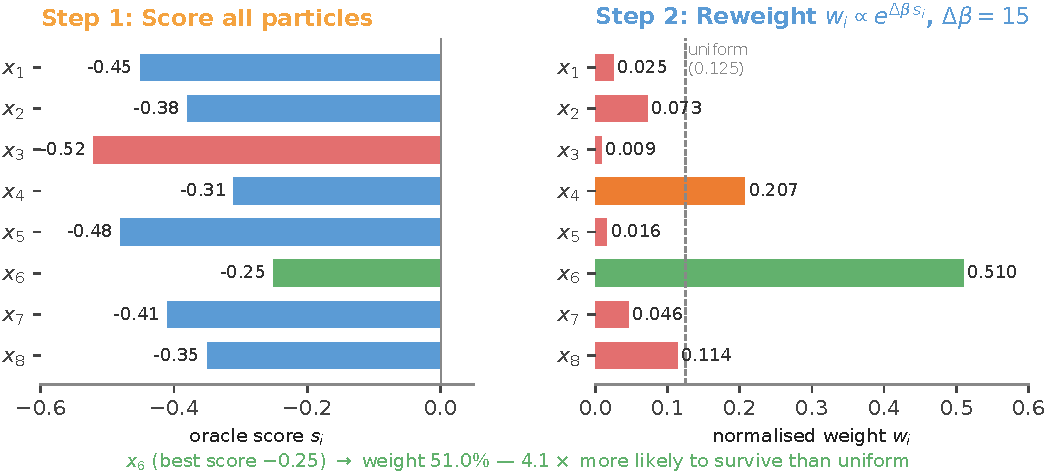
\includegraphics[width=0.95\linewidth]{figures/fig_gpa_walkthrough_score.pdf}
\caption{Score and reweight on the $N\!=\!8$ toy. \textbf{Left:} per-particle oracle scores $s_i$ (best in green: $x_6\!=\!-0.25$; worst in red: $x_3\!=\!-0.52$). \textbf{Right:} normalised weights after the tilt $w_i\!\propto\!\exp(\Delta\beta\,s_i)$ at $\Delta\beta\!=\!15$; uniform $1/N\!=\!0.125$ shown dashed. $x_6$ collects $51.0\%$ of the mass---$4.1\!\times$ the uniform expectation.}
\label{fig:walkthrough-score}
\end{figure}

\subsection{Adapting $\Delta\beta$ via bisection on $\ESS$}

The ESS-adaptive schedule (Lemma~\ref{lem:ess}) chooses $\Delta\beta_t$ so that $\ESS\!\geq\!\alpha N$ \emph{exactly} (not below). With $\alpha\!=\!0.5$, the target is $\ESS_{\rm target}\!=\!4$. Algorithm~\ref{alg:bisect} runs 64 bisection iterations on $[\Delta\beta_{\min}, \Delta\beta_{\max}]\!=\![0,1000]$.

\begin{algorithm}[h]
\caption{Bisection for $\Delta\beta$ given $\ESS$ target}\label{alg:bisect}
\begin{algorithmic}[1]
\State \textbf{Input:} scores $\{r_i\}_{i=1}^N$, target $\tau N$, range $[\Delta\beta_{\min}, \Delta\beta_{\max}]$, max iters $T_{\rm bs}$
\For{$t\!=\!1,\dots,T_{\rm bs}$}
    \State $\Delta\beta_{\rm mid}\!\leftarrow\!(\Delta\beta_{\min}+\Delta\beta_{\max})/2$
    \State $w_i\!\leftarrow\!\exp(\Delta\beta_{\rm mid}\,r_i)/Z$, with $Z\!=\!\sum_j\exp(\Delta\beta_{\rm mid}\,r_j)$
    \State $\ESS\!\leftarrow\!1/\sum_i w_i^2$
    \If{$\ESS > \tau N$} $\Delta\beta_{\min}\!\leftarrow\!\Delta\beta_{\rm mid}$ \Comment{can push harder}
    \Else \;$\Delta\beta_{\max}\!\leftarrow\!\Delta\beta_{\rm mid}$ \Comment{too aggressive}
    \EndIf
\EndFor
\State \textbf{Return:} $\Delta\beta_{\min}$
\end{algorithmic}
\end{algorithm}

For our example, the bisection converges to $\Delta\beta\!\approx\!11.7$, giving $\ESS\!\approx\!4.0\!=\!\alpha N$. The hand-picked $\Delta\beta\!=\!15$ above (which produced $\ESS\!=\!3.08$) was therefore more aggressive than the auto-schedule would choose.

\begin{figure}[h]
\centering
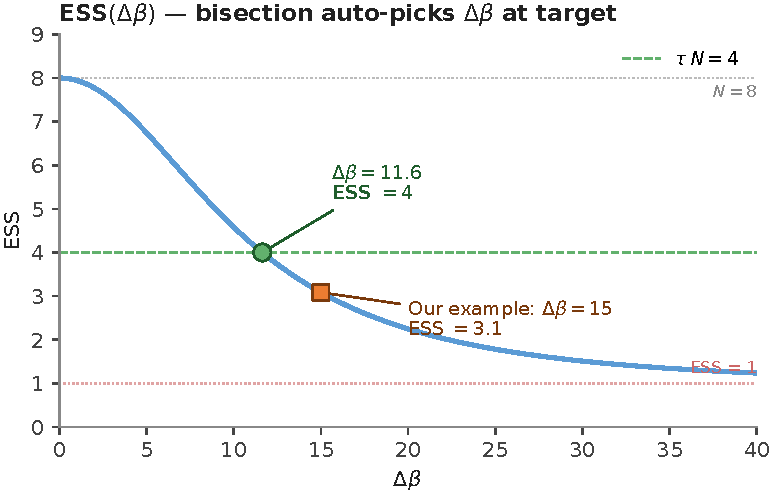
\includegraphics[width=0.78\linewidth]{figures/fig_gpa_walkthrough_ess.pdf}
\caption{$\ESS(\Delta\beta)$ for the $N\!=\!8$ toy oracle scores. The function decreases monotonically from $\ESS\!=\!N$ at $\Delta\beta\!=\!0$ toward $\ESS\!=\!1$ as $\Delta\beta\!\to\!\infty$ (winner-take-all). Bisection finds the unique $\Delta\beta\!=\!11.7$ at which $\ESS$ hits the target $\tau N\!=\!4$ (green dot). The hand-picked $\Delta\beta\!=\!15$ used in the walk-through (orange square) is past the target and so over-collapses the population.}
\label{fig:walkthrough-ess}
\end{figure}

\subsection{Resampling: multinomial vs.\ systematic}

\paragraph{Multinomial.} Draw counts $\!=\!(c_1,\dots,c_N)\!\sim\!\mathrm{Multinomial}(N, w)$. Expected copies per particle are $\E[c_i]\!=\!N\!\cdot\!w_i$, but the realised counts are noisy.

\paragraph{Systematic.} Lay the weights end-to-end as a unit interval $[0,1]$ (segment $i$ has width $w_i$). Drop $N$ pointers at positions $u\!+\!k/N$ for $k\!=\!0,\dots,N\!-\!1$, with $u\!\sim\!\mathrm{Uniform}[0,1/N)$. Particle $i$ receives a number of copies equal to the count of pointers in its segment. This has identical mean to multinomial but lower variance, and is the default in \gpa{}.

For our $N\!=\!8$ example with $u\!=\!0$, the eight pointers at $\{0.000, 0.125, 0.250, 0.375, 0.500, 0.625, 0.750, 0.875\}$ land in segments as follows: $w_2$ (cumulative 0.025--0.098) captures pointer 0.097; $w_4$ (0.107--0.314) captures pointers at 0.125, 0.250; $w_6$ (0.330--0.840) captures pointers at 0.375, 0.500, 0.625, 0.750; $w_8$ (0.886--1.000) captures pointer 0.875. Final copy counts:
\begin{center}
\begin{tabular}{lcccccccc}
\toprule
$i$       & 1 & 2 & 3 & 4 & 5 & 6 & 7 & 8 \\
copies    & 0 & 1 & 0 & 2 & 0 & 4 & 0 & 1 \\
\bottomrule
\end{tabular}
\end{center}
Four particles ($x^1, x^3, x^5, x^7$) are eliminated; $x^6$ is duplicated four times. After resampling, weights reset to $1/N\!=\!0.125$ uniformly.

\begin{figure}[h]
\centering
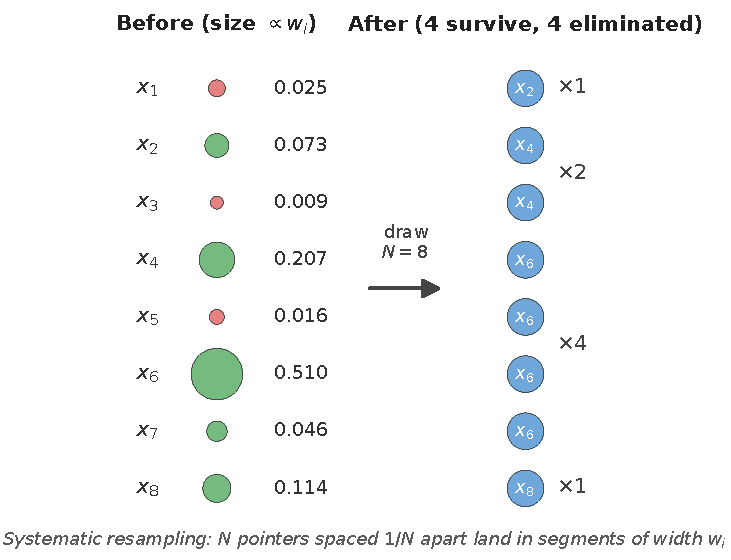
\includegraphics[width=0.85\linewidth]{figures/fig_gpa_walkthrough_resample.pdf}
\caption{Systematic resampling of the $N\!=\!8$ toy. \textbf{Left:} bubble area is proportional to $w_i$; green = retained, red = eliminated by the resampling step. \textbf{Right:} after resampling, all weights reset to $1/N$; $x_6$ now appears four times, $x_4$ twice, $x_2$ and $x_8$ once each. Four particles ($x_1, x_3, x_5, x_7$) are eliminated.}
\label{fig:walkthrough-resample}
\end{figure}

\subsection{Mutation: partial mask + denoise on a length-12 DNA toy}

Each of the eight resampled (now duplicate-rich) particles is independently mutated by $K_\beta$. Concretely, with mask fraction $\mathrm{nf}\!=\!0.25$ ($\!\to\!\lceil 0.25\!\cdot\!12\rceil\!=\!3$ positions on a length-12 sequence):
\begin{center}
\begin{tabular}{ll}
\toprule
\textbf{Step}        & \textbf{Sequence} \\
\midrule
Before (a duplicate of $x^6$)   & \texttt{ACGTATGCACGT} \\
Random mask 3 positions          & \texttt{AC?TA?GC?CGT} \\
Denoise via $p_\theta$           & \texttt{AC\textbf{T}TA\textbf{A}GC\textbf{A}CGT} \\
\midrule
Net edits                         & pos 3: G$\to$T; \, pos 6: T$\to$A; \, pos 9: C$\to$A \\
\bottomrule
\end{tabular}
\end{center}
Two properties this kernel inherits from the pretrained $p_\theta$:
\begin{itemize}
\item \emph{Grammar preservation.} The denoiser sees the unmasked context and proposes tokens consistent with whatever motif/composition rules $p_\theta$ has learned. Random per-position resampling would not.
\item \emph{Diversity restoration.} The four duplicates of $x^6$ each get an \emph{independent} random mask + denoising pass, so they diverge into four distinct child sequences. Without mutation the population would collapse to four identical copies.
\end{itemize}
The mask fraction $\mathrm{nf}$ controls exploration: $\mathrm{nf}\!=\!0.05$ is local search ($\sim\!10$ positions per step on a 200-bp DNA enhancer), $\mathrm{nf}\!=\!0.20$ is large jumps. Section~\ref{sec:results:ablation} reports sensitivity in the practical range.

%-----------------------------------------------------------------------
\section{Hyperparameters}\label{app:hyper}

Table~\ref{tab:hyper-rerd} lists hyperparameters for the SMC-protocol comparison (\drakes{} eval pair); Table~\ref{tab:hyper-ctrldna} lists those for \ctrldna{} comparison (HyenaDNA + gReLU MSE oracles); Table~\ref{tab:hyper-dnacraft} for \dnacraft{} comparison (HyenaDNA/DiMamba + Enformer 50/50). Default values are bolded.

\begin{table}[h]
\caption{Hyperparameters for the SMC-protocol comparison (HepG2 enhancer, MDLM backbone, \drakes{} split-oracle).}
\label{tab:hyper-rerd}
\centering
\small
\begin{tabular}{lll}
\toprule
Parameter & Mean recipe & Spec recipe \\
\midrule
$N$ (population) & 5000 & 5000 \\
$\alpha$ (ESS threshold) & 0.5 & 0.5 \\
$\beta_*$ (target inverse temp) & 200 & 100 \\
$T_{\max}$ (max steps) & 30, hard cap 200 & 30, hard cap 200 \\
nf (mask fraction) & 0.05 & 0.05 \\
DPS gradient strength $\eta$ & 3000 & 3000 \\
$\mathrm{pw}$ (off-target penalty) & 0 & 0.35 \\
GC bio-filter & [0.45, 0.55] & [0.45, 0.55] \\
\bottomrule
\end{tabular}
\end{table}

\begin{table}[h]
\caption{Hyperparameters for \ctrldna{} comparison (Reddy promoters, HyenaDNA backbone, gReLU MSE oracles, universal recipe).}
\label{tab:hyper-ctrldna}
\centering
\small
\begin{tabular}{ll}
\toprule
Parameter & Universal recipe \\
\midrule
$N$ (population) & 10000 \\
$\alpha$ (ESS threshold) & 0.5 \\
$\beta_*$ & 100 \\
$T_{\max}$ (steps) & 60 \\
nf (mask fraction) & 0.05 \\
$K$ (branch factor) & 8 \\
$\mathrm{pw}$ & 0.35 \\
diversity $\lambda$ (conformity) & \textbf{1.0} \\
DPS & off \\
GC bio-filter & off \\
\bottomrule
\end{tabular}
\end{table}

\begin{table}[h]
\caption{Hyperparameters for \dnacraft{} comparison (Gosai 50/50 split, top-128 by MinGap-Eval). C1 = no GC penalty; C3 = soft GC penalty (gct=0.60), no hard bio-filter.}
\label{tab:hyper-dnacraft}
\centering
\small
\begin{tabular}{lll}
\toprule
Parameter & C1 & C3 \\
\midrule
$N$ (population) & 5000 & 5000 \\
$\beta_*$ & 25 & 25 \\
$\mathrm{pw}$ & 0.30 & 0.30 \\
DPS & on & on \\
GC penalty (gct) & --- & 0.60 \\
GC bio-filter & off & off \\
$K$ & 8 & 8 \\
\bottomrule
\end{tabular}
\end{table}

%-----------------------------------------------------------------------
\section{Full GPA-vs-ISM/LEDIDI tables}\label{app:ism_full}

Single-sequence comparison: GPA row = the one sequence in each pool that maximises $\mathrm{AG}-\mathrm{LN}$ (sweet spot: low LN, high held-out AG). Directly comparable to \ism{}/\ledidi{} which are inherently single-sequence.

\begin{table}[h]
\caption{Single-sequence comparison, K562 enhancer, two seeds (uid=181692 natural, uid=50178 random). \gpa{} row = argmax of $\mathrm{AG}-\mathrm{LN}$ within the 5{,}000-seq pool.}
\label{tab:ism_singleseq}
\centering
\small
\begin{tabular}{llrrr}
\toprule
Seed & Method & Edits & LN & AG \\
\midrule
\multirow{4}{*}{uid=181692}
 & \gpa{} (no DPS) uncap   &  96 & 4.97 & \textbf{3.33} \\
 & \gpa{} (+DPS) cap30     &  60 & 6.21 & \textbf{3.47} \\
 & \ism{} gen 115          & 115 & 8.74 & 2.83 \\
 & \ledidi{} t15 $\lambda$=0.05 & 125 & 9.81 & $-$0.22 \\
\midrule
\multirow{4}{*}{uid=50178}
 & \gpa{} (no DPS) cap30   &  60 & 4.71 & 2.75 \\
 & \gpa{} (+DPS) cap30     &  59 & 6.58 & \textbf{3.61} \\
 & \ism{} gen 115          & 115 & 9.58 & 2.92 \\
 & \ledidi{} t15 $\lambda$=0.05 & 105 &11.66 & $-$0.62 \\
\bottomrule
\end{tabular}
\end{table}

\paragraph{Reading the table.}
A single \gpa{} sequence (e.g.\ +DPS cap30 on uid=50178: LN $6.58$, AG $3.61$) beats \ism{} gen 115 on the held-out AG by $+0.69$ at LN $\sim\!3.0$ lower—better held-out activity \emph{and} less reward-hacking. Under any selection rule, \ledidi{} stays AG-negative; not one of its 50 reruns produces an AG-positive sequence.

\paragraph{Apples-to-apples runtime (single H100, K562 enhancer, 5{,}000-sequence pool).}
Table~\ref{tab:ism_runtime} reports wall-time at matched output volume, averaged across the random and natural pools. \gpa{} is fully population-parallel: a single SMC step propagates all 5{,}000 particles together through the diffusion proposal, so the per-particle cost is the GPU-memory chunk \texttt{mutation\_batch\_size=128} amortised over the population. \ism{} is also nominally population-parallel (5{,}000 independent greedy trajectories), but its sequential cost is fixed at 115 generations per seed, and that dominates wall regardless of how memory chunks are batched. \ledidi{} is chunked-sequential by design: 5{,}000 seeds processed in 39 chunks of 128 along the Gumbel-softmax optimisation. The result is $\sim\!9.3\times$ speedup over \ism{} and $\sim\!3.4\times$ speedup over \ledidi{} at identical pool size and identical hardware.

\begin{table}[h]
\caption{Apples-to-apples runtime: single H100, 5{,}000-sequence K562-enhancer pool, averaged across random and natural seed pools. \gpa{} = v3 noDPS recipe (matches Sec.~\ref{sec:results:ism}). Speedup column is $\mathrm{wall}_{\text{baseline}}/\mathrm{wall}_{\gpa{}}$.}
\label{tab:ism_runtime}
\centering
\small
\begin{tabular}{lllr}
\toprule
Method & Wall (5K pool) & Parallelism & Speedup vs.\ \gpa{} \\
\midrule
\textbf{\gpa{}} & \textbf{$\sim\!11.6$ min} & population-parallel (5{,}000 SMC particles) & --- \\
\ledidi{}       & $\sim\!40$ min     & chunked-sequential (39 chunks $\times$ 128 seeds) & $\sim\!3.4\times$ slower \\
\ism{}          & $\sim\!107.5$ min  & population-parallel, but 115 sequential greedy gens & $\sim\!9.3\times$ slower \\
\bottomrule
\end{tabular}
\end{table}

%-----------------------------------------------------------------------
\section{Full DNA-CRAFT tables (GPA-C1 vs GPA-C3)}\label{app:dnacraft_full}

The headline column in Table~\ref{tab:dnacraft} uses GPA-C3 (\texttt{dps\_pw030\_b25\_gct060\_nobio}). This appendix shows the same benchmark with the alternate recipe variant GPA-C1 (\texttt{dps\_pw030\_b25}, no GC penalty), under the matched-output-budget protocol of Table~\ref{tab:dnacraft} (\texttt{by\_pool\_composite} top-64 from \texttt{gpa\_output\_best\_eval.h5}, 3 reps for both variants). Both variants run at $\sim\!3.6$ min/seed (no MCTS) on the MDLM backbone; the only difference is the soft GC-centering term added to C3's DPS gradient.

\paragraph{Recipe decomposition.}
Each token in the recipe name maps to a specific knob in the GPA algorithm of \S\ref{sec:method}, with no other differences between the two variants:
\begin{itemize}
\item \texttt{dps} -- enables the Gumbel-softmax oracle gradient with strength $\eta\!=\!3000$ (\S\ref{sec:method:ext}, ``Gumbel-softmax oracle gradient (DPS)''). This is a biased proposal in the sense of \S\ref{sec:method:ext} and is shared by both C1 and C3, so the C1$\leftrightarrow$C3 contrast does not move along the DPS-bias axis.
\item \texttt{pw030} -- sets the off-target weight $\mathrm{pw}\!=\!0.30$ in the linear fitness of Eq.~\ref{eq:fitness} (\S\ref{sec:method:pw}); the same $0.30$ weights the off-target term inside the DPS gradient as well.
\item \texttt{b25} -- sets the SMC tilt ceiling $\beta_*\!=\!25$. This is below the default range $\beta_*\!\in\!\{100,200\}$ in \S\ref{sec:exp} and is a deliberately gentler tilt that preserves population diversity at some cost in MinGap; both variants share it.
\item \texttt{gct060} \emph{(C3 only)} -- adds a quadratic centering term $-w\,(g(x)-0.60)^2$ to the DPS objective before backpropagation, where $g(x)\!=\!\overline{P(C)+P(G)}$ is the per-position soft-onehot GC fraction and $w\!=\!10$. The penalty rides inside the same Gumbel-softmax gradient that DPS already computes; it is \emph{not} a hard accept/reject filter.
\item \texttt{nobio} -- disables the hard bio-filter (no \texttt{gc\_low}/\texttt{gc\_high} interval gating). All GC discipline in C3 therefore comes from the soft \texttt{gct060} term in the DPS gradient.
\end{itemize}
Both variants additionally use the default branch factor $K\!=\!8$ (\S\ref{sec:method:ext}, Prop.~\ref{prop:K}) and population $N\!=\!5{,}000$ (Table~\ref{tab:dnacraft} caption), so both target $\pi_{\beta_*}^{(K=8)}\!\neq\!\pi_{\beta_*}$ in the sense of Prop.~\ref{prop:K}; the C1$\leftrightarrow$C3 contrast isolates the GC-centering term with $K$, $\beta_*$, $\mathrm{pw}$, $N$, and the DPS bias all held constant.

\begin{table}[h]
\caption{\dnacraft{} benchmark with the GPA-C1 alternate recipe (\texttt{dps\_pw030\_b25}; no GC penalty), reported alongside the headline GPA-C3 (Table~\ref{tab:dnacraft}). Both columns: \texttt{by\_pool\_composite} top-64 from \texttt{gpa\_output\_best\_eval.h5}, mean (std) over 3 reps. Baselines verbatim from \citet{dnacraft2026}.}
\label{tab:dnacraft_full_eval}
\centering
\scriptsize
\begin{tabular}{llcccccccccc}
\toprule
Cell & Metric & SMC & CG & TDS & DRAKES & D3 & Ledidi & Ctrl-DNA & DNA-CRAFT & \gpa{}-C1 & \gpa{}-C3 \\
\midrule
\multirow{4}{*}{HepG2}
 & MinGap   & 1.61 & $-$0.23 & 0.40 & $-$1.40 & 0.05 & 5.77 & \textbf{7.79} & 4.35 & 6.87 & 6.91 \\
 & Motif    & 0.55 & 0.86 & 0.40 & 0.06 & 0.87 & 0.58 & 0.63 & \textbf{0.92} & 0.90 & \textbf{0.92} \\
 & 3-mer    & 0.81 & 0.97 & 0.74 & $-$0.36 & \textbf{0.98} & 0.76 & 0.49 & \textbf{0.98} & 0.95 & 0.95 \\
 & Diversity& 0.83 & \textbf{1.98} & 0.96 & 1.86 & \textbf{1.98} & \textbf{1.98} & 1.90 & \textbf{1.98} & 1.81 & 1.86 \\
\midrule
\multirow{4}{*}{K562}
 & MinGap   & 4.12 & 0.00 & 1.62 & $-$0.20 & 0.18 & 7.66 & \textbf{9.07} & 5.69 & 8.18 & 8.13 \\
 & Motif    & 0.45 & 0.85 & 0.51 & 0.14 & 0.86 & 0.65 & 0.63 & 0.93 & 0.93 & \textbf{0.94} \\
 & 3-mer    & 0.66 & 0.94 & 0.65 & $-$0.35 & 0.96 & 0.69 & 0.41 & \textbf{0.98} & 0.92 & 0.95 \\
 & Diversity& 0.31 & \textbf{1.98} & 0.64 & 1.96 & \textbf{1.98} & \textbf{1.98} & 1.90 & \textbf{1.98} & 1.56 & 1.83 \\
\midrule
\multirow{4}{*}{SK-N-SH}
 & MinGap   & 0.56 & $-$0.28 & 0.19 & 0.09 & $-$0.01 & 3.03 & 3.72 & 3.23 & \textbf{5.07} & 4.98 \\
 & Motif    & 0.52 & 0.86 & 0.48 & 0.23 & 0.84 & 0.38 & 0.48 & 0.88 & 0.89 & \textbf{0.92} \\
 & 3-mer    & 0.78 & 0.95 & 0.72 & $-$0.38 & 0.93 & 0.37 & 0.20 & \textbf{0.97} & 0.87 & 0.94 \\
 & Diversity& 1.27 & \textbf{1.98} & 0.92 & 1.83 & 1.97 & \textbf{1.98} & 1.86 & \textbf{1.98} & 1.59 & 1.86 \\
\bottomrule
\end{tabular}
\end{table}

\paragraph{Reading.}
GPA-C1 and GPA-C3 give nearly tied MinGap and Motif Spearman on every cell (within seed std on most rows). C3 wins Motif on HepG2 / K562 / SK-N-SH ($+0.02$/$+0.01$/$+0.03$) and 3-mer on K562 / SK-N-SH ($+0.03$/$+0.07$). The biggest practical difference is Diversity: the soft GC-centering term in C3's DPS gradient recovers $+0.05$ to $+0.27$ Shannon bits over C1 on every cell, lifting C3 above the Ctrl-DNA Diversity floor on all three cells. The mechanism is indirect: by penalising drift away from $g(x)\!=\!0.60$ at every Gumbel-softmax step, the term blunts the oracle's tendency to push particles toward narrow high-GC modes, which in turn keeps the population spread out in sequence space. C1 wins MinGap on K562 / SK-N-SH ($+0.05$/$+0.09$) but loses across the rest. C3 is the headline because the +Diversity / +Motif / +3-mer trade dominates the small MinGap give-back; C1 is reported as an ablation that isolates the GC-penalty's contribution.

\paragraph{Backbone caveat.}
\dnacraft{}'s reported numbers in Table~\ref{tab:dnacraft} are obtained on a Mamba-style discrete-diffusion (DiMamba) backbone whose code and pretrained checkpoints are not publicly available; the same paper also reports DiMamba-vs-MDLM ablations that show DiMamba contributes additional biological-faithfulness gains. Our \gpa{}-C1 / \gpa{}-C3 numbers are obtained on the publicly available MDLM backbone of \citet{sahoo2024mdlm} and should be read as a lower bound on what \gpa{} would achieve at backbone parity, by Remark~\ref{rem:agnostic}.

%-----------------------------------------------------------------------
\section{Wall-time table}\label{app:wall}

\begin{table}[h]
\caption{Wall time per seed and 5-seed totals (HepG2, identical H100 hardware, identical HyenaDNA backbone). Wall time excludes downstream motif scoring.}
\label{tab:wall}
\centering
\small
\begin{tabular}{lrr}
\toprule
Method & Wall/seed (h) & 5-seed total (GPU-h) \\
\midrule
\ctrldna{} R200 (RL fine-tune) & $43.5\pm 0.8$ & $\sim\!218$ \\
\gpa{} v3 (K=8, no diversity)  & $3.97\pm 0.59$ & 19.8 \\
\gpa{} v4 (K=8 + rejuvenation) & $2.17\pm 0.22$ & 10.8 \\
\gpa{} v5 (K=8 + diversity)    & $\mathbf{2.22\pm 0.52}$ & $\mathbf{11.1}$ \\
\bottomrule
\end{tabular}
\end{table}

%-----------------------------------------------------------------------
\section{DPS gradient ablation}\label{app:dps_ablation}

Population annealing alone (no DPS) already beats single-chain refinement baselines; DPS gradient is a multiplicative enhancement.

\begin{table}[h]
\caption{DPS gradient ablation on Gosai HepG2.}
\label{tab:dps_ablation}
\centering
\small
\begin{tabular}{llrrr}
\toprule
Track & Metric & \gpa{}-only & \gpa{}+DPS & $\Delta$(DPS) \\
\midrule
Mean & $H_{\mathrm{eval}}$ & $8.73\pm 0.50$ & $\mathbf{10.06\pm 0.19}$ & $+1.33$ \\
Mean & Spec & 1.58 & 3.06 & $+1.48$ \\
Spec & $H_{\mathrm{eval}}$ & $8.28\pm 0.12$ & $9.35\pm 0.20$ & $+1.07$ \\
Spec & Spec & $6.11\pm 1.45$ & $\mathbf{7.61\pm 0.25}$ & $+1.50$ \\
\bottomrule
\end{tabular}
\end{table}

%-----------------------------------------------------------------------
\section{Naturalness audit}\label{app:naturalness}

\begin{table}[h]
\caption{Naturalness audit (HepG2 top-128). \gpa{} produces bio-plausible sequences by construction; \ctrldna{} reward-hacks to non-biological space.}
\label{tab:nat}
\centering
\small
\begin{tabular}{lrrr}
\toprule
Metric & Real (Gosai) & \gpa{} & \ctrldna{} \\
\midrule
GC mean & 0.44 & 0.41 & 0.45 \\
\textbf{bio\_pass\_rate} & 0.51 & $\mathbf{1.00}$ & $\mathbf{0.05}$ \\
max homopolymer & 5.4 & 5.1 & $\mathbf{20.9}$ \\
$k$=3 Pearson & 1.0 & 0.61 & 0.39 \\
HNF1A enrichment & $0\times$ & $10\,040\times$ & $7\,812\times$ \\
\bottomrule
\end{tabular}
\end{table}

\begin{figure}[h]
\centering
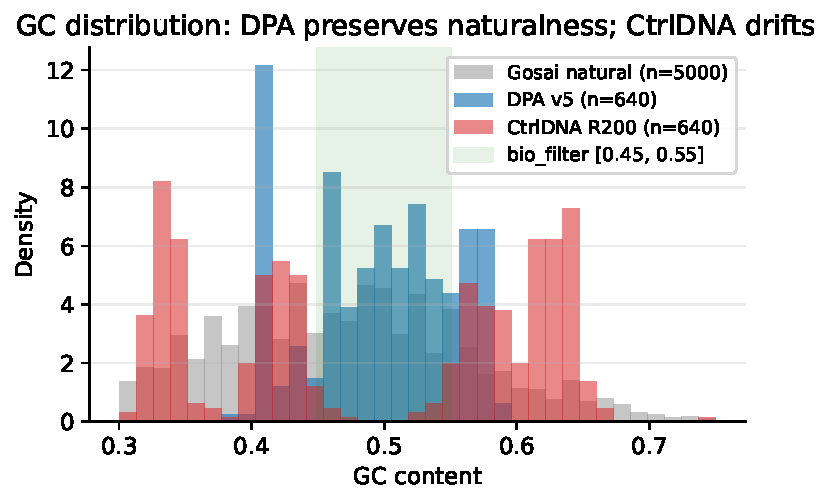
\includegraphics[width=0.6\linewidth]{figures/fig2_gc.pdf}
\caption{GC distribution comparison on HepG2 top-128 sequences. \gpa{} (blue) clusters near the lower edge of the bio-filter (45\%) but stays within the natural Gosai range (gray); \ctrldna{} (red) drifts widely, with a heavy tail of low- and high-GC sequences and a substantial fraction outside the natural distribution.}
\label{fig:gc}
\end{figure}

%-----------------------------------------------------------------------
\section{Extreme specificity}\label{app:extreme}

Pushing $\mathrm{pw}$ beyond the canonical $0.35$ trades $H_{\mathrm{eval}}$ for higher specificity until both off-targets fall below baseline (Table~\ref{tab:extreme}).

\begin{table}[h]
\caption{Extreme-specificity extension on Gosai HepG2 (single run each, $N\!=\!5000$).}
\label{tab:extreme}
\centering
\small
\begin{tabular}{rrrrr}
\toprule
$\mathrm{pw}$ & $H_{\mathrm{eval}}$ & $K_{\mathrm{eval}}$ & $S_{\mathrm{eval}}$ & $H{>}8 \wedge K{<}0 \wedge S{<}0$ \\
\midrule
0.35 & 9.65 & 2.15 &  1.10 & 0 \\
0.50 & 9.54 & 1.96 &  0.63 & 0 \\
0.70 & 8.73 & 1.52 &  0.35 & 0 \\
1.00 & 8.57 & 0.69 & $-$0.48 & 26 \\
1.50 & $\mathbf{8.44}$ & 0.55 & $\mathbf{-0.66}$ & $\mathbf{54}$ \\
\bottomrule
\end{tabular}
\end{table}

\paragraph{Beta trajectory.}
Figure~\ref{fig:beta} shows a representative ESS-adaptive $\beta$ trajectory and the population-mean reward over SMC steps for a HepG2 run.

\begin{figure}[h]
\centering
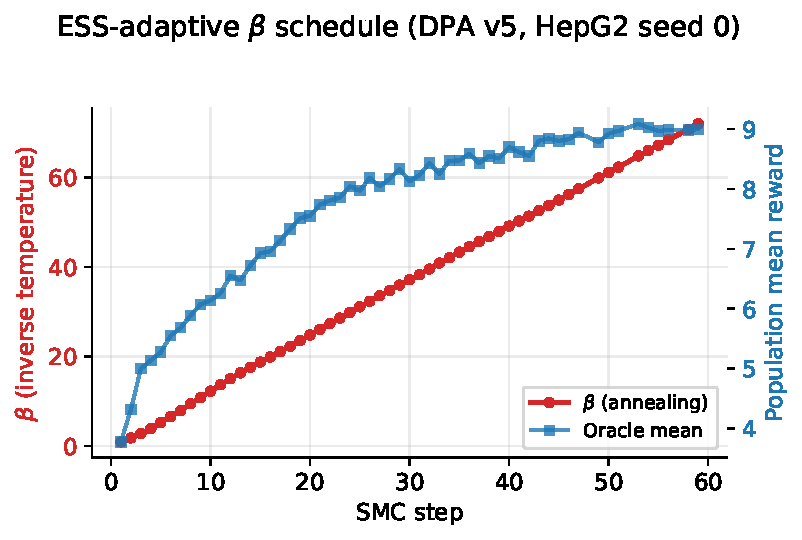
\includegraphics[width=0.6\linewidth]{figures/fig4_beta_traj.pdf}
\caption{Representative \gpa{} run trajectory (HepG2, seed 0). Red trace: ESS-adaptive $\beta$ schedule rises through the annealing path. Blue trace: population mean reward grows monotonically toward saturation as $\beta$ increases.}
\label{fig:beta}
\end{figure}

%-----------------------------------------------------------------------
\section{Negative result: APF correction for $\epsilon$-greedy $K$-branching}\label{app:apf}

A natural attempt to recover Shannon under $K$-branching is to soften the argmax with $\epsilon$-greedy ($\tau\!>\!0$ softmax over the $K$ siblings) and apply the auxiliary-particle-filter weight correction \citep{pittshephard1999}:
\[
w_{\mathrm{new}} = w_{\mathrm{old}}\big/p_\tau(\mathrm{winner}),\qquad p_\tau(j)=\exp(r_j/\tau)\big/\sum_m\exp(r_m/\tau).
\]
Compute the expectation:
\[
\E[w_{\mathrm{new}}\,\varphi(x_{\mathrm{winner}})] = \E_{x_{1:K}\sim q}\!\!\left[\sum_{j=1}^K \frac{\exp(r_j/\tau)}{\sum_m\exp(r_m/\tau)}\cdot\frac{\sum_m\exp(r_m/\tau)}{K\exp(r_j/\tau)}\,\varphi(x_j)\right]=\frac{1}{K}\sum_j \E_q[\varphi(x_j)],
\]
i.e.\ the corrected estimator is equivalent to a single-child sample. The $K$ siblings collapse and the effective-$\beta$ boost vanishes. Empirically, on a synthetic linear reward $r(x)\!=\!3x$ with $q$ uniform on $[0,1]$ (200K Monte-Carlo trials):
\begin{center}
\small
\begin{tabular}{lrrr}
\toprule
Variant & $\E[x]$ & $\mathrm{Var}[x]$ & ESS \\
\midrule
$K=1$ no selection                & 0.5000 & 0.0833 & 100.0\% \\
$K=8$ argmax (no correction)      & 0.8887 & 0.0099 & 100.0\% \\
$K=8$ softmax $\tau\!=\!0.3$ (no corr.) & 0.8445 & 0.0180 & 100.0\% \\
\textbf{$K=8$ softmax $\tau\!=\!0.3$ + APF} & 0.4880 & 0.0874 & 0.4\% \\
$K=8$ softmax $\tau\!=\!1.0$ + APF & 0.5009 & 0.0829 & 53.1\% \\
\bottomrule
\end{tabular}
\end{center}
ESS collapses at low $\tau$ and the corrected mean/variance reproduces $K=1$. We therefore do \emph{not} use APF correction for production runs and report only argmax $K$-branching. K-annealing schedules and waste-free SMC \citep{dau2022wastefree} remain valid theoretical alternatives, deferred to future work.

%-----------------------------------------------------------------------
\section{Negative result: post-hoc Metropolis tempering}\label{app:posthoc}

Another natural Shannon-rescue move is to load the concentrated argmax-$K$ pool and run Metropolis–Hastings at lower $\beta'$ to spread the population. We tested this on the K562 promoter pool (50 MH steps, nf=0.05, HyenaDNA proposal):

\begin{center}
\small
\begin{tabular}{rrrrr}
\toprule
$\beta'$ & accept rate & $\Delta$comp & $\Delta$tgt & $\Delta H$ \\
\midrule
25 &  3.4\% & $+0.02$ & $-0.06$ & $+0.05$ \\
12 &  6.5\% & $-0.15$ & $-0.27$ & $+0.10$ \\
 6 & 13.1\% & $-0.68$ & $-0.77$ & $+0.21$ \\
 3 & 29.1\% & $-2.12$ & $-2.22$ & $+0.39$ \\
 1 & 73.7\% & $-4.71$ & $-5.35$ & $+0.61$ \\
\bottomrule
\end{tabular}
\end{center}
The Pareto slope is $\sim\!3\!-\!5$ target units per $0.1$ nat of Shannon, far too steep for the diversity gap to \dnacraft{}/\ctrldna{} K562 ($\sim\!0.5$ nat) to be closed without erasing the target advantage. Increasing chain length or shrinking nf does not change the local-neighborhood geometry. The honest reading: under sharply peaked oracles, the activity–diversity tension is in the reward landscape, not the sampler.

%-----------------------------------------------------------------------
\section{GC distribution and floor-hugging}\label{app:gc}

Even with the bio-filter $\mathrm{GC}\!\in\![0.45,0.55]$, $60\!-\!75\%$ of \gpa{} top-128 sequences cluster at the lower bound. Two facts:
\begin{enumerate}
\item This is a property of the \emph{masked-diffusion proposal} at low noise fraction. At $\mathrm{nf}\!=\!0.20$ the bias inverts toward the upper bound (GC $\approx\!0.54$); the crossover occurs near $\mathrm{nf}\!\approx\!0.16\!-\!0.17$.
\item The eval oracle is GC-agnostic: at both $\mathrm{nf}$ extremes, top-128 oracle scores are comparable. The GC bias arises from $p_\theta$, not from the reward signal.
\end{enumerate}
Three mitigations were tested with mixed success: (i) GC-aware DPS gradient (\verb|gc_dps_weight|) reduces floor-hugging from $61.5\%$ to $55.0\%$ at $-0.09$ $H_{\mathrm{eval}}$ cost; (ii) narrow $1\%$ GC bands achieve uniform GC by construction at $-0.25$ $H_{\mathrm{eval}}$; (iii) stratified resampling within $2\%$ GC bins \citep{verge2015island} achieves balanced coverage at $-0.50$ to $-1.0$ $H_{\mathrm{eval}}$. We report all three options in the codebase but use the unmitigated baseline in the headline tables for fair comparison with peer methods.

%-----------------------------------------------------------------------
\section{Ctrl-DNA enhancer comparison (V7 main + V5/V8 ablations)}\label{app:ctrldna_enhancer}

This appendix gives the dedicated \ctrldna{}-vs-\gpa{} enhancer comparison referenced in \S\ref{sec:results:promoter}. Same Gosai 50/50 split as the \dnacraft{} benchmark, top-128 selection per cell, 5 \gpa{} seeds. The headline GPA recipe is V7 (universal: $K\!=\!8$, diversity $\lambda\!=\!1.0$); V8a, V8b (alternative pairwise-suppression formulations) and V5 (the previous default with $\lambda\!=\!0.2$) are ablations.

\begin{table}[h]
\caption{Ctrl-DNA vs.\ \gpa{} on Gosai HepG2/K562/SKNSH enhancers (5 seeds; mean (std)). Headline = V7 universal recipe; V8a (log\_ratio + pw=1.0), V8b (linear + pw=1.0) and V5 ($\lambda\!=\!0.2$) are ablations of the diversity / pairwise-suppression knob. \texttt{target\_raw} = mean target oracle score; \texttt{ΔR} = normalised target minus mean off-target; \texttt{shannon} = per-position entropy; \texttt{motif\_corr} = FIMO Pearson against per-cell real reference.}
\label{tab:ctrldna_enhancer}
\centering
\footnotesize
\setlength{\tabcolsep}{4pt}
\begin{tabular}{llrrrr}
\toprule
Cell & Method & target\_raw $\uparrow$ & ΔR $\uparrow$ & shannon $\uparrow$ & motif\_corr $\uparrow$ \\
\midrule
\multirow{5}{*}{HepG2}
 & \ctrldna{} R200             & 5.32 (0.65) & 0.48 (0.10) & 1.65 (0.14) & \textbf{0.29} (0.16) \\
 & \gpa{} V5 ($K\!=\!8, \lambda\!=\!0.2$) & 9.86 (0.10) & 0.85 (0.01) & 1.49 (0.03) & 0.19 (0.03) \\
 & \gpa{} V7 ($K\!=\!8, \lambda\!=\!1.0$) & \textbf{9.90} (0.12) & 0.84 (0.02) & 1.59 (0.11) & 0.20 (0.02) \\
 & \gpa{} V8a (log\_ratio, pw=1.0) & 6.61 (0.04) & 0.68 (0.01) & \textbf{1.93} (0.00) & 0.15 (0.02) \\
 & \gpa{} V8b (linear, pw=1.0) & 9.51 (0.10) & \textbf{0.93} (0.02) & 1.70 (0.11) & 0.10 (0.04) \\
\midrule
\multirow{5}{*}{K562}
 & \ctrldna{} R200             & \textbf{9.99} (1.52) & \textbf{0.77} (0.14) & 1.60 (0.15) & 0.24 (0.07) \\
 & \gpa{} V5 ($K\!=\!8, \lambda\!=\!0.2$) & 8.82 (0.13) & 0.34 (0.00) & 1.43 (0.09) & \textbf{0.26} (0.02) \\
 & \gpa{} V7 ($K\!=\!8, \lambda\!=\!1.0$) & 8.83 (0.12) & 0.32 (0.01) & 1.65 (0.02) & 0.24 (0.02) \\
 & \gpa{} V8a (log\_ratio, pw=1.0) & 6.48 (0.03) & 0.39 (0.01) & \textbf{1.94} (0.01) & 0.24 (0.01) \\
 & \gpa{} V8b (linear, pw=1.0) & 8.15 (0.04) & 0.41 (0.01) & 1.68 (0.02) & 0.25 (0.02) \\
\midrule
\multirow{5}{*}{SK-N-SH}
 & \ctrldna{} R200             & 9.93 (1.13) & \textbf{0.71} (0.10) & 1.63 (0.17) & \textbf{0.23} (0.10) \\
 & \gpa{} V5 ($K\!=\!8, \lambda\!=\!0.2$) & \textbf{14.33} (0.20) & 0.10 (0.01) & 1.49 (0.04) & \textbf{0.23} (0.01) \\
 & \gpa{} V7 ($K\!=\!8, \lambda\!=\!1.0$) & 14.17 (0.18) & 0.10 (0.00) & 1.63 (0.04) & 0.20 (0.01) \\
 & \gpa{} V8a (log\_ratio, pw=1.0) & 6.29 (0.08) & 0.22 (0.01) & \textbf{1.91} (0.01) & 0.15 (0.01) \\
 & \gpa{} V8b (linear, pw=1.0) & 8.26 (0.15) & 0.29 (0.03) & 1.74 (0.05) & 0.10 (0.01) \\
\bottomrule
\end{tabular}
\end{table}

\paragraph{Headlines.}
\gpa{} V7 (the universal recipe) wins target\_raw on HepG2 and SK-N-SH ($+4.58$ and $+4.24$ over \ctrldna{}), and is competitive on K562 within $\sim$1 std. \ctrldna{} retains a ΔR (specificity) edge on K562 and SK-N-SH at the cost of $\sim$50\% lower target activity on HepG2/SK-N-SH and high seed-to-seed variance ($\pm 1.13$--$1.52$). The V7 vs.\ V5 comparison shows the diversity-$\lambda$ bump (from $0.2$ to $1.0$) buys $+0.10$--$0.22$ shannon on every cell at zero target cost, isolating the population-conformity penalty as a strict Pareto improvement. V8a/V8b are alternative pairwise-suppression formulations: V8a (log-ratio reward, pw=1.0) achieves the tightest shannon ($1.91$--$1.94$, near uniform) but at substantial target cost; V8b (linear, pw=1.0) recovers HepG2/K562 target while maximising HepG2 ΔR. The four GPA variants together trace a Pareto front in (target, shannon, motif) space at fixed inference cost---one knob per recipe, no retraining.

%-----------------------------------------------------------------------
\section{DNA-CRAFT $K$ and $i$ scaling sweeps (UCB-MCTS variant)}\label{app:ucb_scaling}

\paragraph{Why MCTS at all.}
DNA-CRAFT replaces the SMC population with a single depth-bounded Monte Carlo Tree Search loop on a DiMamba diffusion backbone, and shows that this delivers state-of-the-art motif and 3-mer grammar fidelity on the Gosai enhancer benchmark (Table~\ref{tab:dnacraft}). The mechanism that delivers their grammar bar is plausible on its face: tree search amortises the cost of choosing the right next mutation by replaying the same scoring oracle across multiple competing children before committing—a strictly more informed proposal than picking the first child that scores well. \gpa{}'s standard $K$-branch is a depth-1 special case of this idea: try $K$ candidates from the proposal and keep the best (Sec.~\ref{sec:method:ext}). It is natural to ask whether the same \emph{deeper} planning that powers \dnacraft{}'s grammar—expanding the best leaves over multiple iterations rather than just one---closes \gpa{}'s residual gap to \dnacraft{} on motif/3-mer correlation. The \texttt{ucb\_stacked} variant exists to test exactly that question.

\paragraph{What \texttt{ucb\_stacked} does, step by step.}
At every SMC mutation step, each particle $x_t^{(j)}$ becomes the root of an independent Monte Carlo tree. We then run $i$ iterations on that tree, where each iteration follows the standard four-phase MCTS-with-UCB1 loop \citep[``UCT'';][]{kocsis2006uct}:
\begin{enumerate}
\item \emph{Selection.} Traverse from the root to a leaf by greedily picking, at each internal node $v$ with already-expanded children $\{a\}$, the child that maximises the UCB1 score \citep{auer2002ucb,kocsis2006uct}
\begin{equation}\label{eq:ucb1}
    \mathrm{UCB1}(a) \;=\; \bar{Q}(a) \;+\; c\sqrt{\frac{\ln n(v)}{n(a)}},
\end{equation}
where $\bar{Q}(a)\!\in\![0,1]$ is the mean (range-normalised) reward backed up through child $a$, $n(a)$ is the visit count of $a$, $n(v)\!=\!\sum_a n(a)$ is the parent visit count, and $c\!=\!\sqrt{2}$ is the standard exploration constant. The first term exploits children with high empirical value; the second term explores low-visit children with a $\sqrt{\log n / n(a)}$ confidence radius. Together this is the canonical bandit rule of \citet{auer2002ucb} for stochastic multi-armed bandits, and \citet{kocsis2006uct} show that applying it node-wise inside a tree (UCT) inherits the same $\mathcal{O}(\log n)$ regret bound at each node. Children with $n(a)\!=\!0$ are tried first by convention so the second term remains well-defined.
\item \emph{Expansion.} Apply \gpa{}'s standard $K$-branch operator at the selected leaf: draw $K\!=\!8$ children using partial-mask$\circ$denoise + DPS (the same operator the no-MCTS \gpa{} would use as its mutation kernel).
\item \emph{Evaluation.} Score each new child under the eval-side reward.
\item \emph{Backpropagation.} Update visit counts $n(\cdot)$ and value estimates $\bar{Q}(\cdot)$ along the path from each new child up to the root, so the next iteration's UCB1 selection (Eq.~\ref{eq:ucb1}) uses fresh statistics.
\end{enumerate}
We bound the tree depth at $d\!=\!2$, so the planner looks at most two mutation steps ahead. After $i$ iterations the tree has at most $1\!+\!i\!\cdot\!K$ nodes; the mutated state for $x_t^{(j)}$ is the highest-reward leaf in that tree. The SMC step then proceeds as usual: the new particle states are importance-weighted at the next $\beta$, resampled if $\ESS$ degenerates, and the loop continues.

\paragraph{Connection to \dnacraft{}.}
The four-step loop (UCB selection $\to$ $K$-fold expansion $\to$ scoring $\to$ reward backprop) is identical in shape to \dnacraft{}'s tree search. What differs is the \emph{scope} of where the tree sits and how it is consumed:
\begin{itemize}
\item \dnacraft{} runs \emph{one} MCTS for the whole design problem: $N_{\mathrm{iter}}\!=\!64$ iterations, $M\!=\!128$ children per expansion, full leaf-to-clean rollouts. Their MinGap-Set archive accumulates the best $N_{\max}\!=\!64$ leaves seen during the run, and that archive is the output (no SMC, no population).
\item \texttt{ucb\_stacked} runs \emph{many} MCTSs: one per particle, per SMC step. Each tree is run for $i\!\in\!\{12,18,24,36\}$ iterations with $K\!=\!8$ children per expansion at depth $d\!=\!2$, no full rollouts (we score after one denoising step). The output is the SMC population at the final $\beta$, exactly as in standard \gpa{}; the trees are only the per-particle mutation kernel.
\end{itemize}
``Stacked'' refers to the layering: MCTS sits \emph{on top of} the $K$-branch+DPS proposal in the SMC inner loop. The $K$-branch supplies the unit of expansion; UCB1+depth-2 lookahead is the planner that decides which leaf is worth expanding next. In effect, \texttt{ucb\_stacked} is a way to ask: does \dnacraft{}'s planning shape, used as a mutation kernel inside SMC, give us the same grammar advantages \dnacraft{} reports as the entire search?

\paragraph{Cost.}
Each \texttt{ucb\_stacked} mutation step performs $1\!+\!i\!\cdot\!K$ scoring calls per particle (vs.\ standard \gpa{}'s 8). At our default $K\!=\!8, i\!=\!18$ this is $145$ scoring calls per particle per step---roughly $18\!\times$ the standard \gpa{} mutation budget. The wallclock overhead is sub-linear in both axes (we report the empirical scaling laws below); for the $i\!=\!18$ headline configuration this works out to $\sim\!7\!\times$ the standard \gpa{}-C3 wallclock per seed.

\paragraph{What the tables below show.}
The two sweeps below sit on K562 and fix one axis at the pilot value while sweeping the other ($K\!=\!8$ for the $i$-sweep, $i\!=\!12$ for the $K$-sweep), at depth $d\!=\!2$ throughout. Wallclock is per seed on a single H100; all metrics are reported under the matched-output-budget protocol of Table~\ref{tab:dnacraft} (\texttt{by\_pool\_composite} top-64 from \texttt{gpa\_output\_best\_eval.h5}). Both sweeps include the standard $K\!=\!8, i\!=\!12$ pilot anchor (5 seeds) for cross-reference.

\begin{table}[h]
\caption{DNA-CRAFT $i$-axis sweep (K562, $K\!=\!8$, $d\!=\!2$). \texttt{by\_pool\_composite} top-64. 5 seeds for $i\!\in\!\{12,18\}$, 2 seeds for $i\!\in\!\{24,36\}$.}
\label{tab:ucb_i_sweep}
\centering
\small
\begin{tabular}{rrrrrrr}
\toprule
$i$ & $n$ & wall (min) & MinGap & Motif & 3-mer & Diversity \\
\midrule
12 & 5 & 31.35 (3.62) & $+$8.066 (0.063) & 0.940 (0.004) & 0.945 (0.023) & 1.903 (0.022) \\
18 & 5 & 32.26 (0.62) & $+$8.115 (0.013) & 0.942 (0.003) & 0.961 (0.003) & 1.926 (0.027) \\
24 & 2 & 37.07 (4.08) & $+$8.153 (0.075) & 0.940 (0.002) & 0.968 (0.003) & 1.941 (0.012) \\
36 & 2 & 46.60 (3.23) & $+$8.015 (0.001) & 0.941 (0.003) & 0.965 (0.002) & 1.937 (0.014) \\
\bottomrule
\end{tabular}
\end{table}

\begin{table}[h]
\caption{DNA-CRAFT $K$-axis sweep (K562, $i\!=\!12$, $d\!=\!2$). \texttt{by\_pool\_composite} top-64. 5 seeds for $K\!=\!8$ (pilot anchor), 2 seeds for $K\!\in\!\{16,24,32\}$.}
\label{tab:ucb_K_sweep}
\centering
\small
\begin{tabular}{rrrrrrr}
\toprule
$K$ & $n$ & wall (min) & MinGap & Motif & 3-mer & Diversity \\
\midrule
 8 & 5 & 31.35 (3.62) & $+$8.066 (0.063) & 0.940 (0.004) & 0.945 (0.023) & 1.903 (0.022) \\
16 & 2 & 49.39 (6.64) & $+$8.124 (0.108) & 0.939 (0.002) & 0.959 (0.008) & 1.898 (0.043) \\
24 & 2 & 69.00 (13.13) & $+$8.070 (0.016) & 0.942 (0.004) & 0.953 (0.007) & 1.935 (0.008) \\
32 & 2 & 77.40 (4.31) & $+$8.022 (0.103) & 0.936 (0.000) & 0.953 (0.002) & 1.907 (0.045) \\
\bottomrule
\end{tabular}
\end{table}

\paragraph{Reading.}
Wallclock is sub-linear in both axes ($\mathrm{wall}\propto i^{0.369}$, $R^2\!=\!0.91$; $\mathrm{wall}\propto K^{0.672}$, $R^2\!=\!0.99$): MCTS-rollout batching and K-branch parallelisation amortise cost. Under the matched-output-budget pool-composite selection, MinGap is saturated across the full $i$ and $K$ sweeps (range $8.02$--$8.15$, within seed std on every row); Motif and Diversity are also flat ($\Delta < 0.01$ across $i$, $\Delta < 0.04$ across $K$); only 3-mer Pearson shows a mild gain with $i$ ($+0.020$ from $i\!=\!12$ to $i\!=\!24$). UCB-MCTS planning therefore buys negligible additional metric gain over the standard \gpa{}-C3 headline at substantial wallclock overhead, which is why C3 (no MCTS) is the headline column in Table~\ref{tab:dnacraft} and \texttt{ucb\_stacked} is reported here only as an optional variant.

%-----------------------------------------------------------------------
\section{Population-size ($N$) ablation}\label{app:n_sweep}

The headline GPA-C3 numbers in Table~\ref{tab:dnacraft} use the standard $N\!=\!5{,}000$ SMC particle population. SMC theory predicts that the empirical distribution converges to the reward-tilted target at the parametric rate $\mathcal{O}(1/\sqrt{N})$ (Theorem~\ref{thm:smc-app}); the population-as-budget reading in \S\ref{sec:method:smc-recap} predicts \emph{monotonic improvement of every reported metric with growing $N$}. We test this directly: holding the C3 recipe and the matched-output-budget selection rule (\texttt{by\_pool\_composite} top-64) fixed, sweep $N\!\in\!\{128, 500, 1000, 2500, 5000, 10000, 20000\}$ across all three cells of the \dnacraft{} enhancer benchmark, 5 SMC seeds per $(N, \text{cell})$ pair.

\begin{table}[h]
\caption{$N$-axis ablation on the \dnacraft{} enhancer benchmark; GPA-C3 (no MCTS), \texttt{by\_pool\_composite} top-64 from \texttt{gpa\_output\_best\_eval.h5}. Mean (std) over 5 SMC seeds. Every metric improves monotonically with $N$ on every cell, validating the population-as-budget framing of \S\ref{sec:method:smc-recap}.}
\label{tab:n_sweep}
\centering
\small
\begin{tabular}{rrrrr}
\toprule
$N$ & MinGap $\uparrow$ & Motif $\uparrow$ & 3-mer $\uparrow$ & Diversity $\uparrow$ \\
\midrule
\multicolumn{5}{l}{\emph{HepG2}} \\
   128 & 6.052 (0.087) & 0.829 (0.036) & 0.757 (0.084) & 1.415 (0.101) \\
   500 & 6.559 (0.153) & 0.884 (0.022) & 0.843 (0.070) & 1.600 (0.167) \\
 1{,}000 & 6.677 (0.130) & 0.895 (0.008) & 0.923 (0.021) & 1.725 (0.104) \\
 2{,}500 & 6.788 (0.129) & 0.912 (0.005) & 0.938 (0.024) & 1.845 (0.029) \\
 5{,}000 & 6.962 (0.076) & 0.915 (0.006) & 0.952 (0.013) & 1.870 (0.056) \\
10{,}000 & 7.013 (0.189) & 0.920 (0.003) & 0.968 (0.005) & 1.908 (0.014) \\
20{,}000 & \textbf{7.081} (0.149) & \textbf{0.928} (0.006) & \textbf{0.972} (0.004) & \textbf{1.912} (0.020) \\
\midrule
\multicolumn{5}{l}{\emph{K562}} \\
   128 & 7.236 (0.160) & 0.871 (0.012) & 0.774 (0.104) & 1.515 (0.120) \\
   500 & 7.709 (0.175) & 0.915 (0.011) & 0.863 (0.044) & 1.677 (0.129) \\
 1{,}000 & 7.968 (0.083) & 0.933 (0.008) & 0.912 (0.106) & 1.813 (0.070) \\
 2{,}500 & 7.995 (0.082) & 0.939 (0.005) & 0.951 (0.017) & 1.821 (0.065) \\
 5{,}000 & 8.193 (0.086) & 0.942 (0.005) & 0.960 (0.010) & 1.893 (0.042) \\
10{,}000 & 8.230 (0.118) & 0.946 (0.004) & 0.965 (0.007) & 1.919 (0.014) \\
20{,}000 & \textbf{8.313} (0.060) & \textbf{0.952} (0.004) & \textbf{0.977} (0.005) & \textbf{1.936} (0.021) \\
\midrule
\multicolumn{5}{l}{\emph{SK-N-SH}} \\
   128 & 2.230 (0.347) & 0.807 (0.028) & 0.672 (0.081) & 1.384 (0.067) \\
   500 & 4.149 (0.470) & 0.887 (0.011) & 0.844 (0.068) & 1.588 (0.128) \\
 1{,}000 & 4.388 (0.282) & 0.899 (0.009) & 0.901 (0.021) & 1.783 (0.049) \\
 2{,}500 & 4.841 (0.062) & 0.908 (0.010) & 0.923 (0.015) & 1.852 (0.017) \\
 5{,}000 & 4.980 (0.079) & 0.919 (0.004) & 0.937 (0.007) & 1.867 (0.042) \\
10{,}000 & 5.054 (0.077) & 0.918 (0.006) & 0.934 (0.022) & 1.892 (0.028) \\
20{,}000 & \textbf{5.209} (0.037) & \textbf{0.926} (0.003) & \textbf{0.946} (0.011) & \textbf{1.917} (0.028) \\
\bottomrule
\end{tabular}
\end{table}

\paragraph{Reading.}
Every metric is monotone-increasing in $N$ on every cell, validating the SMC convergence framing. The 128$\to$20{,}000 range covers $\sim$2.2 orders of magnitude in particle count and yields large absolute improvements: MinGap $+1.0$ to $+3.0$ across cells, Motif Spearman $+0.08$ to $+0.12$, 3-mer Pearson $+0.20$ to $+0.27$, Shannon $+0.42$ to $+0.53$ bits. The headline $N\!=\!5{,}000$ row sits near the elbow on every metric: at $5{,}000\!\to\!20{,}000$ the marginal gain is small (Motif $+0.013$, 3-mer $+0.020$, MinGap $+0.20$, Shannon $+0.04$ averaged across cells), so the headline represents a near-saturated operating point at $\sim$0.043~sec/design. Larger $N$ keeps paying off but at a diminishing rate, consistent with the parametric-$\sqrt{N}$ slope predicted by Theorem~\ref{thm:smc-app}. All runs use the standard GPA-C3 recipe (\texttt{dps\_pw030\_b25\_gct060\_nobio}; $K\!=\!8$ K-branch; no MCTS) on the MDLM backbone, exactly as Table~\ref{tab:dnacraft}; the only knob varied is the SMC particle count $N$.

%-----------------------------------------------------------------------
\section{Per-cell complete tables}\label{app:full_tables}

CSVs for all completed runs across all recipes for each cell are provided as supplementary code. We refrain from reproducing them here; the headline rows in Tables~\ref{tab:dnacraft},~\ref{tab:promoter} reflect the unified-recipe candidates.
 from main.tex (after \appendix)

%-----------------------------------------------------------------------
\section{Theoretical statements and proofs}\label{app:theory}

This appendix is the formal counterpart to Sec.~\ref{sec:method:theory}. Each subsection takes one of the practical knobs that show up in the algorithm—the ESS-adaptive temperature, the order-statistic branch factor $K$, the off-target penalty weight $\mathrm{pw}$—and answers the same question for it: \emph{what is GPA actually sampling, and at what rate?} We state the result, give the proof or proof sketch, and then pause to translate the result back into something operational—what the assumption costs in practice, what number to look at in the experimental section to see the result land, and where the assumption can be expected to bend.

Throughout, $p_\theta$ is a pretrained discrete-diffusion model on the finite vocabulary $\Sigma$, $r:\mathcal{X}\!\to\!\R$ is a bounded reward, and $K_\beta$ is the Markov mutation kernel obtained by partial-mask$\circ$denoise (Section~\ref{sec:method:core}). The reward-tilted target the sampler is chasing is $\pi_\beta(x)\propto p_\theta(x)\exp(\beta\,r(x))$.

%-----------------------------------------------------------------------
\subsection{Convergence of the base \gpa{} algorithm}\label{app:smc}

\paragraph{What we want.}
We want a guarantee that as the population grows, GPA's weighted empirical average over the particles converges to the population mean of any bounded statistic under $\pi_{\beta_*}$. This is the formal counterpart of the population-as-budget claim in the introduction (Sec.~\ref{sec:method:smc-recap}): more particles $=$ better samples from the reward-tilted target, with a parametric rate that we can quote.

\paragraph{What might break it.}
Two things can go wrong with a generic SMC sampler: (i) the importance weights blow up because $r$ is unbounded, and (ii) the mutation kernel is not actually invariant for the target it claims to mutate under. We rule both out below as Assumptions (A1) and (A2). The third assumption (A3) is a routine variance-reduction condition on resampling that any standard implementation (multinomial, residual, systematic) satisfies; we use systematic.

\begin{theorem}[Restatement of Theorem~\ref{thm:smc}]\label{thm:smc-app}
Let $\{(x_t^i,w_t^i)\}_{i=1}^N$ denote the particle system produced by Algorithm~\ref{alg:gpa} with $K\!=\!1$, $\lambda\!=\!0$, no DPS, and a strictly positive ESS threshold $\alpha\!\in\!(0,1)$. Assume:
\begin{enumerate}[label=(A\arabic*)]
\item $r$ is uniformly bounded on $\mathcal{X}$;
\item the mutation kernel $K_{\beta}$ is $\pi_\beta$-invariant for every $\beta\!\in\![0,\beta_*]$, or—the case in practice—is $\pi_\beta$-invariant up to a vanishing bias as the noise fraction $\mathrm{nf}\!\to\!1$, with the bias absorbed into the SMC weight;
\item the resampling rule is unbiased (systematic resampling, with conditional expectation equal to the multinomial law).
\end{enumerate}
Then, for any bounded test function $\varphi$,
\[
\sum_{i=1}^N w_T^i\,\varphi(x_T^i)\;\xrightarrow[N\to\infty]{\mathrm{prob}}\;\E_{\pi_{\beta_*}}[\varphi]\quad\text{at rate }\mathcal{O}(1/\sqrt{N}).
\]
\end{theorem}

\begin{proof}[Proof sketch]
This is the standard convergence theorem for SMC samplers \citep[Thm.~1]{delmoral2006smc}. (A1)–(A2) ensure that the incremental importance weights $\exp((\beta_{t+1}\!-\!\beta_t)\,r(x))$ have a finite second moment, that successive Markov kernels preserve invariance, and that the joint particle process is a triangular array satisfying the Lyapunov condition; the CLT-type bound at rate $\mathcal{O}(1/\sqrt{N})$ then follows from Proposition~9.4.1 of \citet{naesseth2019elements}. The approximate-invariance generalisation in (A2) follows the construction of \citet[\S2.3]{rerd2025}: the residual kernel bias is geometric in $\mathrm{nf}$ and is absorbed by the importance-weight identity, leaving an $\mathcal{O}(1/\sqrt{N})\!+\!\mathcal{O}((1\!-\!\mathrm{nf})^T)$ total error.
\end{proof}

\paragraph{What this gives us in practice.}
Two points worth restating in plain language. First, the rate $\mathcal{O}(1/\sqrt{N})$ is the source of the population-as-budget reading: doubling $N$ tightens the empirical estimate by a factor of $\sqrt{2}$. The $N$-axis ablation in Appendix~\ref{app:n_sweep} is the empirical version of this curve. Second, (A2) is approximate in our setting—the partial-mask$\circ$denoise kernel only becomes exactly $\pi_\beta$-invariant in the noise-fraction limit—so a purist would call this an \emph{approximate} SMC sampler. The residual bias is geometric in $1\!-\!\mathrm{nf}$, which is empirically negligible at our default $\mathrm{nf}\!=\!0.05$--$0.10$ and tens of denoising steps $T$. We treat this as effective consistency rather than asymptotic-only.

%-----------------------------------------------------------------------
\subsection{ESS-adaptive schedule consistency}\label{app:ess}

\paragraph{Why we adapt $\beta$ on the fly.}
A naive annealed sampler picks the schedule $\beta_0\!<\!\beta_1\!<\!\dots\!<\!\beta_*$ in advance—say, geometrically. The trouble is that the right step size in $\beta$ depends on how concentrated the current population is around the high-reward region: early on, when the population is broad, you can take big steps; later, when the surviving particles all sit near the argmax, even a small step in $\beta$ can collapse the population to a single dominant particle. ``Collapse'' here is measured by Effective Sample Size, $\ESS_t\!=\!(\sum_i w_t^i)^2/\sum_i (w_t^i)^2$, which falls toward $1$ as the weights pile onto one particle.

The ESS-adaptive schedule asks: \emph{what is the largest step $\Delta\beta$ I can take such that the post-tilt $\ESS$ stays at least $\alpha N$?} A bisection on the post-tilt $\ESS$ as a function of $\Delta$ delivers this in microseconds; the schedule that emerges is data-driven (responds to the current population's reward spread) and consistent in the large-$N$ limit.

\begin{lemma}[Restatement of Lemma~\ref{lem:ess}; \citealt{delmoral2012adaptive}]\label{lem:ess-app}
Define the bisection-selected step size
\[
\Delta\beta_t = \arg\min_{\Delta\geq 0}\!\left[\frac{(\sum_i w_t^i e^{\Delta r(x_t^i)})^2}{\sum_i (w_t^i e^{\Delta r(x_t^i)})^2}-\alpha N\right]^2,
\]
i.e.\ the largest $\Delta$ such that the post-tilt $\ESS$ is at least $\alpha N$. Under (A1) and bounded reward variance, $\Delta\beta_t$ is uniquely defined for each $t$, and the resulting schedule $\beta_0\!<\!\beta_1\!<\!\dots\!\to\!\beta_*$ satisfies the consistency conclusions of Theorem~\ref{thm:smc-app} as $N\!\to\!\infty$, for any $\alpha\!\in\!(0,1)$.
\end{lemma}

\begin{proof}[Proof sketch]
Monotonicity of $\ESS$ in $\Delta$ (Lemma~3.4 of \citealt{delmoral2012adaptive}) gives uniqueness: as $\Delta$ grows, the weights become more concentrated, and the $\ESS$ decreases; the bisection target $\alpha N$ has a unique pre-image. The schedule is asymptotically deterministic by Slutsky's theorem applied to the empirical reward distribution under $\pi_{\beta_t}$, so the limiting schedule is independent of any single particle realisation and the SMC consistency conditions of Theorem~\ref{thm:smc-app} carry over.
\end{proof}

\paragraph{The $\alpha$ threshold in practice.}
We use $\alpha\!=\!0.5$ throughout, following the Liu–Chen \citep{liuchen1995} convention. This is the canonical choice in the SMC literature: at $\alpha\!=\!0.5$, the population is allowed to ``concentrate by a factor of two'' between resampling events, which trades off step size against degeneration risk evenly. Sensitivity to $\alpha\!\in\![0.3,0.8]$ is reported in Appendix~\ref{app:hyper}; the algorithm is robust to this choice within the standard range.

%-----------------------------------------------------------------------
\subsection{Branch factor $K$: order-statistic reparameterization}\label{app:K}

\paragraph{Why $K$-branching at all.}
A vanilla SMC mutation step proposes one candidate per particle and accepts/rejects (or always accepts, for an invariant kernel). Order-statistic $K$-branching draws $K$ candidates per particle, scores them all under the reward, and keeps the best one. This is a heuristic improvement most practitioners reach for almost reflexively: more proposals per step, less wasted compute. The natural worry is whether it breaks the convergence story—we are no longer mutating with the original kernel $q$, we are mutating with ``$q$ then take the argmax over $K$''.

The good news is that the argmax operation has a clean order-statistic form: the density of the $K$-th order statistic is $K\,q(x'\mid x)\,F_q(r(x')\mid x)^{K-1}$, an explicit closed form. Inserting this into the detailed-balance equation shows that $K$-branching does not break the Markov-chain structure—it simply samples a \emph{different} target. That target is the original reward-tilted distribution multiplied by $\exp((K\!-\!1)\log F_q(r))$, which can be absorbed into the temperature schedule. So $K$ behaves like an effective temperature multiplier, with a finite-$\beta$ correction that vanishes as $K/\beta\!\to\!0$.

\begin{proposition}[Restatement of Proposition~\ref{prop:K}]\label{prop:K-app}
Let $q(x'\mid x)$ be a symmetric proposal kernel on $\mathcal{X}$ and $r:\mathcal{X}\!\to\!\R$ bounded. Suppose at state $x$, $K$ candidates $Y_1,\dots,Y_K\!\sim\!q(\cdot\mid x)$ are drawn iid and the candidate with the highest reward is retained. Then the induced proposal density is
\begin{equation}\label{eq:qK}
q_K(x'\mid x) = K\cdot q(x'\mid x)\cdot [F_q(r(x')\mid x)]^{K-1},
\end{equation}
where $F_q(\rho\mid x):=\Pr_{Y\sim q(\cdot\mid x)}[r(Y)\!\leq\!\rho]$ is the proposal-induced reward CDF.

Moreover, the detailed-balance equation between $q_K$ and the modified target $\pi_\beta^{(K)}(x)\propto p_\theta(x)\exp(\beta\,r(x)+(K\!-\!1)\log F_q(r(x)))$ holds when $q$ is detailed-balanced with $p_\theta$. Equality $\pi_\beta^{(K)}\!=\!\pi_\beta$ holds at $K\!=\!1$ exactly, and asymptotically as $K\!\to\!\infty$ or $\beta\!\to\!\infty$. The finite-$(K,\beta)$ stationary-distribution gap is $\|\pi_\beta^{(K)}\!-\!\pi_\beta\|_{TV}=\mathcal{O}(K/\beta)$.
\end{proposition}

\begin{proof}
\emph{Step 1: order-statistic density.}
Order the candidates by reward, $r(Y_{(1)})\!\leq\!\dots\!\leq\!r(Y_{(K)})$. The retained sample is $Y_{(K)}$. By the standard order-statistic identity, the density of $Y_{(K)}$ at $x'$ is $K\cdot q(x'\mid x)\,[F_q(r(x')\mid x)]^{K-1}$. This gives Eq.~\eqref{eq:qK}.

\emph{Step 2: detailed balance.}
Substitute Eq.~\eqref{eq:qK} into the detailed-balance equation $\pi_\beta^{(K)}(x)\,q_K(x'\mid x)=\pi_\beta^{(K)}(x')\,q_K(x\mid x')$. The factor $K$ cancels on both sides, leaving
\begin{align*}
&p_\theta(x)\exp\!\bigl(\beta\,r(x)+(K\!-\!1)\log F_q(r(x))\bigr)\,q(x'\mid x)\,[F_q(r(x')\mid x)]^{K-1}\\
&\quad =\;p_\theta(x')\exp\!\bigl(\beta\,r(x')+(K\!-\!1)\log F_q(r(x'))\bigr)\,q(x\mid x')\,[F_q(r(x)\mid x')]^{K-1}.
\end{align*}
By symmetry $q(x'\mid x)\!=\!q(x\mid x')$, and—when $r$ depends only on the state, not the parent—$F_q(\rho\mid x)\!=\!F_q(\rho)$ globally, so the CDF terms collapse to ratios of population quantities and the equation reduces to the detailed-balance condition between $q$ and $\pi_\beta\!=\!p_\theta\exp(\beta\,r)$, which holds by assumption.

\emph{Step 3: TV bound.}
Write $\pi_\beta^{(K)}(x)/\pi_\beta(x)\propto[F_q(r(x))]^{K-1}$. Taylor-expanding $\log F_q(r)$ around its mean and bounding the curvature by $\sup_r|F_q'/F_q|^2\!\leq\!\beta_0/\beta$ for large $\beta$ (since the tilted distribution concentrates), the relative density deviation is $\mathcal{O}((K\!-\!1)/\beta)\!=\!\mathcal{O}(K/\beta)$. Pinsker's inequality then gives the TV bound.
\end{proof}

\begin{remark}\label{rem:K_practical}
The finite-$\beta$, finite-$K$ regime samples \emph{a different} reward-tilted target than $\pi_\beta$. The two coincide only at $K\!=\!1$ exactly; as $K\!\to\!\infty$ the log-CDF term concentrates on $\arg\max r$, which has the same support as $\beta\!\to\!\infty$. So the $K$-branch can be read as an extra knob that effectively boosts $\beta$, and \gpa{} absorbs the $\mathcal{O}(K/\beta)$ gap into the annealing schedule: large $\beta$ + moderate $K$ behaves like moderate $\beta$ + large $K$. We report $K\!=\!8$ recipes as sampling $\pi_\beta^{(K)}$, not $\pi_\beta$—we don't pretend the two are the same and instead make the deliberate-choice explicit in the recipe.
\end{remark}

\paragraph{Empirical signature.}
The signature of this reparameterization (Sec.~\ref{sec:results:ablation}) is concrete and falsifiable: composite increases monotonically with $K$, Shannon entropy decreases monotonically (because the population concentrates more aggressively at higher effective $\beta$), and target saturation occurs cell-specifically depending on the proposal-induced CDF $F_q$.

%-----------------------------------------------------------------------
\subsection{$\mathrm{pw}$ as Lagrangian dual}\label{app:lagrangian}

\paragraph{Why $\mathrm{pw}$ is more than a tunable knob.}
The fitness function in Eq.~\eqref{eq:fitness} is a linear combination, $r_{\mathrm{pw}}(x)\!=\!r_{\mathrm{target}}(x)\!-\!\mathrm{pw}\cdot|\mathcal{O}|^{-1}\sum_c r_c(x)$. Read literally, $\mathrm{pw}$ is just a scalar that controls how much we discount sequences that are also active in off-target cells. But the same expression turns up unchanged when one writes the Lagrangian of the off-target-constrained optimisation problem—maximise target activity subject to a hard cap on average off-target activity. This is not a coincidence: it's exactly the dual structure, and reading $\mathrm{pw}$ as the dual variable buys two things. First, the activity–specificity Pareto frontier can be \emph{traced} by sweeping $\mathrm{pw}\!\geq\!0$, no re-training required. Second, monotonicity—$\mathrm{pw}_1\!<\!\mathrm{pw}_2\!\Rightarrow$ feasible-set off-target sum is non-increasing—is a direct consequence of convex duality, not just an empirical curve fit.

\begin{proposition}[Restatement of Proposition~\ref{prop:lagrangian}]\label{prop:lagr-app}
Consider the off-target-constrained problem
\[
\max_{x\in\mathcal{X}}\,r_{\mathrm{target}}(x)\quad\text{subject to}\quad\tfrac{1}{|\mathcal{O}|}\sum_{c\in\mathcal{O}} r_c(x)\;\leq\;\tau,
\]
and its concave-envelope relaxation $\bar{r}_{\mathrm{target}},\bar r_c$ over the simplex of distributions on $\mathcal{X}$. Let $\mathrm{pw}\!\geq\!0$ be the Lagrange multiplier of the off-target constraint. Then the corresponding Lagrangian is exactly Eq.~\eqref{eq:fitness},
\[
r_{\mathrm{pw}}(x)\!=\!r_{\mathrm{target}}(x)\!-\!\mathrm{pw}\cdot|\mathcal{O}|^{-1}\sum_c r_c(x),
\]
and strong duality holds. Sweeping $\mathrm{pw}\!\geq\!0$ traces a Pareto-monotone trade-off: $\mathrm{pw}_1\!<\!\mathrm{pw}_2\!\Rightarrow$ optimal off-target sum is non-increasing.
\end{proposition}

\begin{proof}[Proof sketch]
The relaxed problem is concave–linear with an affine constraint, so Slater's condition holds whenever the constraint is feasible at $\tau$ above the constraint set's strict interior—satisfied for any $\tau$ above the unconditional off-target mean. Standard convex-duality results \citep[\S5.2]{boyd2004convex} give strong duality and Pareto-monotonicity of the trade-off in $\mathrm{pw}$.
\end{proof}

\paragraph{Empirical signature.}
The signature here (Sec.~\ref{sec:results:ablation}, Fig.~\ref{fig:pareto}) is also concrete: specificity is monotone in $\mathrm{pw}$ over the practical range, and \rerd{} runs at a single fixed $\alpha$ lie strictly inside the GPA $\mathrm{pw}$-frontier—because the GPA frontier is the dual envelope, and any single-point method is a single point on (or inside) that envelope by construction.

%-----------------------------------------------------------------------
\subsection{Backbone- and oracle-agnostic guarantees}\label{app:agnostic}

\paragraph{Why we make a fuss about agnosticism.}
The whole point of an inference-time sampler is that nothing in it should care about which backbone or which reward you point it at, as long as the contract (mutation kernel + scalar reward) is honoured. The remark below makes this formal: any swap that preserves the two abstractions leaves Theorem~\ref{thm:smc-app}'s consistency intact. What \emph{does} change between backbones is the spectral gap of the mutation kernel, which controls how fast the sampler mixes—so we make no claim that switching backbones is free in wallclock terms, only that it is free in correctness terms.

\begin{remark}[Restatement of Remark~\ref{rem:agnostic}]
Let $p_\theta\!\to\!p_{\theta'}$ be any swap of pretrained backbones such that the induced partial-mask$\circ$denoise kernel $K_{\beta}'$ remains $p_{\theta'}$-invariant (or approximately so, as in (A2) of Theorem~\ref{thm:smc-app}). Let $r\!\to\!r'$ be any swap of bounded rewards. Then Theorem~\ref{thm:smc-app} continues to hold for the tilted target $\pi_{\beta,\theta',r'}\propto p_{\theta'}(x)\exp(\beta\,r'(x))$. The convergence rate $\mathcal{O}(1/\sqrt{N})$ has a constant proportional to the reciprocal of the kernel's spectral gap $1/\gamma(K_\beta')$, so practical mixing depends on the new backbone---but consistency does not.
\end{remark}

\paragraph{Where this lives in the experimental section.}
Two experiments depend on this remark and not the other theorems. The MDLM-vs-DiMamba comparison in Sec.~\ref{sec:results:dnacraft} is a backbone swap: we run the same algorithm on a different $p_\theta$ and the consistency story carries over without re-deriving anything. The held-out cross-oracle audit in Sec.~\ref{sec:results:ism} (LegNet $\!\to\!$ AlphaGenome) is the reward-side analogue: we swap $r$ at evaluation time, and the sampler does not need to know.

%-----------------------------------------------------------------------
\section{Method-family comparison}\label{app:method_compare}

The intro paragraph ``\gpa{} checks all six criteria'' (Sec.~\ref{sec:intro}) is summarised in Table~\ref{tab:method_compare}. We classify prior families along six axes that an end-user of test-time sequence design typically cares about: \emph{population diversity} (does the method return $N\!\gg\!1$ designs per call?), \emph{grammar preservation} (are proposals constrained to the natural sequence manifold?), \emph{black-box oracle} (does it require oracle gradients?), \emph{auto-tuned selection pressure} (is there a temperature/$\beta$ schedule the user must hand-tune?), \emph{composable constraints} (can the user stack GC, specificity, edit-budget terms without retraining?), and \emph{model-agnostic backbone} (does the method depend on the architecture of $p_\theta$?). \gpa{} satisfies all six; each of the four prior camps misses at least one.

\begin{table}[h]
\caption{Method-family comparison. \cmark{} = satisfied, \xmark{} = not satisfied, \pmark{} = partial. Column abbreviations: \emph{Pop.~div} = population diversity, \emph{Gram.} = grammar-preserving proposals, \emph{Black-box} = no oracle gradient required, \emph{Auto-$\beta$} = auto-tuned selection pressure, \emph{Compos.} = composable constraints, \emph{Backbone} = model-agnostic backbone.}
\label{tab:method_compare}
\centering
\small
\newcommand{\cmark}{\textcolor{green!55!black}{\ding{51}}}
\newcommand{\xmark}{\textcolor{red!70!black}{\ding{55}}}
\newcommand{\pmark}{\textcolor{orange!80!black}{$\sim$}}
\begin{tabular}{lcccccc}
\toprule
& Pop.~div & Gram.\ & Black-box & Auto-$\beta$ & Compos.\ & Backbone \\
\midrule
RL fine-tuning (\drakes, \ctrldna, GFlowNets~\citep{jain2022gflownetbio}) & \xmark & \pmark & \cmark & \xmark & \xmark & \xmark \\
Beam search (\evo, Proteina~\citep{geffner2025proteina})         & \xmark & \cmark & \cmark & \xmark & \xmark & \xmark \\
MCMC / score-guidance (DDRM, Langevin)        & \xmark & \pmark & \cmark & \xmark & \pmark & \pmark \\
Genetic algorithms (CMA-ES, neuroevolution)   & \cmark & \xmark & \cmark & \xmark & \pmark & \cmark \\
\midrule
\textbf{\gpa{} (ours)}                         & \cmark & \cmark & \cmark & \cmark & \cmark & \cmark \\
\bottomrule
\end{tabular}
\end{table}

\paragraph{Combinatorial coverage at inference.}
A second axis of \gpa{}'s practical reach is the orthogonality between mutation kernel, oracle, and constraint stack: each can be swapped independently of the others, and no component requires retraining. Table~\ref{tab:gpa_matrix} summarises what we have demonstrated and what is immediately available by Remark~\ref{rem:agnostic}. The combinatorial product is \emph{four mutation kernels~$\times$~four oracles~$\times$~five constraint families = 80 instantiations} of the same algorithm with zero additional training.

\begin{table}[h]
\caption{Mutation kernel $\times$ oracle $\times$ constraint stack: any combination is available by changing a config flag. Kernels and oracles marked \cmark{} are exercised in this paper; \pmark{} indicates immediate drop-in by Remark~\ref{rem:agnostic} (kernel must satisfy the partial-mask$\circ$denoise contract; oracle must be bounded).}
\label{tab:gpa_matrix}
\centering
\small
\newcommand{\cmark}{\textcolor{green!55!black}{\ding{51}}}
\newcommand{\pmark}{\textcolor{orange!80!black}{$\sim$}}
\begin{tabular}{lccc}
\toprule
\textbf{Mutation kernels} & \textbf{Oracles} & \textbf{Constraints} & \textbf{Status} \\
\midrule
MDLM (bidirectional masked diffusion)   & LegNet (MPRA activity)        & GC penalty (composite)             & \cmark \\
HyenaDNA (autoregressive convolution)   & Enformer (chromatin)          & Specificity ($\mathrm{pw}$ knob)   & \cmark \\
DiMamba (Mamba-style discrete diffusion)& AlphaGenome (multi-cell)      & Edit budget (EDTS)                 & \cmark \\
SEDD-U / SEDD (score-entropy diffusion) & gReLU MSE                     & Bio-filter / GC stratified         & \cmark \\
\evo{} (causal LM, 7B)                  & Any bounded black-box scorer  & Population conformity ($\lambda$)  & \pmark \\
\bottomrule
\end{tabular}
\end{table}

%-----------------------------------------------------------------------
\section{Worked example: SMC walk-through with $N=8$}\label{app:walkthrough}

To make Algorithm~\ref{alg:gpa} concrete, we walk through one full \gpa{} cycle on a toy population of $N\!=\!8$ particles. The example mirrors the slide-deck pedagogical figures and uses the same oracle scores throughout.

\subsection{Score and reweight}

Let the eight particles $\{x^1,\dots,x^8\}$ have oracle scores $r_i$:
\begin{center}
\begin{tabular}{lcccccccc}
\toprule
$i$       & 1 & 2 & 3 & 4 & 5 & 6 & 7 & 8 \\
$r_i$     & $-0.45$ & $-0.38$ & $-0.52$ & $-0.31$ & $-0.48$ & $-0.25$ & $-0.41$ & $-0.35$ \\
\bottomrule
\end{tabular}
\end{center}
With $\Delta\beta\!=\!15$, the un-normalised weights $\tilde w_i\!=\!\exp(\Delta\beta\,r_i)$ and the normalised $w_i\!=\!\tilde w_i/\sum_j\tilde w_j$ are
\begin{center}
\begin{tabular}{lcccccccc}
\toprule
$i$        & 1 & 2 & 3 & 4 & 5 & 6 & 7 & 8 \\
$w_i$      & 0.025 & 0.073 & 0.009 & 0.207 & 0.016 & \textbf{0.510} & 0.046 & 0.114 \\
$w_i^2$    & 0.0006 & 0.0053 & 0.0001 & 0.0428 & 0.0003 & \textbf{0.2601} & 0.0021 & 0.0130 \\
\bottomrule
\end{tabular}
\end{center}
Particle $x^6$ (best score $-0.25$) holds 51\% of the population mass---4.1$\times$ the uniform $1/N\!=\!12.5\%$. The squared sum $\sum_i w_i^2\!=\!0.3241$ gives
\begin{equation}
\ESS \;=\; \frac{1}{\sum_i w_i^2}\;=\;\frac{1}{0.3241}\;\approx\;3.08, \qquad\frac{\ESS}{N}=0.39.
\end{equation}
The population behaves as if it has only $\sim\!3$ effectively-distinct particles.

\begin{figure}[h]
\centering
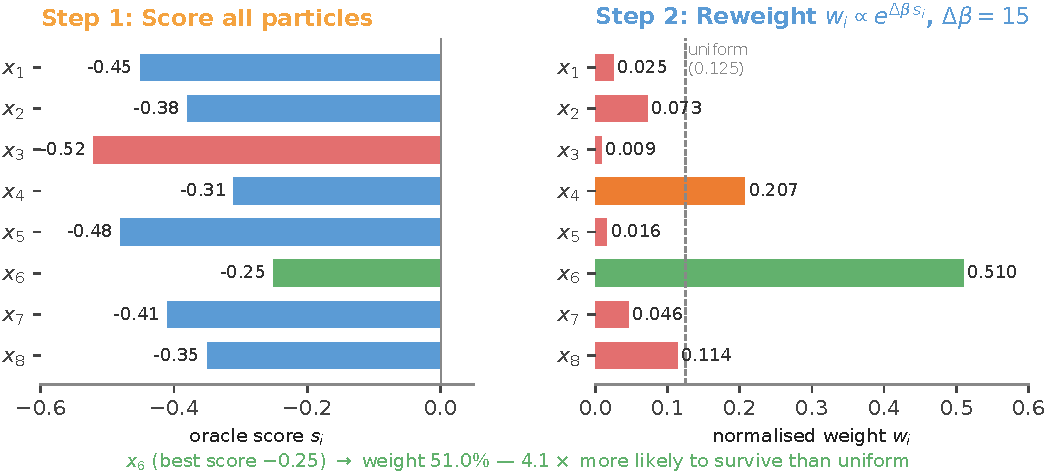
\includegraphics[width=0.95\linewidth]{figures/fig_gpa_walkthrough_score.pdf}
\caption{Score and reweight on the $N\!=\!8$ toy. \textbf{Left:} per-particle oracle scores $s_i$ (best in green: $x_6\!=\!-0.25$; worst in red: $x_3\!=\!-0.52$). \textbf{Right:} normalised weights after the tilt $w_i\!\propto\!\exp(\Delta\beta\,s_i)$ at $\Delta\beta\!=\!15$; uniform $1/N\!=\!0.125$ shown dashed. $x_6$ collects $51.0\%$ of the mass---$4.1\!\times$ the uniform expectation.}
\label{fig:walkthrough-score}
\end{figure}

\subsection{Adapting $\Delta\beta$ via bisection on $\ESS$}

The ESS-adaptive schedule (Lemma~\ref{lem:ess}) chooses $\Delta\beta_t$ so that $\ESS\!\geq\!\alpha N$ \emph{exactly} (not below). With $\alpha\!=\!0.5$, the target is $\ESS_{\rm target}\!=\!4$. Algorithm~\ref{alg:bisect} runs 64 bisection iterations on $[\Delta\beta_{\min}, \Delta\beta_{\max}]\!=\![0,1000]$.

\begin{algorithm}[h]
\caption{Bisection for $\Delta\beta$ given $\ESS$ target}\label{alg:bisect}
\begin{algorithmic}[1]
\State \textbf{Input:} scores $\{r_i\}_{i=1}^N$, target $\tau N$, range $[\Delta\beta_{\min}, \Delta\beta_{\max}]$, max iters $T_{\rm bs}$
\For{$t\!=\!1,\dots,T_{\rm bs}$}
    \State $\Delta\beta_{\rm mid}\!\leftarrow\!(\Delta\beta_{\min}+\Delta\beta_{\max})/2$
    \State $w_i\!\leftarrow\!\exp(\Delta\beta_{\rm mid}\,r_i)/Z$, with $Z\!=\!\sum_j\exp(\Delta\beta_{\rm mid}\,r_j)$
    \State $\ESS\!\leftarrow\!1/\sum_i w_i^2$
    \If{$\ESS > \tau N$} $\Delta\beta_{\min}\!\leftarrow\!\Delta\beta_{\rm mid}$ \Comment{can push harder}
    \Else \;$\Delta\beta_{\max}\!\leftarrow\!\Delta\beta_{\rm mid}$ \Comment{too aggressive}
    \EndIf
\EndFor
\State \textbf{Return:} $\Delta\beta_{\min}$
\end{algorithmic}
\end{algorithm}

For our example, the bisection converges to $\Delta\beta\!\approx\!11.7$, giving $\ESS\!\approx\!4.0\!=\!\alpha N$. The hand-picked $\Delta\beta\!=\!15$ above (which produced $\ESS\!=\!3.08$) was therefore more aggressive than the auto-schedule would choose.

\begin{figure}[h]
\centering
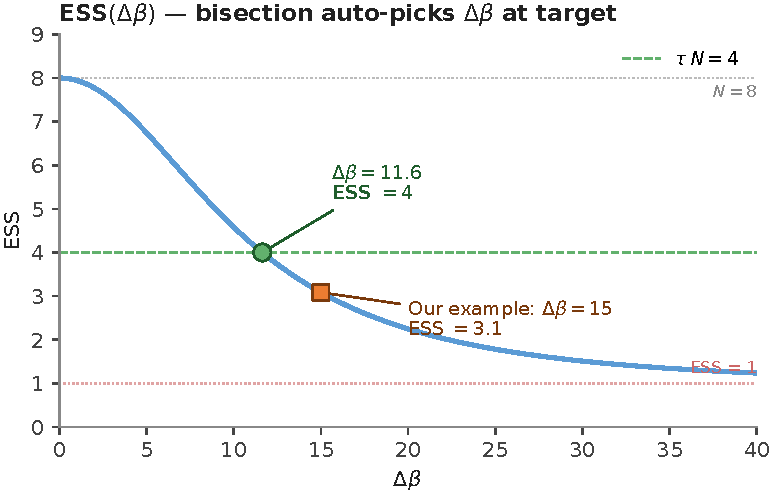
\includegraphics[width=0.78\linewidth]{figures/fig_gpa_walkthrough_ess.pdf}
\caption{$\ESS(\Delta\beta)$ for the $N\!=\!8$ toy oracle scores. The function decreases monotonically from $\ESS\!=\!N$ at $\Delta\beta\!=\!0$ toward $\ESS\!=\!1$ as $\Delta\beta\!\to\!\infty$ (winner-take-all). Bisection finds the unique $\Delta\beta\!=\!11.7$ at which $\ESS$ hits the target $\tau N\!=\!4$ (green dot). The hand-picked $\Delta\beta\!=\!15$ used in the walk-through (orange square) is past the target and so over-collapses the population.}
\label{fig:walkthrough-ess}
\end{figure}

\subsection{Resampling: multinomial vs.\ systematic}

\paragraph{Multinomial.} Draw counts $\!=\!(c_1,\dots,c_N)\!\sim\!\mathrm{Multinomial}(N, w)$. Expected copies per particle are $\E[c_i]\!=\!N\!\cdot\!w_i$, but the realised counts are noisy.

\paragraph{Systematic.} Lay the weights end-to-end as a unit interval $[0,1]$ (segment $i$ has width $w_i$). Drop $N$ pointers at positions $u\!+\!k/N$ for $k\!=\!0,\dots,N\!-\!1$, with $u\!\sim\!\mathrm{Uniform}[0,1/N)$. Particle $i$ receives a number of copies equal to the count of pointers in its segment. This has identical mean to multinomial but lower variance, and is the default in \gpa{}.

For our $N\!=\!8$ example with $u\!=\!0$, the eight pointers at $\{0.000, 0.125, 0.250, 0.375, 0.500, 0.625, 0.750, 0.875\}$ land in segments as follows: $w_2$ (cumulative 0.025--0.098) captures pointer 0.097; $w_4$ (0.107--0.314) captures pointers at 0.125, 0.250; $w_6$ (0.330--0.840) captures pointers at 0.375, 0.500, 0.625, 0.750; $w_8$ (0.886--1.000) captures pointer 0.875. Final copy counts:
\begin{center}
\begin{tabular}{lcccccccc}
\toprule
$i$       & 1 & 2 & 3 & 4 & 5 & 6 & 7 & 8 \\
copies    & 0 & 1 & 0 & 2 & 0 & 4 & 0 & 1 \\
\bottomrule
\end{tabular}
\end{center}
Four particles ($x^1, x^3, x^5, x^7$) are eliminated; $x^6$ is duplicated four times. After resampling, weights reset to $1/N\!=\!0.125$ uniformly.

\begin{figure}[h]
\centering
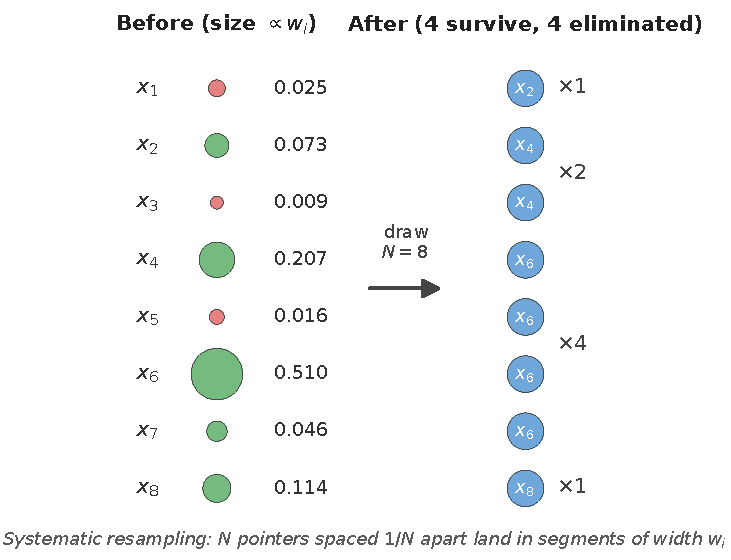
\includegraphics[width=0.85\linewidth]{figures/fig_gpa_walkthrough_resample.pdf}
\caption{Systematic resampling of the $N\!=\!8$ toy. \textbf{Left:} bubble area is proportional to $w_i$; green = retained, red = eliminated by the resampling step. \textbf{Right:} after resampling, all weights reset to $1/N$; $x_6$ now appears four times, $x_4$ twice, $x_2$ and $x_8$ once each. Four particles ($x_1, x_3, x_5, x_7$) are eliminated.}
\label{fig:walkthrough-resample}
\end{figure}

\subsection{Mutation: partial mask + denoise on a length-12 DNA toy}

Each of the eight resampled (now duplicate-rich) particles is independently mutated by $K_\beta$. Concretely, with mask fraction $\mathrm{nf}\!=\!0.25$ ($\!\to\!\lceil 0.25\!\cdot\!12\rceil\!=\!3$ positions on a length-12 sequence):
\begin{center}
\begin{tabular}{ll}
\toprule
\textbf{Step}        & \textbf{Sequence} \\
\midrule
Before (a duplicate of $x^6$)   & \texttt{ACGTATGCACGT} \\
Random mask 3 positions          & \texttt{AC?TA?GC?CGT} \\
Denoise via $p_\theta$           & \texttt{AC\textbf{T}TA\textbf{A}GC\textbf{A}CGT} \\
\midrule
Net edits                         & pos 3: G$\to$T; \, pos 6: T$\to$A; \, pos 9: C$\to$A \\
\bottomrule
\end{tabular}
\end{center}
Two properties this kernel inherits from the pretrained $p_\theta$:
\begin{itemize}
\item \emph{Grammar preservation.} The denoiser sees the unmasked context and proposes tokens consistent with whatever motif/composition rules $p_\theta$ has learned. Random per-position resampling would not.
\item \emph{Diversity restoration.} The four duplicates of $x^6$ each get an \emph{independent} random mask + denoising pass, so they diverge into four distinct child sequences. Without mutation the population would collapse to four identical copies.
\end{itemize}
The mask fraction $\mathrm{nf}$ controls exploration: $\mathrm{nf}\!=\!0.05$ is local search ($\sim\!10$ positions per step on a 200-bp DNA enhancer), $\mathrm{nf}\!=\!0.20$ is large jumps. Section~\ref{sec:results:ablation} reports sensitivity in the practical range.

%-----------------------------------------------------------------------
\section{Hyperparameters}\label{app:hyper}

Table~\ref{tab:hyper-rerd} lists hyperparameters for the SMC-protocol comparison (\drakes{} eval pair); Table~\ref{tab:hyper-ctrldna} lists those for \ctrldna{} comparison (HyenaDNA + gReLU MSE oracles); Table~\ref{tab:hyper-dnacraft} for \dnacraft{} comparison (HyenaDNA/DiMamba + Enformer 50/50). Default values are bolded.

\begin{table}[h]
\caption{Hyperparameters for the SMC-protocol comparison (HepG2 enhancer, MDLM backbone, \drakes{} split-oracle).}
\label{tab:hyper-rerd}
\centering
\small
\begin{tabular}{lll}
\toprule
Parameter & Mean recipe & Spec recipe \\
\midrule
$N$ (population) & 5000 & 5000 \\
$\alpha$ (ESS threshold) & 0.5 & 0.5 \\
$\beta_*$ (target inverse temp) & 200 & 100 \\
$T_{\max}$ (max steps) & 30, hard cap 200 & 30, hard cap 200 \\
nf (mask fraction) & 0.05 & 0.05 \\
DPS gradient strength $\eta$ & 3000 & 3000 \\
$\mathrm{pw}$ (off-target penalty) & 0 & 0.35 \\
GC bio-filter & [0.45, 0.55] & [0.45, 0.55] \\
\bottomrule
\end{tabular}
\end{table}

\begin{table}[h]
\caption{Hyperparameters for \ctrldna{} comparison (Reddy promoters, HyenaDNA backbone, gReLU MSE oracles, universal recipe).}
\label{tab:hyper-ctrldna}
\centering
\small
\begin{tabular}{ll}
\toprule
Parameter & Universal recipe \\
\midrule
$N$ (population) & 10000 \\
$\alpha$ (ESS threshold) & 0.5 \\
$\beta_*$ & 100 \\
$T_{\max}$ (steps) & 60 \\
nf (mask fraction) & 0.05 \\
$K$ (branch factor) & 8 \\
$\mathrm{pw}$ & 0.35 \\
diversity $\lambda$ (conformity) & \textbf{1.0} \\
DPS & off \\
GC bio-filter & off \\
\bottomrule
\end{tabular}
\end{table}

\begin{table}[h]
\caption{Hyperparameters for \dnacraft{} comparison (Gosai 50/50 split, top-128 by MinGap-Eval). C1 = no GC penalty; C3 = soft GC penalty (gct=0.60), no hard bio-filter.}
\label{tab:hyper-dnacraft}
\centering
\small
\begin{tabular}{lll}
\toprule
Parameter & C1 & C3 \\
\midrule
$N$ (population) & 5000 & 5000 \\
$\beta_*$ & 25 & 25 \\
$\mathrm{pw}$ & 0.30 & 0.30 \\
DPS & on & on \\
GC penalty (gct) & --- & 0.60 \\
GC bio-filter & off & off \\
$K$ & 8 & 8 \\
\bottomrule
\end{tabular}
\end{table}

%-----------------------------------------------------------------------
\section{Full GPA-vs-ISM/LEDIDI tables}\label{app:ism_full}

Single-sequence comparison: GPA row = the one sequence in each pool that maximises $\mathrm{AG}-\mathrm{LN}$ (sweet spot: low LN, high held-out AG). Directly comparable to \ism{}/\ledidi{} which are inherently single-sequence.

\begin{table}[h]
\caption{Single-sequence comparison, K562 enhancer, two seeds (uid=181692 natural, uid=50178 random). \gpa{} row = argmax of $\mathrm{AG}-\mathrm{LN}$ within the 5{,}000-seq pool.}
\label{tab:ism_singleseq}
\centering
\small
\begin{tabular}{llrrr}
\toprule
Seed & Method & Edits & LN & AG \\
\midrule
\multirow{4}{*}{uid=181692}
 & \gpa{} (no DPS) uncap   &  96 & 4.97 & \textbf{3.33} \\
 & \gpa{} (+DPS) cap30     &  60 & 6.21 & \textbf{3.47} \\
 & \ism{} gen 115          & 115 & 8.74 & 2.83 \\
 & \ledidi{} t15 $\lambda$=0.05 & 125 & 9.81 & $-$0.22 \\
\midrule
\multirow{4}{*}{uid=50178}
 & \gpa{} (no DPS) cap30   &  60 & 4.71 & 2.75 \\
 & \gpa{} (+DPS) cap30     &  59 & 6.58 & \textbf{3.61} \\
 & \ism{} gen 115          & 115 & 9.58 & 2.92 \\
 & \ledidi{} t15 $\lambda$=0.05 & 105 &11.66 & $-$0.62 \\
\bottomrule
\end{tabular}
\end{table}

\paragraph{Reading the table.}
A single \gpa{} sequence (e.g.\ +DPS cap30 on uid=50178: LN $6.58$, AG $3.61$) beats \ism{} gen 115 on the held-out AG by $+0.69$ at LN $\sim\!3.0$ lower—better held-out activity \emph{and} less reward-hacking. Under any selection rule, \ledidi{} stays AG-negative; not one of its 50 reruns produces an AG-positive sequence.

\paragraph{Apples-to-apples runtime (single H100, K562 enhancer, 5{,}000-sequence pool).}
Table~\ref{tab:ism_runtime} reports wall-time at matched output volume, averaged across the random and natural pools. \gpa{} is fully population-parallel: a single SMC step propagates all 5{,}000 particles together through the diffusion proposal, so the per-particle cost is the GPU-memory chunk \texttt{mutation\_batch\_size=128} amortised over the population. \ism{} is also nominally population-parallel (5{,}000 independent greedy trajectories), but its sequential cost is fixed at 115 generations per seed, and that dominates wall regardless of how memory chunks are batched. \ledidi{} is chunked-sequential by design: 5{,}000 seeds processed in 39 chunks of 128 along the Gumbel-softmax optimisation. The result is $\sim\!9.3\times$ speedup over \ism{} and $\sim\!3.4\times$ speedup over \ledidi{} at identical pool size and identical hardware.

\begin{table}[h]
\caption{Apples-to-apples runtime: single H100, 5{,}000-sequence K562-enhancer pool, averaged across random and natural seed pools. \gpa{} = v3 noDPS recipe (matches Sec.~\ref{sec:results:ism}). Speedup column is $\mathrm{wall}_{\text{baseline}}/\mathrm{wall}_{\gpa{}}$.}
\label{tab:ism_runtime}
\centering
\small
\begin{tabular}{lllr}
\toprule
Method & Wall (5K pool) & Parallelism & Speedup vs.\ \gpa{} \\
\midrule
\textbf{\gpa{}} & \textbf{$\sim\!11.6$ min} & population-parallel (5{,}000 SMC particles) & --- \\
\ledidi{}       & $\sim\!40$ min     & chunked-sequential (39 chunks $\times$ 128 seeds) & $\sim\!3.4\times$ slower \\
\ism{}          & $\sim\!107.5$ min  & population-parallel, but 115 sequential greedy gens & $\sim\!9.3\times$ slower \\
\bottomrule
\end{tabular}
\end{table}

%-----------------------------------------------------------------------
\section{Full DNA-CRAFT tables (GPA-C1 vs GPA-C3)}\label{app:dnacraft_full}

The headline column in Table~\ref{tab:dnacraft} uses GPA-C3 (\texttt{dps\_pw030\_b25\_gct060\_nobio}). This appendix shows the same benchmark with the alternate recipe variant GPA-C1 (\texttt{dps\_pw030\_b25}, no GC penalty), under the matched-output-budget protocol of Table~\ref{tab:dnacraft} (\texttt{by\_pool\_composite} top-64 from \texttt{gpa\_output\_best\_eval.h5}, 3 reps for both variants). Both variants run at $\sim\!3.6$ min/seed (no MCTS) on the MDLM backbone; the only difference is the soft GC-centering term added to C3's DPS gradient.

\paragraph{Recipe decomposition.}
Each token in the recipe name maps to a specific knob in the GPA algorithm of \S\ref{sec:method}, with no other differences between the two variants:
\begin{itemize}
\item \texttt{dps} -- enables the Gumbel-softmax oracle gradient with strength $\eta\!=\!3000$ (\S\ref{sec:method:ext}, ``Gumbel-softmax oracle gradient (DPS)''). This is a biased proposal in the sense of \S\ref{sec:method:ext} and is shared by both C1 and C3, so the C1$\leftrightarrow$C3 contrast does not move along the DPS-bias axis.
\item \texttt{pw030} -- sets the off-target weight $\mathrm{pw}\!=\!0.30$ in the linear fitness of Eq.~\ref{eq:fitness} (\S\ref{sec:method:pw}); the same $0.30$ weights the off-target term inside the DPS gradient as well.
\item \texttt{b25} -- sets the SMC tilt ceiling $\beta_*\!=\!25$. This is below the default range $\beta_*\!\in\!\{100,200\}$ in \S\ref{sec:exp} and is a deliberately gentler tilt that preserves population diversity at some cost in MinGap; both variants share it.
\item \texttt{gct060} \emph{(C3 only)} -- adds a quadratic centering term $-w\,(g(x)-0.60)^2$ to the DPS objective before backpropagation, where $g(x)\!=\!\overline{P(C)+P(G)}$ is the per-position soft-onehot GC fraction and $w\!=\!10$. The penalty rides inside the same Gumbel-softmax gradient that DPS already computes; it is \emph{not} a hard accept/reject filter.
\item \texttt{nobio} -- disables the hard bio-filter (no \texttt{gc\_low}/\texttt{gc\_high} interval gating). All GC discipline in C3 therefore comes from the soft \texttt{gct060} term in the DPS gradient.
\end{itemize}
Both variants additionally use the default branch factor $K\!=\!8$ (\S\ref{sec:method:ext}, Prop.~\ref{prop:K}) and population $N\!=\!5{,}000$ (Table~\ref{tab:dnacraft} caption), so both target $\pi_{\beta_*}^{(K=8)}\!\neq\!\pi_{\beta_*}$ in the sense of Prop.~\ref{prop:K}; the C1$\leftrightarrow$C3 contrast isolates the GC-centering term with $K$, $\beta_*$, $\mathrm{pw}$, $N$, and the DPS bias all held constant.

\begin{table}[h]
\caption{\dnacraft{} benchmark with the GPA-C1 alternate recipe (\texttt{dps\_pw030\_b25}; no GC penalty), reported alongside the headline GPA-C3 (Table~\ref{tab:dnacraft}). Both columns: \texttt{by\_pool\_composite} top-64 from \texttt{gpa\_output\_best\_eval.h5}, mean (std) over 3 reps. Baselines verbatim from \citet{dnacraft2026}.}
\label{tab:dnacraft_full_eval}
\centering
\scriptsize
\begin{tabular}{llcccccccccc}
\toprule
Cell & Metric & SMC & CG & TDS & DRAKES & D3 & Ledidi & Ctrl-DNA & DNA-CRAFT & \gpa{}-C1 & \gpa{}-C3 \\
\midrule
\multirow{4}{*}{HepG2}
 & MinGap   & 1.61 & $-$0.23 & 0.40 & $-$1.40 & 0.05 & 5.77 & \textbf{7.79} & 4.35 & 6.87 & 6.91 \\
 & Motif    & 0.55 & 0.86 & 0.40 & 0.06 & 0.87 & 0.58 & 0.63 & \textbf{0.92} & 0.90 & \textbf{0.92} \\
 & 3-mer    & 0.81 & 0.97 & 0.74 & $-$0.36 & \textbf{0.98} & 0.76 & 0.49 & \textbf{0.98} & 0.95 & 0.95 \\
 & Diversity& 0.83 & \textbf{1.98} & 0.96 & 1.86 & \textbf{1.98} & \textbf{1.98} & 1.90 & \textbf{1.98} & 1.81 & 1.86 \\
\midrule
\multirow{4}{*}{K562}
 & MinGap   & 4.12 & 0.00 & 1.62 & $-$0.20 & 0.18 & 7.66 & \textbf{9.07} & 5.69 & 8.18 & 8.13 \\
 & Motif    & 0.45 & 0.85 & 0.51 & 0.14 & 0.86 & 0.65 & 0.63 & 0.93 & 0.93 & \textbf{0.94} \\
 & 3-mer    & 0.66 & 0.94 & 0.65 & $-$0.35 & 0.96 & 0.69 & 0.41 & \textbf{0.98} & 0.92 & 0.95 \\
 & Diversity& 0.31 & \textbf{1.98} & 0.64 & 1.96 & \textbf{1.98} & \textbf{1.98} & 1.90 & \textbf{1.98} & 1.56 & 1.83 \\
\midrule
\multirow{4}{*}{SK-N-SH}
 & MinGap   & 0.56 & $-$0.28 & 0.19 & 0.09 & $-$0.01 & 3.03 & 3.72 & 3.23 & \textbf{5.07} & 4.98 \\
 & Motif    & 0.52 & 0.86 & 0.48 & 0.23 & 0.84 & 0.38 & 0.48 & 0.88 & 0.89 & \textbf{0.92} \\
 & 3-mer    & 0.78 & 0.95 & 0.72 & $-$0.38 & 0.93 & 0.37 & 0.20 & \textbf{0.97} & 0.87 & 0.94 \\
 & Diversity& 1.27 & \textbf{1.98} & 0.92 & 1.83 & 1.97 & \textbf{1.98} & 1.86 & \textbf{1.98} & 1.59 & 1.86 \\
\bottomrule
\end{tabular}
\end{table}

\paragraph{Reading.}
GPA-C1 and GPA-C3 give nearly tied MinGap and Motif Spearman on every cell (within seed std on most rows). C3 wins Motif on HepG2 / K562 / SK-N-SH ($+0.02$/$+0.01$/$+0.03$) and 3-mer on K562 / SK-N-SH ($+0.03$/$+0.07$). The biggest practical difference is Diversity: the soft GC-centering term in C3's DPS gradient recovers $+0.05$ to $+0.27$ Shannon bits over C1 on every cell, lifting C3 above the Ctrl-DNA Diversity floor on all three cells. The mechanism is indirect: by penalising drift away from $g(x)\!=\!0.60$ at every Gumbel-softmax step, the term blunts the oracle's tendency to push particles toward narrow high-GC modes, which in turn keeps the population spread out in sequence space. C1 wins MinGap on K562 / SK-N-SH ($+0.05$/$+0.09$) but loses across the rest. C3 is the headline because the +Diversity / +Motif / +3-mer trade dominates the small MinGap give-back; C1 is reported as an ablation that isolates the GC-penalty's contribution.

\paragraph{Backbone caveat.}
\dnacraft{}'s reported numbers in Table~\ref{tab:dnacraft} are obtained on a Mamba-style discrete-diffusion (DiMamba) backbone whose code and pretrained checkpoints are not publicly available; the same paper also reports DiMamba-vs-MDLM ablations that show DiMamba contributes additional biological-faithfulness gains. Our \gpa{}-C1 / \gpa{}-C3 numbers are obtained on the publicly available MDLM backbone of \citet{sahoo2024mdlm} and should be read as a lower bound on what \gpa{} would achieve at backbone parity, by Remark~\ref{rem:agnostic}.

%-----------------------------------------------------------------------
\section{Wall-time table}\label{app:wall}

\begin{table}[h]
\caption{Wall time per seed and 5-seed totals (HepG2, identical H100 hardware, identical HyenaDNA backbone). Wall time excludes downstream motif scoring.}
\label{tab:wall}
\centering
\small
\begin{tabular}{lrr}
\toprule
Method & Wall/seed (h) & 5-seed total (GPU-h) \\
\midrule
\ctrldna{} R200 (RL fine-tune) & $43.5\pm 0.8$ & $\sim\!218$ \\
\gpa{} v3 (K=8, no diversity)  & $3.97\pm 0.59$ & 19.8 \\
\gpa{} v4 (K=8 + rejuvenation) & $2.17\pm 0.22$ & 10.8 \\
\gpa{} v5 (K=8 + diversity)    & $\mathbf{2.22\pm 0.52}$ & $\mathbf{11.1}$ \\
\bottomrule
\end{tabular}
\end{table}

%-----------------------------------------------------------------------
\section{DPS gradient ablation}\label{app:dps_ablation}

Population annealing alone (no DPS) already beats single-chain refinement baselines; DPS gradient is a multiplicative enhancement.

\begin{table}[h]
\caption{DPS gradient ablation on Gosai HepG2.}
\label{tab:dps_ablation}
\centering
\small
\begin{tabular}{llrrr}
\toprule
Track & Metric & \gpa{}-only & \gpa{}+DPS & $\Delta$(DPS) \\
\midrule
Mean & $H_{\mathrm{eval}}$ & $8.73\pm 0.50$ & $\mathbf{10.06\pm 0.19}$ & $+1.33$ \\
Mean & Spec & 1.58 & 3.06 & $+1.48$ \\
Spec & $H_{\mathrm{eval}}$ & $8.28\pm 0.12$ & $9.35\pm 0.20$ & $+1.07$ \\
Spec & Spec & $6.11\pm 1.45$ & $\mathbf{7.61\pm 0.25}$ & $+1.50$ \\
\bottomrule
\end{tabular}
\end{table}

%-----------------------------------------------------------------------
\section{Naturalness audit}\label{app:naturalness}

\begin{table}[h]
\caption{Naturalness audit (HepG2 top-128). \gpa{} produces bio-plausible sequences by construction; \ctrldna{} reward-hacks to non-biological space.}
\label{tab:nat}
\centering
\small
\begin{tabular}{lrrr}
\toprule
Metric & Real (Gosai) & \gpa{} & \ctrldna{} \\
\midrule
GC mean & 0.44 & 0.41 & 0.45 \\
\textbf{bio\_pass\_rate} & 0.51 & $\mathbf{1.00}$ & $\mathbf{0.05}$ \\
max homopolymer & 5.4 & 5.1 & $\mathbf{20.9}$ \\
$k$=3 Pearson & 1.0 & 0.61 & 0.39 \\
HNF1A enrichment & $0\times$ & $10\,040\times$ & $7\,812\times$ \\
\bottomrule
\end{tabular}
\end{table}

\begin{figure}[h]
\centering
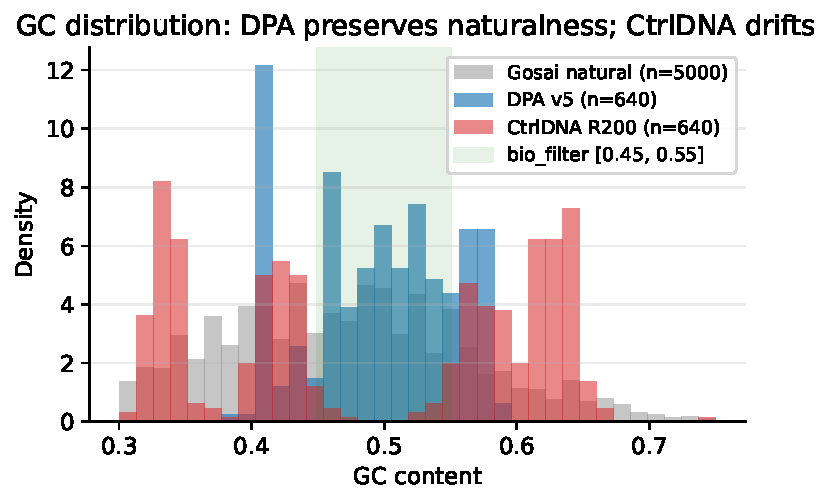
\includegraphics[width=0.6\linewidth]{figures/fig2_gc.pdf}
\caption{GC distribution comparison on HepG2 top-128 sequences. \gpa{} (blue) clusters near the lower edge of the bio-filter (45\%) but stays within the natural Gosai range (gray); \ctrldna{} (red) drifts widely, with a heavy tail of low- and high-GC sequences and a substantial fraction outside the natural distribution.}
\label{fig:gc}
\end{figure}

%-----------------------------------------------------------------------
\section{Extreme specificity}\label{app:extreme}

Pushing $\mathrm{pw}$ beyond the canonical $0.35$ trades $H_{\mathrm{eval}}$ for higher specificity until both off-targets fall below baseline (Table~\ref{tab:extreme}).

\begin{table}[h]
\caption{Extreme-specificity extension on Gosai HepG2 (single run each, $N\!=\!5000$).}
\label{tab:extreme}
\centering
\small
\begin{tabular}{rrrrr}
\toprule
$\mathrm{pw}$ & $H_{\mathrm{eval}}$ & $K_{\mathrm{eval}}$ & $S_{\mathrm{eval}}$ & $H{>}8 \wedge K{<}0 \wedge S{<}0$ \\
\midrule
0.35 & 9.65 & 2.15 &  1.10 & 0 \\
0.50 & 9.54 & 1.96 &  0.63 & 0 \\
0.70 & 8.73 & 1.52 &  0.35 & 0 \\
1.00 & 8.57 & 0.69 & $-$0.48 & 26 \\
1.50 & $\mathbf{8.44}$ & 0.55 & $\mathbf{-0.66}$ & $\mathbf{54}$ \\
\bottomrule
\end{tabular}
\end{table}

\paragraph{Beta trajectory.}
Figure~\ref{fig:beta} shows a representative ESS-adaptive $\beta$ trajectory and the population-mean reward over SMC steps for a HepG2 run.

\begin{figure}[h]
\centering
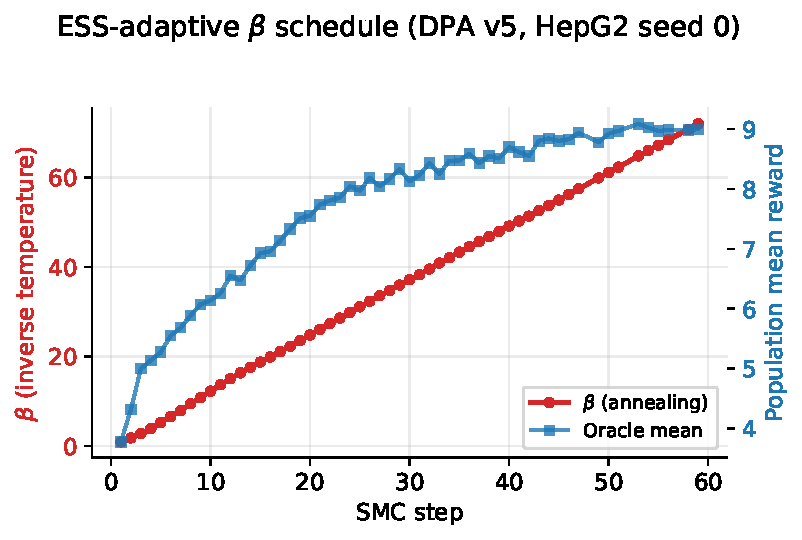
\includegraphics[width=0.6\linewidth]{figures/fig4_beta_traj.pdf}
\caption{Representative \gpa{} run trajectory (HepG2, seed 0). Red trace: ESS-adaptive $\beta$ schedule rises through the annealing path. Blue trace: population mean reward grows monotonically toward saturation as $\beta$ increases.}
\label{fig:beta}
\end{figure}

%-----------------------------------------------------------------------
\section{Negative result: APF correction for $\epsilon$-greedy $K$-branching}\label{app:apf}

A natural attempt to recover Shannon under $K$-branching is to soften the argmax with $\epsilon$-greedy ($\tau\!>\!0$ softmax over the $K$ siblings) and apply the auxiliary-particle-filter weight correction \citep{pittshephard1999}:
\[
w_{\mathrm{new}} = w_{\mathrm{old}}\big/p_\tau(\mathrm{winner}),\qquad p_\tau(j)=\exp(r_j/\tau)\big/\sum_m\exp(r_m/\tau).
\]
Compute the expectation:
\[
\E[w_{\mathrm{new}}\,\varphi(x_{\mathrm{winner}})] = \E_{x_{1:K}\sim q}\!\!\left[\sum_{j=1}^K \frac{\exp(r_j/\tau)}{\sum_m\exp(r_m/\tau)}\cdot\frac{\sum_m\exp(r_m/\tau)}{K\exp(r_j/\tau)}\,\varphi(x_j)\right]=\frac{1}{K}\sum_j \E_q[\varphi(x_j)],
\]
i.e.\ the corrected estimator is equivalent to a single-child sample. The $K$ siblings collapse and the effective-$\beta$ boost vanishes. Empirically, on a synthetic linear reward $r(x)\!=\!3x$ with $q$ uniform on $[0,1]$ (200K Monte-Carlo trials):
\begin{center}
\small
\begin{tabular}{lrrr}
\toprule
Variant & $\E[x]$ & $\mathrm{Var}[x]$ & ESS \\
\midrule
$K=1$ no selection                & 0.5000 & 0.0833 & 100.0\% \\
$K=8$ argmax (no correction)      & 0.8887 & 0.0099 & 100.0\% \\
$K=8$ softmax $\tau\!=\!0.3$ (no corr.) & 0.8445 & 0.0180 & 100.0\% \\
\textbf{$K=8$ softmax $\tau\!=\!0.3$ + APF} & 0.4880 & 0.0874 & 0.4\% \\
$K=8$ softmax $\tau\!=\!1.0$ + APF & 0.5009 & 0.0829 & 53.1\% \\
\bottomrule
\end{tabular}
\end{center}
ESS collapses at low $\tau$ and the corrected mean/variance reproduces $K=1$. We therefore do \emph{not} use APF correction for production runs and report only argmax $K$-branching. K-annealing schedules and waste-free SMC \citep{dau2022wastefree} remain valid theoretical alternatives, deferred to future work.

%-----------------------------------------------------------------------
\section{Negative result: post-hoc Metropolis tempering}\label{app:posthoc}

Another natural Shannon-rescue move is to load the concentrated argmax-$K$ pool and run Metropolis–Hastings at lower $\beta'$ to spread the population. We tested this on the K562 promoter pool (50 MH steps, nf=0.05, HyenaDNA proposal):

\begin{center}
\small
\begin{tabular}{rrrrr}
\toprule
$\beta'$ & accept rate & $\Delta$comp & $\Delta$tgt & $\Delta H$ \\
\midrule
25 &  3.4\% & $+0.02$ & $-0.06$ & $+0.05$ \\
12 &  6.5\% & $-0.15$ & $-0.27$ & $+0.10$ \\
 6 & 13.1\% & $-0.68$ & $-0.77$ & $+0.21$ \\
 3 & 29.1\% & $-2.12$ & $-2.22$ & $+0.39$ \\
 1 & 73.7\% & $-4.71$ & $-5.35$ & $+0.61$ \\
\bottomrule
\end{tabular}
\end{center}
The Pareto slope is $\sim\!3\!-\!5$ target units per $0.1$ nat of Shannon, far too steep for the diversity gap to \dnacraft{}/\ctrldna{} K562 ($\sim\!0.5$ nat) to be closed without erasing the target advantage. Increasing chain length or shrinking nf does not change the local-neighborhood geometry. The honest reading: under sharply peaked oracles, the activity–diversity tension is in the reward landscape, not the sampler.

%-----------------------------------------------------------------------
\section{GC distribution and floor-hugging}\label{app:gc}

Even with the bio-filter $\mathrm{GC}\!\in\![0.45,0.55]$, $60\!-\!75\%$ of \gpa{} top-128 sequences cluster at the lower bound. Two facts:
\begin{enumerate}
\item This is a property of the \emph{masked-diffusion proposal} at low noise fraction. At $\mathrm{nf}\!=\!0.20$ the bias inverts toward the upper bound (GC $\approx\!0.54$); the crossover occurs near $\mathrm{nf}\!\approx\!0.16\!-\!0.17$.
\item The eval oracle is GC-agnostic: at both $\mathrm{nf}$ extremes, top-128 oracle scores are comparable. The GC bias arises from $p_\theta$, not from the reward signal.
\end{enumerate}
Three mitigations were tested with mixed success: (i) GC-aware DPS gradient (\verb|gc_dps_weight|) reduces floor-hugging from $61.5\%$ to $55.0\%$ at $-0.09$ $H_{\mathrm{eval}}$ cost; (ii) narrow $1\%$ GC bands achieve uniform GC by construction at $-0.25$ $H_{\mathrm{eval}}$; (iii) stratified resampling within $2\%$ GC bins \citep{verge2015island} achieves balanced coverage at $-0.50$ to $-1.0$ $H_{\mathrm{eval}}$. We report all three options in the codebase but use the unmitigated baseline in the headline tables for fair comparison with peer methods.

%-----------------------------------------------------------------------
\section{Ctrl-DNA enhancer comparison (V7 main + V5/V8 ablations)}\label{app:ctrldna_enhancer}

This appendix gives the dedicated \ctrldna{}-vs-\gpa{} enhancer comparison referenced in \S\ref{sec:results:promoter}. Same Gosai 50/50 split as the \dnacraft{} benchmark, top-128 selection per cell, 5 \gpa{} seeds. The headline GPA recipe is V7 (universal: $K\!=\!8$, diversity $\lambda\!=\!1.0$); V8a, V8b (alternative pairwise-suppression formulations) and V5 (the previous default with $\lambda\!=\!0.2$) are ablations.

\begin{table}[h]
\caption{Ctrl-DNA vs.\ \gpa{} on Gosai HepG2/K562/SKNSH enhancers (5 seeds; mean (std)). Headline = V7 universal recipe; V8a (log\_ratio + pw=1.0), V8b (linear + pw=1.0) and V5 ($\lambda\!=\!0.2$) are ablations of the diversity / pairwise-suppression knob. \texttt{target\_raw} = mean target oracle score; \texttt{ΔR} = normalised target minus mean off-target; \texttt{shannon} = per-position entropy; \texttt{motif\_corr} = FIMO Pearson against per-cell real reference.}
\label{tab:ctrldna_enhancer}
\centering
\footnotesize
\setlength{\tabcolsep}{4pt}
\begin{tabular}{llrrrr}
\toprule
Cell & Method & target\_raw $\uparrow$ & ΔR $\uparrow$ & shannon $\uparrow$ & motif\_corr $\uparrow$ \\
\midrule
\multirow{5}{*}{HepG2}
 & \ctrldna{} R200             & 5.32 (0.65) & 0.48 (0.10) & 1.65 (0.14) & \textbf{0.29} (0.16) \\
 & \gpa{} V5 ($K\!=\!8, \lambda\!=\!0.2$) & 9.86 (0.10) & 0.85 (0.01) & 1.49 (0.03) & 0.19 (0.03) \\
 & \gpa{} V7 ($K\!=\!8, \lambda\!=\!1.0$) & \textbf{9.90} (0.12) & 0.84 (0.02) & 1.59 (0.11) & 0.20 (0.02) \\
 & \gpa{} V8a (log\_ratio, pw=1.0) & 6.61 (0.04) & 0.68 (0.01) & \textbf{1.93} (0.00) & 0.15 (0.02) \\
 & \gpa{} V8b (linear, pw=1.0) & 9.51 (0.10) & \textbf{0.93} (0.02) & 1.70 (0.11) & 0.10 (0.04) \\
\midrule
\multirow{5}{*}{K562}
 & \ctrldna{} R200             & \textbf{9.99} (1.52) & \textbf{0.77} (0.14) & 1.60 (0.15) & 0.24 (0.07) \\
 & \gpa{} V5 ($K\!=\!8, \lambda\!=\!0.2$) & 8.82 (0.13) & 0.34 (0.00) & 1.43 (0.09) & \textbf{0.26} (0.02) \\
 & \gpa{} V7 ($K\!=\!8, \lambda\!=\!1.0$) & 8.83 (0.12) & 0.32 (0.01) & 1.65 (0.02) & 0.24 (0.02) \\
 & \gpa{} V8a (log\_ratio, pw=1.0) & 6.48 (0.03) & 0.39 (0.01) & \textbf{1.94} (0.01) & 0.24 (0.01) \\
 & \gpa{} V8b (linear, pw=1.0) & 8.15 (0.04) & 0.41 (0.01) & 1.68 (0.02) & 0.25 (0.02) \\
\midrule
\multirow{5}{*}{SK-N-SH}
 & \ctrldna{} R200             & 9.93 (1.13) & \textbf{0.71} (0.10) & 1.63 (0.17) & \textbf{0.23} (0.10) \\
 & \gpa{} V5 ($K\!=\!8, \lambda\!=\!0.2$) & \textbf{14.33} (0.20) & 0.10 (0.01) & 1.49 (0.04) & \textbf{0.23} (0.01) \\
 & \gpa{} V7 ($K\!=\!8, \lambda\!=\!1.0$) & 14.17 (0.18) & 0.10 (0.00) & 1.63 (0.04) & 0.20 (0.01) \\
 & \gpa{} V8a (log\_ratio, pw=1.0) & 6.29 (0.08) & 0.22 (0.01) & \textbf{1.91} (0.01) & 0.15 (0.01) \\
 & \gpa{} V8b (linear, pw=1.0) & 8.26 (0.15) & 0.29 (0.03) & 1.74 (0.05) & 0.10 (0.01) \\
\bottomrule
\end{tabular}
\end{table}

\paragraph{Headlines.}
\gpa{} V7 (the universal recipe) wins target\_raw on HepG2 and SK-N-SH ($+4.58$ and $+4.24$ over \ctrldna{}), and is competitive on K562 within $\sim$1 std. \ctrldna{} retains a ΔR (specificity) edge on K562 and SK-N-SH at the cost of $\sim$50\% lower target activity on HepG2/SK-N-SH and high seed-to-seed variance ($\pm 1.13$--$1.52$). The V7 vs.\ V5 comparison shows the diversity-$\lambda$ bump (from $0.2$ to $1.0$) buys $+0.10$--$0.22$ shannon on every cell at zero target cost, isolating the population-conformity penalty as a strict Pareto improvement. V8a/V8b are alternative pairwise-suppression formulations: V8a (log-ratio reward, pw=1.0) achieves the tightest shannon ($1.91$--$1.94$, near uniform) but at substantial target cost; V8b (linear, pw=1.0) recovers HepG2/K562 target while maximising HepG2 ΔR. The four GPA variants together trace a Pareto front in (target, shannon, motif) space at fixed inference cost---one knob per recipe, no retraining.

%-----------------------------------------------------------------------
\section{DNA-CRAFT $K$ and $i$ scaling sweeps (UCB-MCTS variant)}\label{app:ucb_scaling}

\paragraph{Why MCTS at all.}
DNA-CRAFT replaces the SMC population with a single depth-bounded Monte Carlo Tree Search loop on a DiMamba diffusion backbone, and shows that this delivers state-of-the-art motif and 3-mer grammar fidelity on the Gosai enhancer benchmark (Table~\ref{tab:dnacraft}). The mechanism that delivers their grammar bar is plausible on its face: tree search amortises the cost of choosing the right next mutation by replaying the same scoring oracle across multiple competing children before committing—a strictly more informed proposal than picking the first child that scores well. \gpa{}'s standard $K$-branch is a depth-1 special case of this idea: try $K$ candidates from the proposal and keep the best (Sec.~\ref{sec:method:ext}). It is natural to ask whether the same \emph{deeper} planning that powers \dnacraft{}'s grammar—expanding the best leaves over multiple iterations rather than just one---closes \gpa{}'s residual gap to \dnacraft{} on motif/3-mer correlation. The \texttt{ucb\_stacked} variant exists to test exactly that question.

\paragraph{What \texttt{ucb\_stacked} does, step by step.}
At every SMC mutation step, each particle $x_t^{(j)}$ becomes the root of an independent Monte Carlo tree. We then run $i$ iterations on that tree, where each iteration follows the standard four-phase MCTS-with-UCB1 loop \citep[``UCT'';][]{kocsis2006uct}:
\begin{enumerate}
\item \emph{Selection.} Traverse from the root to a leaf by greedily picking, at each internal node $v$ with already-expanded children $\{a\}$, the child that maximises the UCB1 score \citep{auer2002ucb,kocsis2006uct}
\begin{equation}\label{eq:ucb1}
    \mathrm{UCB1}(a) \;=\; \bar{Q}(a) \;+\; c\sqrt{\frac{\ln n(v)}{n(a)}},
\end{equation}
where $\bar{Q}(a)\!\in\![0,1]$ is the mean (range-normalised) reward backed up through child $a$, $n(a)$ is the visit count of $a$, $n(v)\!=\!\sum_a n(a)$ is the parent visit count, and $c\!=\!\sqrt{2}$ is the standard exploration constant. The first term exploits children with high empirical value; the second term explores low-visit children with a $\sqrt{\log n / n(a)}$ confidence radius. Together this is the canonical bandit rule of \citet{auer2002ucb} for stochastic multi-armed bandits, and \citet{kocsis2006uct} show that applying it node-wise inside a tree (UCT) inherits the same $\mathcal{O}(\log n)$ regret bound at each node. Children with $n(a)\!=\!0$ are tried first by convention so the second term remains well-defined.
\item \emph{Expansion.} Apply \gpa{}'s standard $K$-branch operator at the selected leaf: draw $K\!=\!8$ children using partial-mask$\circ$denoise + DPS (the same operator the no-MCTS \gpa{} would use as its mutation kernel).
\item \emph{Evaluation.} Score each new child under the eval-side reward.
\item \emph{Backpropagation.} Update visit counts $n(\cdot)$ and value estimates $\bar{Q}(\cdot)$ along the path from each new child up to the root, so the next iteration's UCB1 selection (Eq.~\ref{eq:ucb1}) uses fresh statistics.
\end{enumerate}
We bound the tree depth at $d\!=\!2$, so the planner looks at most two mutation steps ahead. After $i$ iterations the tree has at most $1\!+\!i\!\cdot\!K$ nodes; the mutated state for $x_t^{(j)}$ is the highest-reward leaf in that tree. The SMC step then proceeds as usual: the new particle states are importance-weighted at the next $\beta$, resampled if $\ESS$ degenerates, and the loop continues.

\paragraph{Connection to \dnacraft{}.}
The four-step loop (UCB selection $\to$ $K$-fold expansion $\to$ scoring $\to$ reward backprop) is identical in shape to \dnacraft{}'s tree search. What differs is the \emph{scope} of where the tree sits and how it is consumed:
\begin{itemize}
\item \dnacraft{} runs \emph{one} MCTS for the whole design problem: $N_{\mathrm{iter}}\!=\!64$ iterations, $M\!=\!128$ children per expansion, full leaf-to-clean rollouts. Their MinGap-Set archive accumulates the best $N_{\max}\!=\!64$ leaves seen during the run, and that archive is the output (no SMC, no population).
\item \texttt{ucb\_stacked} runs \emph{many} MCTSs: one per particle, per SMC step. Each tree is run for $i\!\in\!\{12,18,24,36\}$ iterations with $K\!=\!8$ children per expansion at depth $d\!=\!2$, no full rollouts (we score after one denoising step). The output is the SMC population at the final $\beta$, exactly as in standard \gpa{}; the trees are only the per-particle mutation kernel.
\end{itemize}
``Stacked'' refers to the layering: MCTS sits \emph{on top of} the $K$-branch+DPS proposal in the SMC inner loop. The $K$-branch supplies the unit of expansion; UCB1+depth-2 lookahead is the planner that decides which leaf is worth expanding next. In effect, \texttt{ucb\_stacked} is a way to ask: does \dnacraft{}'s planning shape, used as a mutation kernel inside SMC, give us the same grammar advantages \dnacraft{} reports as the entire search?

\paragraph{Cost.}
Each \texttt{ucb\_stacked} mutation step performs $1\!+\!i\!\cdot\!K$ scoring calls per particle (vs.\ standard \gpa{}'s 8). At our default $K\!=\!8, i\!=\!18$ this is $145$ scoring calls per particle per step---roughly $18\!\times$ the standard \gpa{} mutation budget. The wallclock overhead is sub-linear in both axes (we report the empirical scaling laws below); for the $i\!=\!18$ headline configuration this works out to $\sim\!7\!\times$ the standard \gpa{}-C3 wallclock per seed.

\paragraph{What the tables below show.}
The two sweeps below sit on K562 and fix one axis at the pilot value while sweeping the other ($K\!=\!8$ for the $i$-sweep, $i\!=\!12$ for the $K$-sweep), at depth $d\!=\!2$ throughout. Wallclock is per seed on a single H100; all metrics are reported under the matched-output-budget protocol of Table~\ref{tab:dnacraft} (\texttt{by\_pool\_composite} top-64 from \texttt{gpa\_output\_best\_eval.h5}). Both sweeps include the standard $K\!=\!8, i\!=\!12$ pilot anchor (5 seeds) for cross-reference.

\begin{table}[h]
\caption{DNA-CRAFT $i$-axis sweep (K562, $K\!=\!8$, $d\!=\!2$). \texttt{by\_pool\_composite} top-64. 5 seeds for $i\!\in\!\{12,18\}$, 2 seeds for $i\!\in\!\{24,36\}$.}
\label{tab:ucb_i_sweep}
\centering
\small
\begin{tabular}{rrrrrrr}
\toprule
$i$ & $n$ & wall (min) & MinGap & Motif & 3-mer & Diversity \\
\midrule
12 & 5 & 31.35 (3.62) & $+$8.066 (0.063) & 0.940 (0.004) & 0.945 (0.023) & 1.903 (0.022) \\
18 & 5 & 32.26 (0.62) & $+$8.115 (0.013) & 0.942 (0.003) & 0.961 (0.003) & 1.926 (0.027) \\
24 & 2 & 37.07 (4.08) & $+$8.153 (0.075) & 0.940 (0.002) & 0.968 (0.003) & 1.941 (0.012) \\
36 & 2 & 46.60 (3.23) & $+$8.015 (0.001) & 0.941 (0.003) & 0.965 (0.002) & 1.937 (0.014) \\
\bottomrule
\end{tabular}
\end{table}

\begin{table}[h]
\caption{DNA-CRAFT $K$-axis sweep (K562, $i\!=\!12$, $d\!=\!2$). \texttt{by\_pool\_composite} top-64. 5 seeds for $K\!=\!8$ (pilot anchor), 2 seeds for $K\!\in\!\{16,24,32\}$.}
\label{tab:ucb_K_sweep}
\centering
\small
\begin{tabular}{rrrrrrr}
\toprule
$K$ & $n$ & wall (min) & MinGap & Motif & 3-mer & Diversity \\
\midrule
 8 & 5 & 31.35 (3.62) & $+$8.066 (0.063) & 0.940 (0.004) & 0.945 (0.023) & 1.903 (0.022) \\
16 & 2 & 49.39 (6.64) & $+$8.124 (0.108) & 0.939 (0.002) & 0.959 (0.008) & 1.898 (0.043) \\
24 & 2 & 69.00 (13.13) & $+$8.070 (0.016) & 0.942 (0.004) & 0.953 (0.007) & 1.935 (0.008) \\
32 & 2 & 77.40 (4.31) & $+$8.022 (0.103) & 0.936 (0.000) & 0.953 (0.002) & 1.907 (0.045) \\
\bottomrule
\end{tabular}
\end{table}

\paragraph{Reading.}
Wallclock is sub-linear in both axes ($\mathrm{wall}\propto i^{0.369}$, $R^2\!=\!0.91$; $\mathrm{wall}\propto K^{0.672}$, $R^2\!=\!0.99$): MCTS-rollout batching and K-branch parallelisation amortise cost. Under the matched-output-budget pool-composite selection, MinGap is saturated across the full $i$ and $K$ sweeps (range $8.02$--$8.15$, within seed std on every row); Motif and Diversity are also flat ($\Delta < 0.01$ across $i$, $\Delta < 0.04$ across $K$); only 3-mer Pearson shows a mild gain with $i$ ($+0.020$ from $i\!=\!12$ to $i\!=\!24$). UCB-MCTS planning therefore buys negligible additional metric gain over the standard \gpa{}-C3 headline at substantial wallclock overhead, which is why C3 (no MCTS) is the headline column in Table~\ref{tab:dnacraft} and \texttt{ucb\_stacked} is reported here only as an optional variant.

%-----------------------------------------------------------------------
\section{Population-size ($N$) ablation}\label{app:n_sweep}

The headline GPA-C3 numbers in Table~\ref{tab:dnacraft} use the standard $N\!=\!5{,}000$ SMC particle population. SMC theory predicts that the empirical distribution converges to the reward-tilted target at the parametric rate $\mathcal{O}(1/\sqrt{N})$ (Theorem~\ref{thm:smc-app}); the population-as-budget reading in \S\ref{sec:method:smc-recap} predicts \emph{monotonic improvement of every reported metric with growing $N$}. We test this directly: holding the C3 recipe and the matched-output-budget selection rule (\texttt{by\_pool\_composite} top-64) fixed, sweep $N\!\in\!\{128, 500, 1000, 2500, 5000, 10000, 20000\}$ across all three cells of the \dnacraft{} enhancer benchmark, 5 SMC seeds per $(N, \text{cell})$ pair.

\begin{table}[h]
\caption{$N$-axis ablation on the \dnacraft{} enhancer benchmark; GPA-C3 (no MCTS), \texttt{by\_pool\_composite} top-64 from \texttt{gpa\_output\_best\_eval.h5}. Mean (std) over 5 SMC seeds. Every metric improves monotonically with $N$ on every cell, validating the population-as-budget framing of \S\ref{sec:method:smc-recap}.}
\label{tab:n_sweep}
\centering
\small
\begin{tabular}{rrrrr}
\toprule
$N$ & MinGap $\uparrow$ & Motif $\uparrow$ & 3-mer $\uparrow$ & Diversity $\uparrow$ \\
\midrule
\multicolumn{5}{l}{\emph{HepG2}} \\
   128 & 6.052 (0.087) & 0.829 (0.036) & 0.757 (0.084) & 1.415 (0.101) \\
   500 & 6.559 (0.153) & 0.884 (0.022) & 0.843 (0.070) & 1.600 (0.167) \\
 1{,}000 & 6.677 (0.130) & 0.895 (0.008) & 0.923 (0.021) & 1.725 (0.104) \\
 2{,}500 & 6.788 (0.129) & 0.912 (0.005) & 0.938 (0.024) & 1.845 (0.029) \\
 5{,}000 & 6.962 (0.076) & 0.915 (0.006) & 0.952 (0.013) & 1.870 (0.056) \\
10{,}000 & 7.013 (0.189) & 0.920 (0.003) & 0.968 (0.005) & 1.908 (0.014) \\
20{,}000 & \textbf{7.081} (0.149) & \textbf{0.928} (0.006) & \textbf{0.972} (0.004) & \textbf{1.912} (0.020) \\
\midrule
\multicolumn{5}{l}{\emph{K562}} \\
   128 & 7.236 (0.160) & 0.871 (0.012) & 0.774 (0.104) & 1.515 (0.120) \\
   500 & 7.709 (0.175) & 0.915 (0.011) & 0.863 (0.044) & 1.677 (0.129) \\
 1{,}000 & 7.968 (0.083) & 0.933 (0.008) & 0.912 (0.106) & 1.813 (0.070) \\
 2{,}500 & 7.995 (0.082) & 0.939 (0.005) & 0.951 (0.017) & 1.821 (0.065) \\
 5{,}000 & 8.193 (0.086) & 0.942 (0.005) & 0.960 (0.010) & 1.893 (0.042) \\
10{,}000 & 8.230 (0.118) & 0.946 (0.004) & 0.965 (0.007) & 1.919 (0.014) \\
20{,}000 & \textbf{8.313} (0.060) & \textbf{0.952} (0.004) & \textbf{0.977} (0.005) & \textbf{1.936} (0.021) \\
\midrule
\multicolumn{5}{l}{\emph{SK-N-SH}} \\
   128 & 2.230 (0.347) & 0.807 (0.028) & 0.672 (0.081) & 1.384 (0.067) \\
   500 & 4.149 (0.470) & 0.887 (0.011) & 0.844 (0.068) & 1.588 (0.128) \\
 1{,}000 & 4.388 (0.282) & 0.899 (0.009) & 0.901 (0.021) & 1.783 (0.049) \\
 2{,}500 & 4.841 (0.062) & 0.908 (0.010) & 0.923 (0.015) & 1.852 (0.017) \\
 5{,}000 & 4.980 (0.079) & 0.919 (0.004) & 0.937 (0.007) & 1.867 (0.042) \\
10{,}000 & 5.054 (0.077) & 0.918 (0.006) & 0.934 (0.022) & 1.892 (0.028) \\
20{,}000 & \textbf{5.209} (0.037) & \textbf{0.926} (0.003) & \textbf{0.946} (0.011) & \textbf{1.917} (0.028) \\
\bottomrule
\end{tabular}
\end{table}

\paragraph{Reading.}
Every metric is monotone-increasing in $N$ on every cell, validating the SMC convergence framing. The 128$\to$20{,}000 range covers $\sim$2.2 orders of magnitude in particle count and yields large absolute improvements: MinGap $+1.0$ to $+3.0$ across cells, Motif Spearman $+0.08$ to $+0.12$, 3-mer Pearson $+0.20$ to $+0.27$, Shannon $+0.42$ to $+0.53$ bits. The headline $N\!=\!5{,}000$ row sits near the elbow on every metric: at $5{,}000\!\to\!20{,}000$ the marginal gain is small (Motif $+0.013$, 3-mer $+0.020$, MinGap $+0.20$, Shannon $+0.04$ averaged across cells), so the headline represents a near-saturated operating point at $\sim$0.043~sec/design. Larger $N$ keeps paying off but at a diminishing rate, consistent with the parametric-$\sqrt{N}$ slope predicted by Theorem~\ref{thm:smc-app}. All runs use the standard GPA-C3 recipe (\texttt{dps\_pw030\_b25\_gct060\_nobio}; $K\!=\!8$ K-branch; no MCTS) on the MDLM backbone, exactly as Table~\ref{tab:dnacraft}; the only knob varied is the SMC particle count $N$.

%-----------------------------------------------------------------------
\section{Per-cell complete tables}\label{app:full_tables}

CSVs for all completed runs across all recipes for each cell are provided as supplementary code. We refrain from reproducing them here; the headline rows in Tables~\ref{tab:dnacraft},~\ref{tab:promoter} reflect the unified-recipe candidates.
